\documentclass[11pt]{article}
\usepackage[T1]{fontenc}
\usepackage{amsmath,amssymb,amsthm}
\usepackage[margin=1in]{geometry}
\usepackage[hidelinks]{hyperref}
\usepackage{tikz}
\usepackage[ruled,vlined,linesnumbered]{algorithm2e}
\DontPrintSemicolon
\SetAlFnt{\small}
\SetAlCapFnt{\small}
\SetKw{Continue}{continue}
\SetKw{Reject}{reject}
\DeclareRobustCommand{\HullData}{\textnormal{\textsc{HullData}}}
\DeclareRobustCommand{\EndpointCode}{\textnormal{\textsc{EndpointCode}}}
\DeclareRobustCommand{\IntervalCover}{\textnormal{\textsc{IntervalCover}}}
\DeclareRobustCommand{\BatchOrders}{\textnormal{\textsc{BatchOrders}}}
\DeclareRobustCommand{\ExpectedTree}{\textnormal{\textsc{ExpectedTree}}}
\DeclareRobustCommand{\PriorityTrial}{\textnormal{\textsc{PriorityTrial}}}
\DeclareRobustCommand{\WorstTree}{\textnormal{\textsc{WorstTree}}}
\DeclareRobustCommand{\GradeDP}{\textnormal{\textsc{GradeDP}}}
\DeclareRobustCommand{\SlotDP}{\textnormal{\textsc{SlotDP}}}
\DeclareRobustCommand{\HybridTree}{\textnormal{\textsc{HybridTree}}}
\DeclareRobustCommand{\ExactTree}{\textnormal{\textsc{ExactTree}}}
\DeclareRobustCommand{\Rollout}{\textnormal{\textsc{Rollout}}}

\newtheorem{theorem}{Theorem}[section]
\newtheorem{lemma}[theorem]{Lemma}
\newtheorem{proposition}[theorem]{Proposition}
\newtheorem{claim}{Claim}[section]
\newtheorem{corollary}[theorem]{Corollary}
\theoremstyle{definition}
\newtheorem{definition}[theorem]{Definition}
\theoremstyle{remark}
\newtheorem{remark}[theorem]{Remark}
\newcommand{\HH}{\mathcal H}
\newcommand{\LL}{\mathcal L}
\newcommand{\MSSC}{\operatorname{MSSC}}
\newcommand{\OPT}{\operatorname{OPT}}
\newenvironment{symboltable}
 {\begin{center}\small
  \begin{tabular}{@{}p{0.20\linewidth}p{0.72\linewidth}@{}}
  \textbf{Symbol}&\textbf{Meaning}\\\hline}
 {\end{tabular}\end{center}}

\title{Planar Line-Query Decision Trees:\\
Approximation and Strong NP-Completeness}
\author{}
\date{October 13, 2026}

\begin{document}
\maketitle

\begin{abstract}
A hidden point must be identified from a finite planar hypothesis set
using only a supplied family of line queries. We minimize either the
maximum or the expected number of queries. We give polynomial-time
constant approximations: a factor below $4.464966$ for
deterministic maximum depth and a factor below $5.182976$ for expected depth
under arbitrary strictly positive priors. For every fixed
$\varepsilon>0$, we give quasipolynomial-time $(2+\varepsilon)$
approximations for both objectives. Multigrade scheduling of adjacent
support blocks first gives additive bounds with leading coefficient
arbitrarily close to two; exact logarithmic-depth lookahead removes
their count and entropy penalties. The geometric step normalizes half-planes
around a common witness and reduces their convex-hull tests to a
circular-interval system. For expected depth, the algorithm learns
the complete hull-test pattern before recursing. Its first positive
answer is paid for by queries removed from an optimal tree after
restriction; the remaining pattern information is paid for by entropy.
An exact interval scheduler exponential only in the number of query
slots, combined with a logarithmic cap and a priority fallback, gives
the polynomial maximum-depth improvement. Scheduling adjacent supports
as blocks credits endpoint information already learned during discovery;
rational choices between stopping and querying both endpoints, together
with modified initial coverage batches, sharpen the polynomial expected-depth factor.
Both quantities telescope over the recursive partitions. Allowing
an on-line third answer increases the approximation factors by at
most two. Finally, direct reductions from 3-Partition establish
strong NP-completeness of both objectives, even for integer-coordinate
points on a parabola. An exact cloud construction transfers the
expected-depth reduction to uniform priors. Every query in
the algorithms and reductions is a supplied line query.
With a distinguished all-miss hypothesis and bounded cap size,
maximum depth is exactly solvable in polynomial time. Weighted
singleton/pair path-and-cycle instances admit an EPTAS for expected depth.
For uniform priors, fixed-size caps in convex position with a
distinguished all-miss hypothesis admit a PTAS without singleton tests.
\end{abstract}

\section{Introduction}

An unknown point is promised to belong to a finite set of planar
hypotheses. A query asks on which side of a specified line the point
lies. The line family is part of the input: a strategy may choose the
next query after seeing previous answers, but it may not invent a
separator that was not supplied. Such a strategy is a decision tree;
each leaf names the hypothesis identified by the answers on its path.
Every query has unit cost.

We study two objectives for these trees. The \emph{maximum depth} is
the largest number of queries used on any hypothesis. The
\emph{expected depth} is the average under a given prior. These
objectives value the same tree differently: maximum depth is governed
by its hardest branch, whereas expected depth can spend more queries
on low-probability hypotheses. Our expected-depth guarantees allow
arbitrary strictly positive probabilities.

The supplied-query restriction is what makes the problem
interesting. If arbitrary lines were allowed, a projection in a
direction giving distinct projected coordinates would order the
points, and repeated median splits
would give height $\lceil\log_2 n\rceil$. A supplied family need not
contain any balanced split. For example, if the only useful tests
isolate individual points, the worst-case strategy may have to test
them one at a time and use depth $n-1$. Thus the information bound
$\log_2 n$ is not by itself an algorithm: the challenge is to find a
good tree using the separators that are actually available.

Figure~\ref{fig:problem-example} makes the input and output concrete.
The left panel has seven supplied lines with varied orientations and
twenty hypotheses placed in distinct cells of their arrangement.
The right panel is one legal decision tree for that instance:
successive line-side answers isolate a single hypothesis. Each internal
node uses a line drawn on the left, and its leaves identify the same
hypotheses marked by the numbered points.

\begin{figure}[tbp]
\centering
\begin{minipage}[t]{0.37\textwidth}
\vspace{0pt}
\centering
{\small\textbf{Hypotheses and supplied lines}\par}
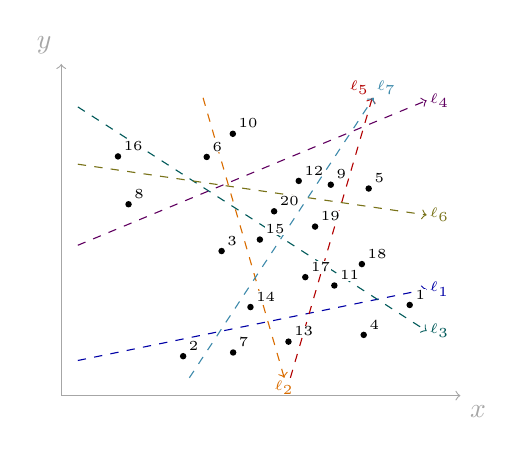
\begin{tikzpicture}[scale=0.78]
  \draw[->,gray!70] (0.45,0.45)--(6.95,0.45) node[below right] {$x$};
  \draw[->,gray!70] (0.45,0.45)--(0.45,5.85) node[above left] {$y$};
  \foreach \i/\linecolor/\xa/\ya/\xb/\yb/\labelanchor in {
    1/blue!65!black/0.72/1.022/6.4/2.182/west,
    2/orange!85!black/2.759/5.3/4.081/0.74/north,
    3/teal!70!black/0.72/5.151/6.4/1.502/west,
    4/violet!75!black/0.72/2.898/6.4/5.256/west,
    5/red!70!black/4.181/0.74/5.515/5.3/south east,
    6/olive!80!black/0.72/4.218/6.4/3.391/west,
    7/cyan!65!black/2.536/0.74/5.536/5.3/south west%
  } {
    \draw[->,color=\linecolor,dashed] (\xa,\ya)--(\xb,\yb);
    \node[anchor=\labelanchor,font=\tiny,text=\linecolor,inner sep=1pt]
      at (\xb,\yb) {$\ell_\i$};
  }
  \foreach \id/\x/\y in {
    1/6.124/1.926, 2/2.435/1.092, 3/3.061/2.804, 4/5.375/1.439,
    5/5.456/3.822, 6/2.819/4.336, 7/3.249/1.152, 8/1.546/3.566,
    9/4.839/3.884, 10/3.244/4.713, 11/4.897/2.243, 12/4.317/3.946,
    13/4.15/1.329, 14/3.531/1.892, 15/3.684/2.991, 16/1.374/4.345,
    17/4.424/2.379, 18/5.345/2.592, 19/4.583/3.202, 20/3.916/3.451
  } {
    \fill[black] (\x,\y) circle (1.5pt);
    \node[anchor=south west,font=\tiny,inner sep=0.4pt,fill=white,
          xshift=1.5pt,yshift=1.5pt] at (\x,\y) {\id};
  }
\end{tikzpicture}
\end{minipage}\hfill
\begin{minipage}[t]{0.60\textwidth}
\vspace{0pt}
\centering
{\small\textbf{One valid decision tree}\par}
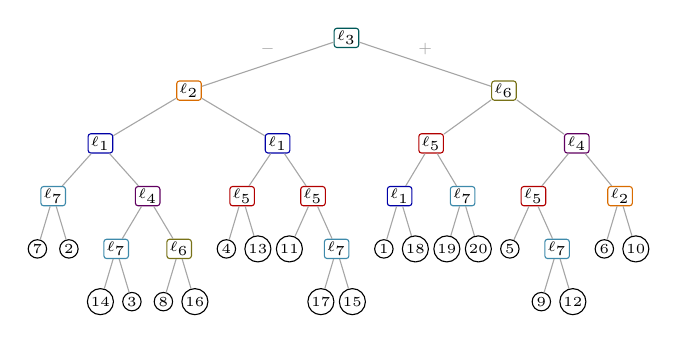
\begin{tikzpicture}[
  x=0.4cm,y=0.67cm,
  query/.style={rounded corners=1pt,fill=white,inner sep=1pt,font=\tiny},
  query1/.style={query,draw=blue!65!black},
  query2/.style={query,draw=orange!85!black},
  query3/.style={query,draw=teal!70!black},
  query4/.style={query,draw=violet!75!black},
  query5/.style={query,draw=red!70!black},
  query6/.style={query,draw=olive!80!black},
  query7/.style={query,draw=cyan!65!black},
  leaf/.style={draw,circle,fill=white,inner sep=0.7pt,font=\tiny},
  edge/.style={gray!70,thin}
]
  \node[query3] (n0) at (9.8125,0) {$\ell_3$};
  \node[query2] (n1) at (4.8125,-1) {$\ell_2$};
  \node[query1] (n2) at (2,-2) {$\ell_1$};
  \node[query7] (n3) at (0.5,-3) {$\ell_7$};
  \node[leaf] (n4) at (0,-4) {7};
  \node[leaf] (n5) at (1,-4) {2};
  \node[query4] (n6) at (3.5,-3) {$\ell_4$};
  \node[query7] (n7) at (2.5,-4) {$\ell_7$};
  \node[leaf] (n8) at (2,-5) {14};
  \node[leaf] (n9) at (3,-5) {3};
  \node[query6] (n10) at (4.5,-4) {$\ell_6$};
  \node[leaf] (n11) at (4,-5) {8};
  \node[leaf] (n12) at (5,-5) {16};
  \node[query1] (n13) at (7.625,-2) {$\ell_1$};
  \node[query5] (n14) at (6.5,-3) {$\ell_5$};
  \node[leaf] (n15) at (6,-4) {4};
  \node[leaf] (n16) at (7,-4) {13};
  \node[query5] (n17) at (8.75,-3) {$\ell_5$};
  \node[leaf] (n18) at (8,-4) {11};
  \node[query7] (n19) at (9.5,-4) {$\ell_7$};
  \node[leaf] (n20) at (9,-5) {17};
  \node[leaf] (n21) at (10,-5) {15};
  \node[query6] (n22) at (14.8125,-1) {$\ell_6$};
  \node[query5] (n23) at (12.5,-2) {$\ell_5$};
  \node[query1] (n24) at (11.5,-3) {$\ell_1$};
  \node[leaf] (n25) at (11,-4) {1};
  \node[leaf] (n26) at (12,-4) {18};
  \node[query7] (n27) at (13.5,-3) {$\ell_7$};
  \node[leaf] (n28) at (13,-4) {19};
  \node[leaf] (n29) at (14,-4) {20};
  \node[query4] (n30) at (17.125,-2) {$\ell_4$};
  \node[query5] (n31) at (15.75,-3) {$\ell_5$};
  \node[leaf] (n32) at (15,-4) {5};
  \node[query7] (n33) at (16.5,-4) {$\ell_7$};
  \node[leaf] (n34) at (16,-5) {9};
  \node[leaf] (n35) at (17,-5) {12};
  \node[query2] (n36) at (18.5,-3) {$\ell_2$};
  \node[leaf] (n37) at (18,-4) {6};
  \node[leaf] (n38) at (19,-4) {10};
  \foreach \parent/\child in {
    n3/n4, n3/n5, n7/n8, n7/n9, n10/n11, n10/n12,
    n6/n7, n6/n10, n2/n3, n2/n6, n14/n15, n14/n16,
    n19/n20, n19/n21, n17/n18, n17/n19, n13/n14, n13/n17,
    n1/n2, n1/n13, n24/n25, n24/n26, n27/n28, n27/n29,
    n23/n24, n23/n27, n33/n34, n33/n35, n31/n32, n31/n33,
    n36/n37, n36/n38, n30/n31, n30/n36, n22/n23, n22/n30%
  } {
    \draw[edge] (\parent)--(\child);
  }
  \draw[edge] (n0)--node[above,font=\tiny] {$-$} (n1);
  \draw[edge] (n0)--node[above,font=\tiny] {$+$} (n22);
\end{tikzpicture}
\end{minipage}
\caption{Seven randomly oriented supplied lines are drawn first, then
twenty hypotheses are placed in distinct cells of their arrangement.
The arrows orient the lines: the positive side is to the left of the
arrow. Each internal node queries the correspondingly colored line.
At every node the left branch is the negative answer and the right
branch is the positive answer. The leaf numbers match the point labels.
This valid tree has maximum depth five.}
\label{fig:problem-example}
\end{figure}

\subsection{Results and the main ideas}

We give polynomial-time constant-factor approximations for both
objectives:
\[
 4.464966
 \quad\text{for maximum depth},\qquad
 5.182976
 \quad\text{for expected depth}.
\]
The expected-depth bound applies to arbitrary strictly positive priors.
We first prove the individual-vertex factor below $5.445944$, then
improve it by applying the same polynomial coverage scheduler to
adjacent support blocks. Joint discovery and endpoint accounting
preserves the credit from a negative first endpoint. A coupled choice
of block orientations and geometric shift retains this saving through
the first two batches' coverage guarantees. Selectively querying both
endpoints after a positive answer also reveals pattern information;
a rational entropy lower bound credits it. Changing the initial
two coverage budgets and sometimes merging the first two geometric batches
gives the displayed expected-depth factor. A finite rational certificate
accounts for both delayed positive discoveries and the entire zero route.
For maximum depth, an exact rank-subset interval
scheduler with a logarithmic total cap, combined with the priority
fallback, lowers the polynomial factor from $5.464966$ to $4.464966$.
For every fixed $\varepsilon>0$, we give quasipolynomial-time
$(2+\varepsilon)$ approximations for both objectives, including
arbitrary-prior expected depth. A multigrade dynamic program schedules
adjacent hull-support blocks with nearly exact delay. Its direct
factors are below $4.464966$ for maximum depth and $3.7187$ for
expected depth; the former is also attained by the polynomial hybrid.
More significantly, the resulting bounds have leading
coefficient $2\lambda$ and an additive count or entropy potential.
Exact optimization of an initial $O(\log n)$ levels, followed by
these baseline trees, removes that potential from the final ratio.
The resulting running time is
$(mn)^{O(\varepsilon^{-1}\log n)}$ for $0<\varepsilon\le1$;
these guarantees are quasipolynomial.
Both exact threshold problems are strongly NP-complete. The
expected-depth reduction first uses strictly positive, polynomially
bounded integer weights before normalization. An exact geometric cloud
construction then gives strong NP-completeness under uniform priors.
The hardness instances
use integer-coordinate points on a parabola and only supplied line
queries. Constant-factor inapproximability remains open.

Two restricted algorithms sharpen this distinction. If a distinguished
hypothesis misses every designated cap and all caps have size at
most a fixed $b$, maximum depth is exactly solvable in polynomial
time. For weighted singleton/pair caps with all singleton tests and
a path-and-cycle pair graph, expected depth admits an EPTAS with
running time $2^{O(\varepsilon^{-3})}\operatorname{poly}(n,L)$.
The latter includes the weighted expected-depth hardness subclass:
an EPTAS is compatible with strong NP-completeness.
For uniform priors, a PTAS covers all fixed-size caps in convex
position with a distinguished all-miss hypothesis, even when singleton
tests are unavailable. Clearing short gaps separates bounded blocks;
an exact count-vector DP optimizes all interleavings of their queries.

The geometric structure behind the algorithms is easiest to see in a
state (the current set of hypotheses consistent with all answers so
far) where no line splits much of the remaining mass. Every test
then has a majority answer. The opposite, minority half-planes are
small, and Helly's theorem gives a point lying on all majority sides.
After translating this common witness to the origin, each query is
represented by a point in a normalized plane. The vertices of their
convex hull (the smallest convex set containing those points) suffice
to describe the relevant caps: each original cap is covered by at
most two adjacent vertex caps, and the vertex
answers of any one hypothesis form a \emph{circular interval}: a
consecutive block in the cyclic order in which the hull vertices
appear around the polygon, with wrap-around allowed. This turns the
geometric part of the problem into scheduling and searching over
circular intervals.

\paragraph{Maximum depth: schedule discovery against child heights.}
In a flat state, the algorithm first builds the recursive codes for
the hull-pattern classes. It then searches for a positive hull answer
using a schedule whose deadlines are derived from those codes' actual
heights. An optimal-tree path through the common witness supplies a
comparison schedule: classes that remain negative on a long prefix
have already saved that many queries when the optimal tree is
restricted to the class. Each original query has at most two
adjacent hull supports, so the comparison schedule consists of
singletons and adjacent pairs rather than arbitrary subsets.
Enumerating its first pair turns the remaining circular intervals
into ordinary intervals. A priority-greedy fallback preserves the
resulting credit simultaneously for every deadline. A second, exact
scheduler stores subsets of available ranks in a spatial Cartesian
tree. It is polynomial under a logarithmic total cap; simultaneous
recursive bounds for small and large optima make that cap sufficient
for the stronger general factor. Endpoint searches
are charged separately, with a smaller allowance when the discovery
path already supplies a negative neighbor. This is how the analysis
improves the constant without adding artificial height to a child
code.

\paragraph{Expected depth: pay once for learning a pattern.}
For expected depth, the algorithm again discovers the complete
hull-answer pattern before recursing. The analysis separates the
work into two parts. First, a class's constant prefix on an optimal
witness path disappears when the optimal tree is restricted to that
class; the saved queries pay for finding the class's first positive
hull answer. Second, the remaining endpoint information is paid for
by the entropy of the pattern that was not already revealed during
discovery. Exact weighted coverage at each integer budget, together
with a deterministic choice among shifted geometric batches, gives a
sharper first-cover bound. Adaptive block modes also credit the information
from a second endpoint answer, measured against a coarsened discovery
transcript whose cells retain the individual cap bound. A mass cap
on each adjacent support block
forces some targets into later blocks, where the discrete bound is
better; the waiting time of the all-zero pattern covers the
complementary case. Both the optimal-depth savings and the entropy
decrease telescope over the recursive partition, so no part of the
optimal cost is charged repeatedly.

\paragraph{Strong hardness: encode bin loads by matching choices.}
The reductions start from 3-Partition. Singleton and adjacent-pair
queries on disjoint odd paths make each item choose one of the
path's even-position vertices. A distinguished hypothesis forces
every optimal tree to make a maximum matching on these paths, so an
unmatched position represents a bin choice. For maximum depth,
clouds of points turn the resulting bin loads into counts of
branches with specified remaining heights. For expected depth,
carefully chosen weights turn them into a quadratic penalty for
unequal loads. The parabola construction realizes every query by an
explicit line. Replacing weight $w$ by a cloud of $w$ uniform points
with private singleton tests adds the same internal identification cost
to every matching invoice; this exact identity preserves the reduction.

Section~\ref{sec:preliminaries} fixes notation and provides the
coding, information, and geometry preliminaries.
Sections~\ref{sec:geometry} and~\ref{sec:worst} develop the
common-witness geometry and the maximum-depth algorithm.
Section~\ref{sec:mass-improvement}
establishes the initial expected-depth guarantee, and
Section~\ref{sec:polynomial-blocks} improves its polynomial factor.
Section~\ref{sec:adaptive-blocks} gives the sharper adaptive-mode
expected-depth algorithm, Section~\ref{sec:first-phase}
improves its initial batches, and Section~\ref{sec:polynomial-slots}
gives the polynomial maximum-depth improvement.
Section~\ref{sec:boundaries}
shows how to handle hypotheses on query lines, and
Section~\ref{sec:hardness} gives the reductions.
Section~\ref{sec:uniform-hardness} transfers hardness to uniform priors
through an exact geometric cloud identity. We first establish
the common-witness geometry and the accounting inequalities shared
by the algorithms; the later sections then apply them to the two
objectives separately. Section~\ref{sec:quasipolynomial} gives the
quasipolynomial improvements for both objectives using a spatial
multigrade dynamic program.
Section~\ref{sec:small-caps} gives the stronger small-cap algorithms.

\section{Preliminaries and basic accounting}
\label{sec:preliminaries}

We collect the model, coding and information inequalities, and
geometric terminology used by the algorithms. Reduction-specific
graph and complexity definitions are given in
Section~\ref{sec:hardness}.
For a positive integer $r$, write $[r]=\{1,\ldots,r\}$.
The notation $|S|$ denotes set cardinality, while $|Q|$ denotes
the length of a word, vector, or sequence when $Q$ is such an object.
The indicator $\mathbf1[P]$ is one if statement $P$ holds and zero
otherwise. We also write $\mathbf1_A(x)=\mathbf1[x\in A]$ for
the indicator function of a set $A$.
The floor $\lfloor x\rfloor$ and ceiling $\lceil x\rceil$
are the greatest integer at most $x$ and the least integer at least
$x$, respectively. For planar vectors,
$x\cdot y=x_1y_1+x_2y_2$ is the dot product.

\subsection{Line-query model and objectives}

Let $\HH\subset\mathbb R^2$ be $n\ge2$ distinct points. A finite family
$\LL$ of $m$ supplied lines separates every pair of hypotheses,
meaning that every two distinct points receive different answers to
at least one line. Write a line as the zero set of an affine function
$f_\ell(x)=a_\ell\cdot x+b_\ell$, where
$a_\ell\in\mathbb R^2\setminus\{0\}$ and $b_\ell\in\mathbb R$.
Querying $\ell$ returns the sign of $f_\ell(h)$ for
the hidden point $h$. Every query contributes one to the depth.
Unless explicitly stated otherwise, no hypothesis lies on a supplied
line, so the answer is binary.
Section~\ref{sec:boundaries} treats a third, on-line outcome.

After any sequence of queries and answers, the current \emph{state}
is the set of hypotheses whose signs on all queried lines agree with
the answers received. For a state $S$ and a supplied line $\ell$,
write
\[
 S_\ell^-=\{h\in S:f_\ell(h)<0\},\qquad
 S_\ell^+=\{h\in S:f_\ell(h)>0\}.
\]
These are the two answer classes; the line \emph{splits} $S$ when
both classes are nonempty.

\begin{definition}[Line-query decision trees]\label{def:decision-tree}
A binary line-query decision tree is a finite rooted tree whose
internal nodes are labeled by supplied lines and whose two outgoing
edges are labeled by their negative and positive answers. A
hypothesis follows the edge matching its answer at each query.
An \emph{identifying} tree for $S$ has hypothesis labels at its leaves
and sends every $h\in S$ to a leaf labeled $h$. The root has depth
zero; a leaf's depth is the number of queries on its root-to-leaf path,
and the tree's \emph{height} is its largest leaf depth.

A \emph{partial decision tree}, or \emph{stage}, may instead stop at
leaves labeled by nonempty subsets of $S$. Each leaf is labeled by
exactly the hypotheses compatible with its path, so these output
classes partition $S$. Attaching an identifying tree for each class
produces a complete identifying tree.
\end{definition}

We suppress a query
whenever its answer is already determined by the current candidate
set. In particular, a line is never queried twice on one path.
The resulting tree is \emph{proper}: both children of every internal
node contain hypotheses. A proper binary tree on $n$ hypotheses
has $n-1$ internal nodes and depth at most $n-1$: if $I$ is its
number of internal nodes, counting edges gives $2I=I+n-1$, so
$I=n-1$ and every path has at most that many queries. This convention
does not restrict the optimum: a query with only one nonempty
outcome can be deleted, and repeated queries have already known
answers.

A \emph{transcript} records the queries and answers observed along
a path. In a fixed binary tree the previous answers determine the
next query, so the transcript can also be represented by its answer
word, encoding negative as $0$ and positive as $1$.
A \emph{cached answer} is an answer already learned on that path;
reusing it or inferring a constant answer costs no additional query.
For nonempty $A\subseteq S$, the \emph{restriction} $T|_A$ is obtained
by deleting leaves outside $A$, deleting empty branches, and
contracting queries with only one surviving outcome. It is a valid
tree on $A$, and no surviving hypothesis's depth increases.

\begin{definition}[Membership answers and spines]\label{def:membership-spine}
A \emph{membership interpretation} designates one answer class $A$
of a supplied binary query. Its answer is a \emph{hit} when $h\in A$
and a \emph{miss} otherwise. A hit may be either affine sign;
interpreting the answer changes neither the supplied line nor its cost.

The \emph{spine} of a distinguished hypothesis is its root-to-leaf
path. Another hypothesis \emph{exits} that path at its first
different answer; the attached subtree is its local exit code.
If this occurs at query position $j$, a local depth $d$ contributes
total depth $j+d$.
If every designated membership set excludes the distinguished
hypothesis, its spine is an all-miss route and exits occur at first hits.
A point $p$ on no supplied line similarly determines a
\emph{witness path}, even when $p\notin\HH$.
\end{definition}

Let $d_T(h)$ be the number of queries on the path followed by $h$,
stopping at its output leaf; for an identifying tree that leaf names $h$.
For a tree $T$ identifying a candidate set $S\subseteq\HH$, define
\[
 c_{\mathrm W}(T)=\max_{h\in S}d_T(h).
\]
For expected depth, let $\pi_h>0$ with $\sum_h\pi_h=1$, write
$w(S)=\sum_{h\in S}\pi_h$, and define
\[
 c_{\mathrm E}(T)=\sum_{h\in S}\pi_h d_T(h).
\]
The weights in $c_{\mathrm E}(T)$ are the original probabilities;
they are not renormalized when a tree identifies a restricted state.
Thus $c_{\mathrm E}(T)/w(S)$ is the conditional expected cost,
whereas $c_{\mathrm E}(T)$ is that state's contribution to the
original expectation. At the root, where $w(\HH)=1$, the two agree.
Define the corresponding optima by
\[
 \OPT_{\mathrm W}(S)=\min_{T\text{ identifying }S}c_{\mathrm W}(T),
 \qquad
 \OPT_{\mathrm E}(S)=\min_{T\text{ identifying }S}c_{\mathrm E}(T).
\]
We set both optima to zero on the empty set and on singletons.
Hypothesis weights used later in the hardness proof specify these
probabilities; they do not alter how queries are counted. Keeping
weights unnormalized means that the expected costs of disjoint
recursive states add directly.

More explicitly, if positive raw weights $\omega_h$ are supplied,
put $\Omega=\sum_{h\in\HH}\omega_h$ and $\pi_h=\omega_h/\Omega$.
Then, also on a restricted state,
\[
 \sum_{h\in S}\omega_h d_T(h)=\Omega c_{\mathrm E}(T).
\]
Thus normalizing weights divides both a weighted cost and its
decision threshold by the same $\Omega$, without changing which
tree is optimal. Raw weights are not costs of individual queries:
every query still costs one.

If $S_\ell^-$ and $S_\ell^+$ are the two answer classes in $S$,
the optimality recurrences on nonsingleton states are
\[
 \begin{split}
 \OPT_{\mathrm W}(S)&=1+\min_{\ell\text{ splitting }S}
                    \max\{\OPT_{\mathrm W}(S_\ell^-),
                         \OPT_{\mathrm W}(S_\ell^+)\},\\
 \OPT_{\mathrm E}(S)&=w(S)+\min_{\ell\text{ splitting }S}
                    \{\OPT_{\mathrm E}(S_\ell^-)
                      +\OPT_{\mathrm E}(S_\ell^+)\}.
 \end{split}
\]
Algorithm~\ref{alg:exact-tree} implements these recurrences on the
small local states used later. These recurrences define the quantities used in the analysis; the
approximation algorithms do not evaluate them. The first recurrence
charges one query on every path and then takes the harder child. In
the second, that query contributes the total state mass $w(S)$, and
the two child contributions add because their hypothesis sets are
disjoint.

\begin{algorithm}[H]
\caption{Exact supplied-query Bellman recursion (small local states)}
\label{alg:exact-tree}
\KwIn{State $S$; objective $o\in\{\mathrm W,\mathrm E\}$; original weights $\pi_h$.}
\KwOut{An optimal supplied-query tree and its cost.}
\If{$|S|\le1$}{\KwRet the leaf of cost zero\;}
\If{the memoized value for $(S,o)$ exists}{\KwRet that value and tree\;}
\ForEach{supplied line $\ell$ splitting $S$}{
  $(T_-,v_-)\gets\ExactTree(S_\ell^-,o)$;
  $(T_+,v_+)\gets\ExactTree(S_\ell^+,o)$\;
  $v_\ell\gets1+\max\{v_-,v_+\}$ if $o=\mathrm W$,
  and $v_\ell\gets w(S)+v_-+v_+$ otherwise\;
}
Memoize the minimum $v_\ell$ and the tree joining its stored children\;
\KwRet the memoized cost and tree\;
\end{algorithm}

Algorithm~\ref{alg:exact-tree} takes $2^{O(|S|)}\operatorname{poly}(m,L)$
time with bit-mask states. It is used only on bounded local sets;
the general approximation algorithms never call it on the full input.


All logarithms are natural unless a base is displayed, and
we use $0\ln0=0$, the continuous extension at zero.
Coordinates, line coefficients, and probabilities are rational
and explicitly given by binary-encoded numerators and denominators.
Polynomial time means polynomial in this input's bit length,
not in the magnitudes of its numerical values.
The \emph{decision version} of either objective asks, given an
instance and a threshold $K$, whether a legal identifying tree
has cost at most $K$. For maximum depth the threshold can be
an integer; for expected depth it is rational and the prior is
part of the input.
An \emph{$\alpha$-approximation} for a minimization objective returns
a feasible tree whose cost is at most $\alpha$ times the optimum
on every valid input. A deterministic guarantee concerns the one
tree returned, not an average over randomly chosen trees.
Whenever an algorithm permits several choices, fix a deterministic
tie-breaking rule, such as the input order.

\begin{symboltable}
$\HH,\LL;\ n,m$ & Hypothesis points, supplied lines, and their counts.\\
$S,\ S_\ell^-,S_\ell^+$ & Current state and its negative and positive answer classes for line $\ell$.\\
$d_T(h)$ & Number of queries on the path for hypothesis $h$ in tree $T$.\\
$c_{\mathrm W}(T),\ \OPT_{\mathrm W}(S)$ & Maximum path depth and its minimum over identifying trees for $S$.\\
$\pi_h,\ w(S)$ & Root prior probability of $h$ and the original probability mass of state $S$.\\
$c_{\mathrm E}(T),\ \OPT_{\mathrm E}(S)$ & Expected depth using the original probabilities and its minimum over identifying trees for $S$.\\
$\mathcal E(S)$ & State-mass-weighted entropy of the conditional distribution on $S$.\\
$\Pi,\ \Delta_{\mathrm E}(S,\Pi),\ I(S,\Pi)$ & A partition of $S$, the decrease in optimal expected depth, and the information gained from its class label.\\
$\omega_h,\ \Omega$ & Optional raw positive weights and their total; $\pi_h=\omega_h/\Omega$.\\
\end{symboltable}

\begin{definition}[Balanced and flat states]\label{def:balanced}
Fix $0<\delta<1/3$. A nonsingleton state $S$ is
\emph{count-balanced} if some supplied line has at least
$\delta|S|$ hypotheses on each side. Otherwise it is
\emph{count-flat}. In the flat case, every line has a unique
\emph{majority answer}, on the side containing more than half of $S$.
We call this its \emph{frozen answer} and write $C_\ell$ for the
open half-plane on the opposite side. Its induced answer class
$C_\ell\cap S$ is the \emph{minority cap}, of size less than
$\delta|S|$. We also use ``cap'' for the corresponding half-plane
when discussing its geometry.
\end{definition}

The expected-depth algorithm uses probability mass in place of
cardinality: $S$ is \emph{mass-balanced} if some line has
$w(S_\ell^-),w(S_\ell^+)\ge\delta w(S)$, and \emph{mass-flat}
otherwise. In a mass-flat state, freezing the mass-majority answer
gives $w(C_\ell\cap S)<\delta w(S)$.

Throughout the pseudocode, tables contain only realized hypotheses or
patterns, ties use input order, and a returned tree is contracted whenever
a query has a constant answer. Cached answers, the origin marker, and
infeasible branches therefore create no additional supplied query. The
numerical parameters and their certificates are stated with the analysis
of each routine.



\begin{figure}[htbp]
\centering
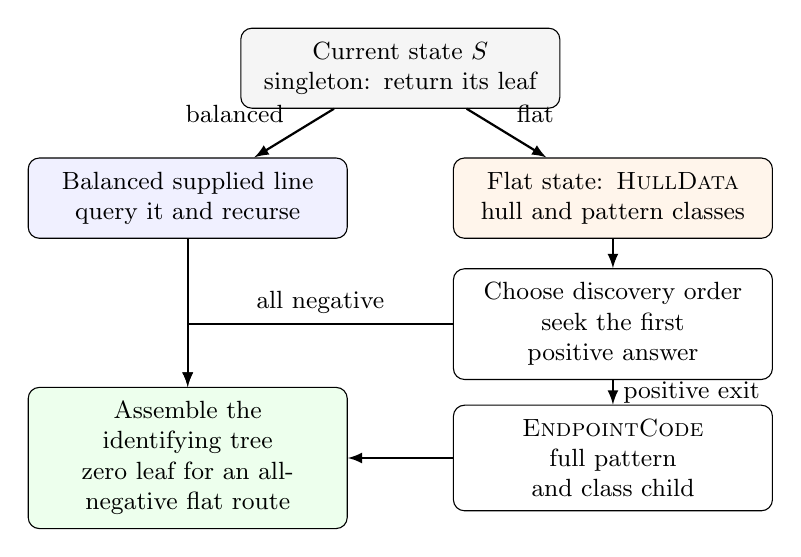
\begin{tikzpicture}[every node/.style={font=\small},
  box/.style={draw,rounded corners,align=center,inner sep=5pt,text width=3.7cm},
  arr/.style={-latex,thick}]
  \node[box,fill=gray!8] (state) at (0,0) {Current state $S$\\singleton: return its leaf};
  \node[box,fill=blue!6] (balanced) at (-2.7,-1.65)
    {Balanced supplied line\\query it and recurse};
  \node[box,fill=orange!8] (flat) at (2.7,-1.65)
    {Flat state: \HullData\\hull and pattern classes};
  \node[box] (discover) at (2.7,-3.25)
    {Choose discovery order\\seek the first positive answer};
  \node[box] (decode) at (2.7,-4.95)
    {\EndpointCode\\full pattern and class child};
  \node[box,fill=green!7] (output) at (-2.7,-4.95)
    {Assemble the identifying tree\\zero leaf for an all-negative flat route};
  \draw[arr] (state) -- node[above left]{balanced} (balanced);
  \draw[arr] (state) -- node[above right]{flat} (flat);
  \draw[arr] (flat) -- (discover);
  \draw[arr] (discover) -- node[right]{positive exit} (decode);
  \draw[arr] (discover.west) -- node[above]{all negative} (-2.7,-3.25)
    -- (output.north);
  \draw[arr] (decode) -- (output);
  \draw[arr] (balanced) -- (output);
\end{tikzpicture}
\caption{The common recursive structure. Arrows describe the output of
one stage passed to the next. The maximum-depth routines construct class
children before choosing the schedule, so their stored heights can set
deadlines; expected-depth routines use original prior masses. The flat
stage has an all-negative leaf only when the zero pattern is present.
Scheduling and decoding use supplied hull lines.}
\label{fig:recursive-procedure-flow}
\end{figure}



\subsection{Binary codes and ordered comparisons}

\begin{definition}[Binary codes and prefix codes]\label{def:binary-code}
A \emph{binary word} is a finite sequence of bits from $\{0,1\}$;
$\{0,1\}^*$ includes the empty word $\varepsilon$, of length zero.
A \emph{binary code} on a finite nonempty alphabet $\mathcal A$ is
an injective map $c:\mathcal A\to\{0,1\}^*$. The word $c(a)$ is
the \emph{codeword} for $a$, and $\ell_a=|c(a)|$ is its length.
A word $u$ is a \emph{prefix} of $v$ if $v$ starts with all the
bits of $u$. A code is \emph{prefix-free}, or a \emph{prefix code},
if no codeword is a prefix of another distinct codeword.
\end{definition}

For a distribution $(q_a)$ on the alphabet, the code's maximum
length is $\max_a\ell_a$ and its expected length is
$\sum_a q_a\ell_a$.
The prefix tree of a code has one node for each prefix of a
codeword, with the empty prefix at the root and edges appending
$0$ or $1$. For a prefix code its codewords are exactly the leaves,
at depths $\ell_a$. Conversely, the root-to-leaf answer words of
any binary decision tree form a prefix code. Unary nodes, which
have only one child, can be contracted without increasing any depth.
The empty word is permissible only when the alphabet is a singleton.
For example, $c(a)=0$, $c(b)=10$, and $c(c)=11$ form a prefix code
with lengths $1,2,2$.

\begin{definition}[Alphabetic codes]\label{def:alphabetic-code}
For an ordered alphabet $y_1<\cdots<y_r$, a prefix code is
\emph{alphabetic} if its codewords occur in that same lexicographic
order, with $0<1$. An \emph{ordered threshold comparison} asks
whether the unknown outcome is at most $y_j$ for some $j$.
\end{definition}

In an alphabetic prefix tree, the outcomes below each node form
a consecutive range. After unary nodes are contracted, its two
children separate that range at one threshold. Thus an alphabetic
code can be implemented by ordered threshold comparisons whenever
those comparisons are available. The code bits label the two
ordered ranges; a line's raw sign answer is routed to the matching
range, even if its sign encoding uses the opposite bit. This
relabeling adds no query. An arbitrary prefix code need
not be executable by the supplied line family. When we call an
identifying decision tree a \emph{code}, its internal queries must
still be supplied lines. Section~\ref{sec:endpoint-geometry} verifies
that the comparisons used for its endpoint codes are available.

A word $b_1\cdots b_\ell$ specifies the half-open \emph{dyadic cell}
\[
 D(b_1\cdots b_\ell)=
 \left[\sum_{j=1}^{\ell}b_j2^{-j},
       \sum_{j=1}^{\ell}b_j2^{-j}+2^{-\ell}\right)
 \subseteq[0,1).
\]
The empty word specifies $[0,1)$. Such cells are nested or disjoint;
one word is a prefix of another exactly when its cell contains
the other's cell. Half-open endpoints avoid ambiguity at dyadic
rationals.

\begin{theorem}[Kraft's inequality for binary prefix codes]
\label{thm:kraft}
Every finite binary prefix code has lengths satisfying
\[
 \sum_{a\in\mathcal A}2^{-\ell_a}\le1.
\]
Conversely, nonnegative integer lengths $(\ell_a)_{a\in\mathcal A}$
are realizable by a binary prefix code if this inequality holds.
The converse does not prescribe alphabetic order or guarantee
implementation by a restricted query family.
\end{theorem}
\begin{proof}
For necessity, prefix-free codewords specify disjoint dyadic cells
inside $[0,1)$, whose widths are $2^{-\ell_a}$.

For sufficiency, reorder the lengths as
$\ell_1\le\cdots\le\ell_r$ and put
$s_i=\sum_{j<i}2^{-\ell_j}$. Each $s_i$ is an integer multiple
of $2^{-\ell_i}$ because every earlier length is at most $\ell_i$.
The intervals $[s_i,s_i+2^{-\ell_i})$ are therefore dyadic cells
of the prescribed depths. They are disjoint and lie in $[0,1)$
by the assumed bound. Their binary descriptions give the required
prefix code; assign them back to the original symbols.
\end{proof}

The code $0,10,11$ has Kraft sum
$2^{-1}+2^{-2}+2^{-2}=1$. More generally, equality holds for a
proper binary tree because its two child cells partition each
internal node's cell. The coding facts here and the information
inequalities below are standard; see Cover and Thomas~\cite{ct2006}.

\subsection{Entropy and information inequalities}

\begin{definition}[Entropy and conditional entropy]\label{def:entropy}
A \emph{probability vector} $(q_i)$ has nonnegative entries summing
to one; its \emph{support} consists of the indices with $q_i>0$.
For a finite random variable $Y$ with probabilities
$q_y=\Pr[Y=y]$, its Shannon entropy in natural-log units is
\[
 H(Y)=-\sum_y q_y\ln q_y.
\]
We also write $H(q)$ for the entropy of a probability vector.
The joint entropy $H(Y,Z)$ is the entropy of the pair $(Y,Z)$.
For $Z$ with finite support, conditional entropy is
\[
 H(Y\mid Z)=
 \sum_{z:\Pr[Z=z]>0}\Pr[Z=z]\,H(Y\mid Z=z),
\]
where the inner entropy uses
$\Pr[Y=y\mid Z=z]=\Pr[Y=y,Z=z]/\Pr[Z=z]$.
Conditioning on several variables means
conditioning on their tuple. Entropy in bits is $H(Y)/\ln2$.
For a function $g$ of a finite random variable,
$\mathbb E[g(Y)]=\sum_y q_y g(y)$.
The \emph{binary entropy} is
$h(t)=-t\ln t-(1-t)\ln(1-t)$ for $0\le t\le1$.
\end{definition}

For nonempty $S$, the conditional hypothesis probabilities are
$q_h=\pi_h/w(S)$. Define the \emph{weighted state entropy} by
\[
 \mathcal E(S)=w(S)H(q)
       =\sum_{h\in S}\pi_h\ln\frac{w(S)}{\pi_h},
 \qquad \mathcal E(\varnothing)=0.
\]
It is zero on singletons. Like $c_{\mathrm E}$, this quantity
includes the original state mass rather than renormalizing it away.

\begin{lemma}[Log-sum inequality]\label{lem:log-sum}
For nonnegative $a_i$ and positive $b_i$, with
$A=\sum_i a_i>0$ and $B=\sum_i b_i$, one has
\[
 \sum_i a_i\ln\frac{a_i}{b_i}\ge A\ln\frac AB,
\]
with zero summands interpreted by continuity.
\end{lemma}
\begin{proof}
Put $q_i=a_i/A$ and $r_i=b_i/B$.
The inequality $-\ln x\ge1-x$ for $x>0$ follows because
$x-1-\ln x$ has its minimum zero at $x=1$. Hence
\[
 \sum_{i:q_i>0}q_i\ln\frac{q_i}{r_i}
 \ge\sum_{i:q_i>0}(q_i-r_i)
 =1-\sum_{i:q_i>0}r_i\ge0.
\]
Multiplying by $A$ and adding $A\ln(A/B)$ proves the assertion.
\end{proof}

\begin{lemma}[Entropy chain rule]\label{lem:entropy-chain-rule}
For finite random variables,
\[
 H(Y,Z)=H(Z)+H(Y\mid Z),\qquad
 H(Y,Z\mid W)=H(Y\mid W)+H(Z\mid Y,W).
\]
If $Z$ is determined by $Y$, then
$H(Y)=H(Z)+H(Y\mid Z)$. Also,
$0\le H(Y)\le\ln|\operatorname{supp}(Y)|$ and
$H(Y\mid Z)\ge0$; in particular $0\le h(t)\le\ln2$.
\end{lemma}
\begin{proof}
Substitute
$\Pr[Y=y,Z=z]=\Pr[Z=z]\Pr[Y=y\mid Z=z]$ into the joint
entropy sum. Taking its logarithm separates the two terms of the
first identity. Apply the same identity under each value of $W$
and average to obtain the conditional form. If $Z$ is determined
by $Y$, the pair $(Y,Z)$ has the same entropy as $Y$.
Entropy and conditional entropy are nonnegative because their
summands are $-q\ln q\ge0$ for $q\in[0,1]$.
Applying Lemma~\ref{lem:log-sum} to $Y$'s distribution and the
uniform distribution on its support gives the upper bound.
\end{proof}

\begin{lemma}[Alphabetic threshold codes]\label{lem:alphabetic-endpoints}
Let $Y$ have finite ordered support, and let $H(Y)$ be its entropy
with natural logarithms. There is an explicit alphabetic threshold
code with depth on outcome $y$ at most
$\log_2(1/\Pr[Y=y])+2$.
In particular its expected depth is at most
\[
 \frac{H(Y)}{\ln2}+2.
\]
This is a dyadic prefix-code construction; see Cover and
Thomas~\cite{ct2006} for the general coding background. The short
proof here also verifies the extra alphabetic (order-preserving)
property needed for threshold queries.
An optimal expected-depth threshold tree can also be computed by
a polynomial interval dynamic program. The explicit code is used
when the pointwise depth bound is needed.
\end{lemma}
\begin{proof}
For an ordered outcome $y$ of probability $a$, let
$F_y=\sum_{y'<y}\Pr[Y=y']$. Its \emph{cumulative-probability
interval} is $[F_y,F_y+a)$, with midpoint $m_y=F_y+a/2$.
The \emph{midpoint-dyadic code} chooses the dyadic cell containing
$m_y$ at depth $\ell_y=\lceil\log_2(2/a)\rceil$, in the sense
of the cells defined before Theorem~\ref{thm:kraft}.
The cell's width is at most $a/2$, so the entire cell lies in
the outcome's interval. These cells are disjoint and appear in
outcome order. Their binary descriptions form a prefix-free
alphabetic code. Since $\lceil x\rceil\le x+1$, their lengths
satisfy
\[
 \left\lceil\log_2\frac2a\right\rceil
 \le\log_2\frac1a+2.
\]
After unary nodes are contracted, each internal node separates
two consecutive outcome ranges and is a threshold comparison.
Taking expectation of this pointwise bound gives
\[
 \sum_y\Pr[Y=y]\left(\log_2\frac1{\Pr[Y=y]}+2\right)
 =\frac{H(Y)}{\ln2}+2.
\]

To minimize expected depth, let $D_{i,j}$ be the minimum weighted
depth contributed by outcomes $y_i,\ldots,y_j$, using their original
probabilities $p_a=\Pr[Y=y_a]$. Set $D_{i,i}=0$. For $i<j$, a root
threshold after $y_t$ contributes $\sum_{a=i}^j p_a$, so
\[
 D_{i,j}=\sum_{a=i}^j p_a+
       \min_{i\le t<j}\{D_{i,t}+D_{t+1,j}\}.
\]
This interval dynamic program uses $O(r^3)$ rational arithmetic
operations. The resulting optimal alphabetic tree satisfies the
expected-depth bound; no long binary expansion of a very small
probability is required. It need not preserve the pointwise bound,
which uses the explicit midpoint-dyadic construction.
\end{proof}

\begin{algorithm}[H]
\caption{Alphabetic code on ordered outcomes}
\label{alg:alphabetic-code}
\KwIn{Ordered outcomes $y_1<\cdots<y_r$ of positive rational masses $a_i$;
mode \emph{pointwise} or \emph{expected}.}
\KwOut{A threshold-comparison tree.}
\If{$r=1$}{\KwRet its zero-depth leaf\;}
\eIf{mode is \emph{pointwise}}{
  Normalize $q_i=a_i/\sum_j a_j$ and put $F_i=\sum_{j<i}q_j$\;
  \ForEach{$i$}{
    Find $d_i=\lceil\log_2(1/q_i)\rceil+1$ by rational powers-of-two comparisons\;
    Take the depth-$d_i$ dyadic cell containing $F_i+q_i/2$ as codeword $i$\;
  }
  Build the alphabetic prefix tree and contract unary nodes\;
}{
  Set $D_{i,i}=0$\;
  \For{$h=2,\ldots,r$}{
    \ForEach{$[i,j]$ of length $h$}{
      $D_{i,j}\gets\sum_{a=i}^j a_a+min_{i\le t<j}(D_{i,t}+D_{t+1,j})$\;
      Store a minimizing split after $y_t$\;
    }
  }
  Reconstruct the stored interval splits\;
}
\KwRet the ordered tree, implementing each split by its available threshold\;
\end{algorithm}

The pointwise mode preserves the per-outcome bound; the expected mode
has $O(r^3)$ arithmetic complexity and avoids long expansions for small
priors. Their distinct roles are proved in
Lemma~\ref{lem:alphabetic-endpoints}.


\subsection{Restriction and recursive accounting}

Two lower bounds will account for different kinds of work.
Restriction measures which queries are unnecessary once a class
is known. Entropy measures the information learned from a class label.

\begin{definition}[Partitions and refinement]\label{def:partitions}
A \emph{partition} $\Pi$ of $S$ is a family of pairwise disjoint
nonempty subsets whose union is $S$. We say $\Pi$ \emph{refines}
$\mathcal R$, or $\mathcal R$ is \emph{coarser} than $\Pi$, if
every class of $\Pi$ is contained in a class of $\mathcal R$.
The output classes of a partial decision tree form a partition.
\end{definition}

\begin{lemma}\label{lem:restriction}
For pairwise disjoint subsets $S_1,\ldots,S_k$ of a state $S$,
\[
 \sum_i \OPT_{\mathrm E}(S_i)\le \OPT_{\mathrm E}(S),\qquad
 \OPT_{\mathrm W}(S_i)\le \OPT_{\mathrm W}(S).
\]
Moreover,
\[
 \OPT_{\mathrm E}(S)\ge\frac{\mathcal E(S)}{\ln2},
 \qquad
 \OPT_{\mathrm W}(S)\ge\frac{\ln|S|}{\ln2}
 \quad\text{for nonempty }S.
\]
\end{lemma}
\begin{proof}
Restrict an optimal tree on $S$ to each $S_i$ and contract its constant
queries. No hypothesis's depth increases. Summing over disjoint
subsets proves the expected-depth inequality; restricting a
maximum-depth-optimal tree proves the second inequality.

For entropy, assume $S\ne\varnothing$; the empty-state case is
immediate. Let $q_h=\pi_h/w(S)$. The leaf transcripts are a binary
prefix code as in Definition~\ref{def:binary-code}: a transcript
cannot continue beyond a leaf. Theorem~\ref{thm:kraft} therefore
gives $\sum_h2^{-\ell_h}\le1$ for their lengths.
Apply Lemma~\ref{lem:log-sum}, dividing by $\ln2$ to use base two, with
$\ell_h=d_T(h)$ and $q_h=\pi_h/w(S)$:
\[
 \begin{aligned}
 \sum_h q_h\ell_h-\sum_hq_h\log_2\frac1{q_h}
 &=\sum_hq_h\log_2\frac{q_h}{2^{-\ell_h}}\\
 &\ge \log_2\frac{\sum_hq_h}{\sum_h2^{-\ell_h}}
 \ge0.
 \end{aligned}
\]
The first inequality is the log-sum inequality, and the second uses
$\sum_hq_h=1$ and Kraft's bound. Hence every tree identifying $S$
satisfies
\[
 c_{\mathrm E}(T)=w(S)\sum_hq_hd_T(h)
 \ge w(S)\sum_hq_h\log_2\frac1{q_h}
 =\frac{w(S)}{\ln2}\sum_hq_h\ln\frac1{q_h}
 =\frac{\mathcal E(S)}{\ln2}.
\]
Minimizing gives the expected-depth lower bound.
For the maximum-depth bound, prove by induction on $d$ that a binary
tree of height $d$ has at most $2^d$ leaves. The claim is immediate
for $d=0$; for $d>0$, the root has at most two child subtrees, each
of height at most $d-1$, so together they have at most
$2\cdot2^{d-1}=2^d$ leaves. Thus $|S|\le2^d$, or
$d\ge\log_2|S|=\ln|S|/\ln2$.
\end{proof}

We call a state quantity used to account for progress a
\emph{potential}. For expected depth, the relevant potentials
are $\OPT_{\mathrm E}$ and $\mathcal E$; their decrements are the
parent value minus the sum of the child values.
For a nonempty state $S$ and a partition $\Pi$ of it, write
\[
 \begin{split}
  \Delta_{\mathrm E}(S,\Pi)&=\OPT_{\mathrm E}(S)
                     -\sum_{A\in\Pi}\OPT_{\mathrm E}(A),\\
  I(S,\Pi)&=\mathcal E(S)-\sum_{A\in\Pi}\mathcal E(A)
           =\sum_{A\in\Pi}w(A)\ln\frac{w(S)}{w(A)}.
  \end{split}
 \]
  Let $X$ be a random hypothesis with
 $\Pr[X=h]=\pi_h/w(S)$, and let $P$ be its class label under $\Pi$.
 Then
 \[
  I(S,\Pi)=w(S)H(P),\qquad
  H(P)=-\sum_{A\in\Pi}\frac{w(A)}{w(S)}
                          \ln\frac{w(A)}{w(S)}.
 \]
 Thus $I(S,\Pi)$ is the state mass times the Shannon entropy of the
 class label, measured in natural-log units. This is the partition
 form of the chain rule in Lemma~\ref{lem:entropy-chain-rule}.
 Both quantities are nonnegative. The first is the decrease in
optimal expected depth when the class is revealed; the second is
the weighted entropy of that class. Their differences telescope
over any recursive partition ending in singletons. More explicitly,
if each internal state $S$ is split into classes $\Pi_S$, then
\[
 \sum_{S\ {\rm internal}}\Delta_{\mathrm E}(S,\Pi_S)
       =\OPT_{\mathrm E}(\HH),\qquad
 \sum_{S\ {\rm internal}}I(S,\Pi_S)=\mathcal E(\HH).
\]
Every child term cancels against that child's term at its own split,
and the terminal singleton potentials are zero. The approximation
proofs will bound each stage by these local decreases; this
cancellation is what prevents repeated charges to the same optimum.

\subsection{Convex geometry and finite set systems}

\begin{definition}[Planar convexity]\label{def:convex-geometry}
A set is \emph{convex} if it contains the segment joining any two
of its points. A \emph{convex combination} is a sum
$\sum_j\lambda_j u_j$ with $\lambda_j\ge0$ and
$\sum_j\lambda_j=1$. The \emph{convex hull}
$\operatorname{conv}(U)$ of a finite nonempty point set $U$ is the set of
its convex combinations. A \emph{vertex}, or extreme point, cannot
be expressed as a convex combination of other points of the hull.
The hull is the convex hull of its vertices; set
$\operatorname{conv}(\varnothing)=\varnothing$ by convention.

A nonempty planar hull has affine dimension zero, one, or two according
as it is a point, a nontrivial segment, or has nonempty planar
interior. In dimension two it is a convex polygon, whose vertices
have a cyclic boundary order; its \emph{edges} join consecutive
vertices. A \emph{supporting line} meets a convex set and leaves
it entirely on one closed side. It \emph{exposes} a point if that
point is its unique intersection with the set. A finite point
set is in \emph{strictly convex position} if every point is a
vertex of its hull.
\end{definition}

An open half-plane has the form $\{x:a\cdot x>b\}$ for $a\ne0$;
replacing $>$ by $\ge$ gives its closed counterpart. A point is
\emph{strictly} on a chosen side when it is in that open half-plane,
not on its boundary. A common strict \emph{witness} for several
chosen sides is a point in all their open half-planes; it need
not itself be a hypothesis.

\begin{theorem}[Planar Helly theorem]\label{thm:helly}
If every subfamily of at most three
sets in a finite family of planar convex sets has nonempty
intersection, then the whole family has nonempty intersection.
The sets may be open.
\end{theorem}
This is the standard planar form; see Matou\v{s}ek~\cite{matousek2002}.

\begin{definition}[Covers and hitting sets]\label{def:covers-and-hitting}
A finite \emph{set system} consists of a universe $U$, a candidate
set $V$, and supplied subsets $F_v\subseteq U$ indexed by $v\in V$.
A \emph{cover} of $U$ is a choice of these sets whose union contains
every element of $U$.
In the equivalent demand formulation, there is a candidate set $V$
and a subset $D_h\subseteq V$ for each demand $h$. A \emph{hitting
set} is a subset $P\subseteq V$ with $P\cap D_h\ne\varnothing$
for every demand. Choosing $v$ covers exactly
$F_v=\{h:v\in D_h\}$. Thus covering demands by candidates and
hitting their subsets are the same incidence problem.
A demand with $D_h=\varnothing$ is uncoverable.
\end{definition}

With positive demand weights, the weight covered by a choice is
the sum of weights of demands hit at least once; repeated hits
are not counted again. An \emph{incidence table} records the bits
$\mathbf1[h\in F_v]$, equivalently $\mathbf1[v\in D_h]$.
A cardinality budget is a nonnegative integer $k$ permitting at
most $k$ selected candidates. We may cap it at $|V|$, since there
are no more distinct candidates to choose.

\begin{definition}[Ordered and circular intervals]\label{def:ordered-intervals}
On a finite linear order $v_1,\ldots,v_M$, an \emph{ordinary
interval} is a consecutive subset $\{v_i,\ldots,v_j\}$; we also
allow the empty interval. Its nonempty intervals have first and
last elements, called their endpoints.
On a cyclic order, a \emph{circular interval} is a consecutive
block with wrap-around allowed, also permitting the empty and
whole-cycle sets. Two vertices are \emph{adjacent} when consecutive
in this order, including $v_M,v_1$ on a cycle. An \emph{oriented
adjacent pair} specifies which of those two vertices is first.
A \emph{run} of $P$ in a linear candidate order is a maximal
nonempty consecutive block contained in $P$; $c(P)$ counts such
runs, with $c(\varnothing)=0$.
\end{definition}

Cutting a cyclic order at a removed vertex turns any circular
interval avoiding that vertex into an ordinary interval.
When interval demands occur below, candidates are the ordered
vertices, and a demand is hit by selecting a vertex in its interval,
not by selecting the interval itself.

\subsection{Query orderings and first-cover costs}

Let a universe $U$ have positive element weights $\pi_h$ and supplied
sets $F_v$ covering $U$. These weights need not sum to one.
A \emph{cover ordering}
$Q=(F_{v_1},\ldots,F_{v_\ell})$ is a sequence of distinct supplied
sets whose union covers $U$, and $|Q|=\ell$ is its length.
The \emph{first-cover time}, or \emph{latency}, of $h$ is
$t_Q(h)=\min\{j:h\in F_{v_j}\}$.
The \emph{weighted min-sum set cover} objective is
\[
 \MSSC(Q)=\sum_{h\in U}\pi_h t_Q(h).
\]
Equivalently, $\MSSC(Q)$ is the sum of the uncovered mass before
each step:
\[
 \MSSC(Q)=
 \sum_{j=0}^{|Q|-1}
 w\left(U\setminus\bigcup_{r=1}^{j}F_{v_r}\right),
 \qquad w(E)=\sum_{h\in E}\pi_h.
\]
The union for $j=0$ is empty. \emph{Maximum-remaining-weight greedy}
repeatedly chooses the supplied set containing the largest total
weight of elements not yet covered, counting each element only once.

\subsection{Normalized queries and hull patterns}

\begin{definition}[Witness-relative query notation]\label{def:normalized-queries}
Enumerate the supplied lines as $\ell_1,\ldots,\ell_m$.
For a state $S$ and a point $p$ on no supplied line, put
\[
 x_h=h-p,\qquad
 u_i=-\frac{a_{\ell_i}}{f_{\ell_i}(p)},\qquad
 C_i=\{y:u_i\cdot(y-p)>1\}.
\]
Thus $x_h$ is a translated hypothesis vector, $u_i$ a normalized
query vector, and $C_i$ the cap opposite $p$ in the original plane.
The corresponding dual demand is
\[
 R_h=\{u:u\cdot x_h>1\}.
\]
Write $K=\operatorname{conv}(\{0\}\cup\{u_i:i\in[m]\})$ and let
$V$ be its nonzero vertices, in cyclic hull order.
Every $v\in V$ equals a supplied query vector; choose one
representative line if several coincide, and put
$C_v=\{y:v\cdot(y-p)>1\}$.
A \emph{support block} $J_i\subseteq V$ represents $u_i$ as
$u_i=\sum_{v\in J_i}\alpha_{iv}v$, with positive coefficients
and $\sum_v\alpha_{iv}\le1$. We choose blocks of at most two
vertices, adjacent when there are two; their existence is proved
in Lemma~\ref{lem:hull-structure}.
\end{definition}

The origin is a known-negative marker, not a query, since
$0\cdot x_h=0$. If it lies on the hull boundary, it can be inserted
at its boundary position as a free cut marker. The hull $K$, its
vertices, and their cyclic order can be computed in polynomial time
by standard planar convex-hull algorithms~\cite{deberg2008}.

Indeed,
\[
 u_i\cdot x_h-1=-\frac{f_{\ell_i}(h)}{f_{\ell_i}(p)}.
\]
Consequently, $h\in C_i$ exactly when $u_i\in R_h$, and equality
$u_i\cdot x_h=1$ means $h$ lies on $\ell_i$.
We encode the cap-side answer as $1$ and the witness-side answer
as $0$. A \emph{positive hull answer} is this cap-side bit,
regardless of the original affine sign. This relabeling introduces
no new query. If $x_h=0$, the demand $R_h$ is empty.
Intersections such as $C_i\cap S$ always contain the original
hypotheses $h$, not their translated vectors.

\begin{definition}[Hull patterns and pattern classes]\label{def:hull-pattern}
The \emph{hull pattern} of $h\in S$ is the bit vector
\[
 \sigma(h)=\bigl(\mathbf1[v\cdot x_h>1]\bigr)_{v\in V}.
\]
A \emph{pattern class} consists of all hypotheses with the same
vector, and $\Pi$ is the partition into these classes.
The \emph{positive vertices} are the coordinates whose bits are one.
Write $A_0$ for the class with every bit zero, taking
$A_0=\varnothing$ when no hypothesis has that pattern.
When a prior is specified, the nonzero-pattern mass is
$b(S)=w(S)-w(A_0)$, the mass on which a positive hull answer is possible.
\end{definition}

A \emph{discovery schedule} lists individual hull tests in their
query order along the all-negative route. Its \emph{first-hit time}
$g_A$ for a nonzero pattern class is the index of the first listed
vertex positive on that class.

\section{Common-witness geometry and interval tools}
\label{sec:geometry}

Using the notation of Definition~\ref{def:normalized-queries},
we prove the structural facts shared by both algorithms.
Algorithm~\ref{alg:hull-data} records their common preprocessing.
Flat states admit a common majority witness, each normalized query
has at most two adjacent hull supports, and each hypothesis has
one circular positive interval. The interval tools below cover
these patterns and recover their endpoints without adding queries.

\begin{symboltable}
$p,\ x_h,\ u_i$ & Strict common witness, translated hypothesis vector $h-p$, and normalized vector for supplied line $\ell_i$.\\
$C_i,\ R_h$ & Original-plane cap opposite $p$ for query $i$, and the dual set of normalized queries positive on $h$.\\
$K,\ V$ & Convex hull of the normalized query vectors together with $0$, and its nonzero vertices in cyclic order.\\
$J_i,\ \alpha_{iv}$ & At most two adjacent support vertices for $u_i$ and their nonnegative coefficients, whose sum is at most one.\\
$\sigma(h),\ \Pi$ & Hull-test bit pattern of $h$ and the partition into equal-pattern classes.\\
$A_0,\ b(S)$ & All-zero pattern class (empty if absent) and, with priors, the mass outside that class.\\
$g_A$ & First positive test position for a nonzero pattern class $A$ in a discovery schedule.\\
\end{symboltable}

\subsection{A common majority witness}

\begin{lemma}[Common witness]\label{lem:helly}
In either kind of flat state, a point $p$ strictly inside every
majority half-plane can be computed in polynomial time.
\end{lemma}
\begin{proof}
Use the measure defining flatness, either cardinality or probability.
The union of any three minority caps has measure less than
$3\delta$ times the measure of $S$, and therefore omits a hypothesis.
That hypothesis belongs strictly to all three majority half-planes,
because no hypothesis lies on a query line. The same argument covers
subfamilies of fewer than three lines. Thus every subfamily of at
most three majority half-planes has nonempty intersection.
Theorem~\ref{thm:helly} implies
that the whole family has nonempty intersection.

To obtain a strict rational witness, orient each majority inequality
as $a_i\cdot p-b_i>0$ and maximize $t$ subject to
$a_i\cdot p-b_i\ge t$ for every $i$ and $0\le t\le1$.
The open intersection supplies a feasible positive $t$.
This is a \emph{linear program}: its objective and constraints
are linear in the unknown coordinates of $p$ and the margin $t$.
Rational linear programming therefore returns a strict witness
with polynomial encoding length~\cite{khachiyan1979}.
\end{proof}

\subsection{Adjacent supports and circular patterns}

\begin{lemma}[Hull support and pattern structure]\label{lem:hull-structure}
The support blocks of Definition~\ref{def:normalized-queries} can
be chosen with at most two real hull vertices, adjacent when there
are two. For every query,
\begin{equation}\label{eq:hull-cap-cover}
 C_i\cap S\ \subseteq\ \bigcup_{v\in J_i}(C_v\cap S).
\end{equation}
Negative support bits force the query's witness-side answer.
The positive vertices of every hypothesis form a circular interval,
$|A_0|\le1$, and every nonzero pattern class lies in a positive hull cap.
\end{lemma}
\begin{proof}
Extend the ray from $0$ through $u_i$ to its last point $y$ in $K$.
If $y$ lies on an edge with endpoints $v,w$, write
$y=\theta v+(1-\theta)w$ and $u_i=\lambda y$, with
$0<\lambda\le1$. The resulting coefficients are nonnegative and
sum to $\lambda\le1$. Delete origin endpoints and zero coefficients
to obtain $J_i$. A boundary vertex needs only itself.
In dimension at most one, the last ray point is a segment endpoint,
so the same conclusion holds directly.

If every support has $v\cdot x_h\le1$, then
$u_i\cdot x_h=\sum_{v\in J_i}\alpha_{iv}(v\cdot x_h)
\le\sum_v\alpha_{iv}\le1$. This proves
\eqref{eq:hull-cap-cover}. Equality cannot occur at a hypothesis
because it would put it on the original supplied line.
The origin has dot product zero, so its bit is always negative
and it is never queried.

The positive vertices are $V\cap R_h$.
A half-plane selects a consecutive block of a convex polygon's
vertices. Removing the known-negative origin, if it is a vertex,
leaves a circular interval on $V$. Degenerate hulls have at most
two real vertices and satisfy the same assertion.
An all-zero pattern forces every original query to have the
witness's answer; two such hypotheses would contradict separability.
Finally, a nonzero class has some positive vertex $v$, and all
its hypotheses belong to $C_v\cap S$.
\end{proof}

\begin{algorithm}[H]
\caption{\HullData: a flat state's witness, supports, and patterns}
\label{alg:hull-data}
\KwIn{Flat state $S$ and its count or mass measure; supplied lines.}
\KwOut{Strict witness $p$, full hull $K$, real vertices $V$, supports $J_i$, partition $\Pi$.}
Orient every majority inequality as $a_i\cdot p-b_i>0$\;
Maximize $t$ subject to $a_i\cdot p-b_i\ge t$ and $0\le t\le1$;
retain a solution with $t>0$\;
Compute $u_i=-a_{\ell_i}/f_{\ell_i}(p)$ and
$K=\operatorname{conv}(\{0\}\cup\{u_i\})$\;
Keep one supplied representative of each real hull vertex in cyclic order\;
\ForEach{$u_i$}{
Extend its ray from $0$ to the last point $y$ in $K$\;
Express $y$ on its boundary edge and scale the coefficients by
$\|u_i\|/\|y\|$; omit the origin and zero coefficients to form $J_i$\;
}
Compute all bits $\mathbf1[v\cdot(h-p)>1]$ and group equal rows into $\Pi$\;
\KwRet $(p,K,V,(J_i),\Pi)$, retaining the origin's boundary position\;
\end{algorithm}

The ray scaling is obtained from rational coordinates, without a
square-root computation. In dimension at most one use segment
endpoints as supports. Lemmas~\ref{lem:helly} and
\ref{lem:hull-structure} prove feasibility and the support invariant.


Figure~\ref{fig:support-and-interval} separates the two geometric
roles: panel (a) shows how adjacent hull vertices support an original
query vector, while panel (b) records only the cyclic order of the
hull tests seen positively by one hypothesis.

\begin{figure}[tbp]
\centering
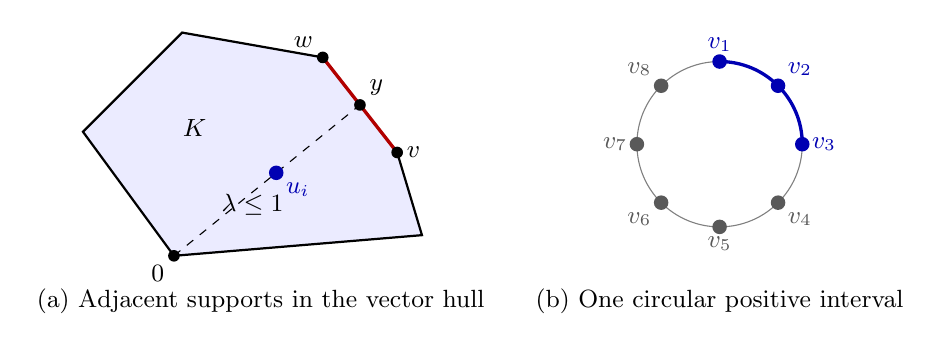
\begin{tikzpicture}[scale=1.05,every node/.style={font=\small}]
  % Query vectors and their adjacent hull supports.
  \fill[blue!8]
    (0,0)--(3,0.25)--(2.7,1.25)--(1.8,2.4)--(0.1,2.7)
    --(-1.1,1.5)--cycle;
  \draw[thick]
    (0,0)--(3,0.25)--(2.7,1.25)--(1.8,2.4)--(0.1,2.7)
    --(-1.1,1.5)--cycle;
  \draw[very thick,red!70!black] (2.7,1.25)--(1.8,2.4);
  \draw[dashed] (0,0)--(2.25,1.825);
  \fill (0,0) circle (2pt) node[below left] {$0$};
  \fill (2.7,1.25) circle (2pt) node[right] {$v$};
  \fill (1.8,2.4) circle (2pt) node[above left] {$w$};
  \fill (2.25,1.825) circle (2pt) node[above right] {$y$};
  \fill[blue!70!black] (1.2375,1.00375) circle (2.5pt)
    node[below right] {$u_i$};
  \node at (0.25,1.55) {$K$};
  \node at (0.95,0.62) {$\lambda\le1$};
  \node[align=center] at (1.05,-0.55)
    {(a) Adjacent supports in the vector hull};

  % A schematic cyclic order; blue vertices form one interval.
  \draw[gray] (6.6,1.35) circle (1);
  \draw[very thick,blue!70!black]
    (6.6,2.35) arc[start angle=90,end angle=0,radius=1];
  \fill[blue!70!black] (6.6,2.35) circle (2.5pt)
    node[above] {$v_1$};
  \fill[blue!70!black] (7.307,2.057) circle (2.5pt)
    node[above right] {$v_2$};
  \fill[blue!70!black] (7.6,1.35) circle (2.5pt)
    node[right] {$v_3$};
  \fill[gray!70!black] (7.307,0.643) circle (2.5pt)
    node[below right] {$v_4$};
  \fill[gray!70!black] (6.6,0.35) circle (2.5pt)
    node[below] {$v_5$};
  \fill[gray!70!black] (5.893,0.643) circle (2.5pt)
    node[below left] {$v_6$};
  \fill[gray!70!black] (5.6,1.35) circle (2.5pt)
    node[left] {$v_7$};
  \fill[gray!70!black] (5.893,2.057) circle (2.5pt)
    node[above left] {$v_8$};
  \node[align=center] at (6.6,-0.55)
    {(b) One circular positive interval};
\end{tikzpicture}
\caption{The first panel depicts normalized query vectors, not
hypotheses: $y$ lies on the edge $vw$ and $u_i=\lambda y$ for
$0<\lambda\le1$. Writing $y=\theta v+(1-\theta)w$ gives
$u_i=\alpha v+\beta w$ with $\alpha+\beta=\lambda\le1$.
Consequently, if both support values on a hypothesis are at most
one, then $u_i\cdot x_h\le1$; equivalently,
$C_i\subseteq C_v\cup C_w$. The second panel shows the cyclic order
only; the positive hull tests of a fixed hypothesis form one
interval in that order.}
\label{fig:support-and-interval}
\end{figure}

\subsection{Interval hitting and discovery length}

\begin{lemma}[Minimum interval cover]\label{lem:minimum-interval-cover}
A minimum-cardinality hitting set for ordinary or circular intervals
on a finite candidate order is computable in polynomial time.
An empty demand is infeasible; an empty family needs no candidates.
\end{lemma}
\begin{proof}
For ordinary intervals, choose the right endpoint $q$ of an
earliest-ending interval $I$. Any cover has a point $u\in I$.
Replacing $u$ by $q$ loses no demand containing $u$: its right
endpoint is at least $q$ and its left endpoint is at most $u\le q$.
Thus an optimal cover can choose $q$. Delete the intervals hit
there and repeat, proving the endpoint greedy rule is exact.

For circular intervals, choose a nonempty demand and enumerate
a forced candidate $v$ in it. Delete demands hit by $v$ and cut
the cycle there. All remaining demands are ordinary intervals,
so use the preceding rule and add $v$. Some forced choice belongs
to an optimal circular cover; take the smallest resulting solution.
\end{proof}

\begin{lemma}[Greedy cover length with adjacent-run credit]
\label{lem:greedy-cover-length}
Let a nonempty family of positively weighted interval demands
be covered by a candidate set $P$ of size $k$. Let $c(P)$ be the
number of runs of consecutive candidates in $P$, measured in the
entire candidate order. Maximum-remaining-weight greedy finishes
within $k+c(P)-1$ choices, for every tie rule.
In particular, a minimum cover of size $k$ gives the usual bound
$2k-1$. For circular intervals the corresponding bound is $2k$.
\end{lemma}
\noindent
The extra term is the number of runs beyond the first. A scattered
cover may force greedy to spend choices repairing several gaps,
whereas a cover arranged in a few contiguous blocks has fewer such
gaps to repair.
\begin{proof}
Induct on $k$. When $k=1$, its sole candidate hits every demand,
and any greedy maximum does so as well.

Let $v$ be the first greedy choice. If it lies at or outside an
extreme of $P$, let $u$ be the nearest extreme cover point.
For example, if $v<\min P=u$, every demand containing $v$ must also
meet $P$, and hence must contain $u$. Thus the demands hit by $v$
are a subset of those hit by $u$. Greedy maximality gives the reverse
inequality on their total weights, so the two candidates hit the
same positive-weight demands.
Thus $P\setminus\{u\}$ covers the remainder, and removing an
extreme does not increase its run count. Induction plus the first
query gives at most $k+c(P)-1$ choices.

Otherwise $v$ lies strictly between the extremes of $P$.
The unhit intervals lie entirely on one side of $v$.
The parts $P_-,P_+$ strictly to its left and right cover these
two families, and
\[
 |P_-|+c(P_-)+|P_+|+c(P_+)\le k+c(P).
\]
If $v\notin P$, cutting in its gap leaves the total run count
unchanged. If $v\in P$, removing it reduces size by one and can
increase total run count by at most one, which proves the displayed
inequality in either case. Greedy may interleave the two sides, but
a choice on one side covers no interval on the other; hence the
choices restricted to either side are still a greedy sequence for
that side. If both families are nonempty,
induction plus the first query gives
\[
 1+\bigl(|P_-|+c(P_-)-1\bigr)
   +\bigl(|P_+|+c(P_+)-1\bigr)\le k+c(P)-1.
\]
If only one is nonempty, the other cover part still has size plus
run count at least two, so the same bound holds. If neither
remains, one query suffices.
Finally $c(P)\le k$, giving $2k-1$ without adjacency information.

For circular intervals, make the first greedy choice and cut the
cycle there. Every unhit interval becomes an ordinary interval.
The original $k$ cover candidates still cover these demands,
so at most $2k-1$ further choices are needed.
\end{proof}

\subsection{Recovering the interval endpoints}
\label{sec:endpoint-geometry}

After discovery, one positive hull vertex $v$ is known.
First inspect its cached neighbor answers. If a neighbor is known
to be negative, cut at that vertex and orient the order so that
$v$ is first. The positive interval starts at $v$, so only its
other endpoint needs a search. If both neighbors are negative,
the pattern consists of $v$ alone and no endpoint query is needed.

Otherwise use a geometric cut. If the origin lies on the hull
boundary, cut at its free negative
marker. If it is interior, the ray from $v$ through $0$ meets
an opposite hull edge with consecutive endpoints $a,b$.
The origin is a convex combination of $v,a,b$, with positive
coefficient on $v$. Thus $a,b$ cannot both be positive: if all
three dot products with $x_h$ exceeded one, their convex
combination would also exceed one, contradicting $0\cdot x_h=0$.
Cut the cyclic order between $a$ and $b$. A circular positive
interval could wrap around this cut only if both endpoints
were positive, which was just excluded. If the ray meets a
vertex, that vertex is necessarily negative and is itself a
free cut point.

No anchor query is made. The positive vertices now form an
ordinary interval containing $v$. To its left, querying a vertex asks whether
the left endpoint is at or before that vertex. To its right,
querying a vertex asks whether the right endpoint is at or after it.
Thus supplied hull queries give exactly the ordered comparisons
needed to locate the two endpoints.



When neither endpoint is already fixed, learn the left endpoint,
then the right endpoint conditioned on
the left endpoint and the earlier transcript. For consecutive
possible left endpoints, querying the earlier endpoint separates
them; for consecutive possible right endpoints, querying the later
endpoint separates them. These are real hull vertices, so all
comparisons used by the codes are supplied queries.
The conditional endpoint distributions come from the hypothesis table.

If $K$ has dimension at most one, it has at most two real vertices.
With two real endpoints, one positive endpoint forces the other
negative because $0$ lies between them. With one real vertex,
its positive bit is the complete nonzero pattern.
Thus no further query is needed in either degenerate case.

A positive discovery exit is \emph{pinned} if a neighbor of its
discovered vertex has a cached negative answer. It is
\emph{singly pinned} when exactly one neighbor is known negative,
and \emph{doubly pinned} when both are. Pinning fixes one or both
endpoints, as described above; it introduces no additional query.

\begin{algorithm}[H]
\caption{\EndpointCode: legal full-pattern recovery}
\label{alg:endpoint-code}
\KwIn{A positive hull vertex $v$, compatible patterns, cached answers;
code mode; optionally fixed continuation heights $h_A$.}
\KwOut{A supplied-query decoder whose leaves are full pattern classes.}
\If{the hull has dimension at most one}{\KwRet the already determined nonzero pattern\;}
\eIf{$v$ has a cached negative neighbor}{
  Cut at that neighbor and orient so $v$ is the first positive vertex\;
}{
  Cut at a boundary origin, or at the opposite edge met by the ray $v0$\;
}
List the realized left and right endpoint pairs in the cut order\;
\eIf{no continuation heights are supplied}{
  Search each unfixed endpoint using Algorithm~\ref{alg:alphabetic-code};
  condition the second search on the first answer\;
}{
  \ForEach{endpoint rectangle $R$, in increasing size}{
    \eIf{$R$ has a single realized class $A$}{$E(R)\gets h_A$\;}{
      $E(R)\gets\min_\ell(1+\max\{E(R\cap\ell^-),E(R\cap\ell^+)\})$,
      over proper supplied endpoint thresholds\;
    }
  }
  Reconstruct the minimizing rectangle splits and attach the fixed child codes\;
}
\KwRet the decoder; skip fixed endpoints and cached thresholds\;
\end{algorithm}

Section~\ref{sec:endpoint-geometry} proves the cut is legal without an
anchor query. With continuation heights this is the complete-exit
optimization of Section~\ref{sec:polynomial-slots}; its $O(M^4)$
rectangles and $O(M)$ thresholds give polynomial running time.


\section{Approximating maximum depth}
\label{sec:worst}

At a balanced state, one query immediately shrinks both child states.
At a flat state, there may be no such query, so the algorithm first
groups hypotheses by their answers to the hull-vertex tests and
then discovers which group contains the target. The two parts of
this work have different roles: the discovery schedule must finish
soon enough for each recursively constructed child code, while the
pattern class must be smaller than the parent. The analysis therefore
uses an optimal path only as a comparison schedule; the algorithm
uses the actual child-code heights when setting its deadlines.

Use the fixed rational count-balance threshold and coefficients
\[
 \delta=\frac{245122334}{10^9},\qquad
 \gamma=\frac{246496526}{10^8},\qquad
 \kappa=3+\gamma=5.46496526.
\]
They satisfy
\begin{equation}\label{eq:worst-parameter-conditions}
 \gamma\log_2\frac1{1-\delta}>1,\qquad
 \gamma\log_2\frac1\delta>5.
\end{equation}
These inequalities pay for balanced queries and flat-state decoding,
respectively. They can be checked with the rational logarithm bounds
in \eqref{eq:rational-log-bounds}.
The probabilities in the expected-depth model are not used by this
algorithm. Write $T_{\mathrm W}(S)$ for the code it constructs on
$S$; its actual height is $c_{\mathrm W}(T_{\mathrm W}(S))$.
In particular, $c_{\mathrm W}(T_{\mathrm W}(\{h\}))=0$.

\begin{symboltable}
$\delta,\ \gamma,\ \kappa$ & Count-balance threshold, coefficient of the logarithmic height credit, and approximation factor.\\
$s,\ D,\ H^*$ & Current state size, its optimum maximum depth, and target height $3D+\lfloor\gamma\log_2s\rfloor$.\\
$t_A,\ g_A$ & First supporting-block index on the comparison path, and actual first-positive position in the constructed schedule.\\
$e_A^{(4)},\ e_A^{(2)}$ & Endpoint-query allowances after a general or second-query positive exit.\\
$u_A,\ B_A,\ d_A$ & Child height plus endpoint allowance, remaining discovery budget under trial height $H$, and support-block deadline.\\
$\mathcal F,\ \mathcal S,\ \mathcal N$ & Classes positive on the first support, first positive on the second support, and negative on both.\\
\end{symboltable}

\subsection{Pattern classes and a height credit}

In a count-flat state $S$, let $s=|S|$ and choose the common witness
$p$ of Lemma~\ref{lem:helly}. Use the normalized hull, patterns,
and support blocks of Definitions~\ref{def:normalized-queries}
and~\ref{def:hull-pattern}.
Lemma~\ref{lem:hull-structure} makes $A_0$ a singleton when present.
Every nonzero class $A$ lies in a supplied minority hull cap, so
\[
 |A|<\delta s.
\]
Write $\Phi(s)=\lfloor\gamma\log_2s\rfloor$. The same integer
credit will pay for the maximum-depth constructions' endpoint exits.
\begin{lemma}[Count-potential credit]\label{lem:worst-floor-credit}
For a balanced child of size $a\le(1-\delta)s$,
$\Phi(s)-\Phi(a)\ge1$. For a flat-state nonzero class of size
$a<\delta s$, put $x=\log_2(s/a)$ and
$\ell=\log_2(1/\delta)$. Then
\begin{equation}\label{eq:worst-floor-credit}
 \Phi(s)-\Phi(a)\ge\lfloor\gamma x\rfloor
 \ge5+\lfloor x-\ell\rfloor.
\end{equation}
\end{lemma}
\begin{proof}
Use $\lfloor u\rfloor-\lfloor v\rfloor\ge\lfloor u-v\rfloor$.
The balanced claim follows from the first inequality in
\eqref{eq:worst-parameter-conditions}. In the flat case $x>\ell$,
and $\gamma\ge1$ and $\gamma\ell>5$ give
$\gamma x>5+(x-\ell)$. Taking floors proves the second claim.
\end{proof}

\begin{lemma}[Pathwise supporting-prefix credit]\label{lem:height-prefix}
Fix a proper maximum-depth-optimal tree for $S$, of height
$D=\OPT_{\mathrm W}(S)$, and follow $p$ along its path
$Q=(i_1,\ldots,i_q)$ to leaf $z$.
For a pattern class $A$, let $t_A$ be the first index whose
supporting hull vertices include a positive vertex of $A$;
put $t_A=q+1$ if there is no such index. Then
\[
 \OPT_{\mathrm W}(A)\le \OPT_{\mathrm W}(S)-(t_A-1).
\]
There is a comparison sequence of support blocks, each a singleton
or an adjacent pair of real hull vertices, covering every nonzero
pattern in its first $t_A$ blocks.
\end{lemma}
\begin{proof}
Before $t_A$, all supporting hull bits of each path query are zero
on the whole class. Convexity forces the original query's frozen
answer throughout $A$. Thus every member follows the same first
$t_A-1$ queries, and restriction to $A$ contracts all of them.
Every original path has length at most $D$, proving the height bound.
This is the height credit: the class can afford a longer search for
its pattern only to the extent that its common prefix has already
disappeared from the restricted optimal tree.

Replace each query of $Q$ by its block of real supporting
hull vertices. A class with $t_A\le q$ is covered in block $t_A$.
A class with no supporting hit follows the entire original path
and must be the singleton $\{z\}$. If that pattern is nonzero,
append one of its positive hull vertices as block $q+1$.
Repeated supports are harmless. If the pattern is zero, it is the
terminal core and needs no positive hit.
\end{proof}

\subsection{A pointwise pattern-decoding allowance}

Once a positive hull answer is known, the pattern can be recovered
by the endpoint method of Section~\ref{sec:endpoint-geometry}.
For the worst-case algorithm use the explicit midpoint-dyadic
alphabetic code in Lemma~\ref{lem:alphabetic-endpoints}, not a tree
chosen merely for minimum expected depth.
The code-design probabilities are uniform counts on $S$, conditioned
on the observed transcript; they do not represent randomization of
the algorithm.

\begin{lemma}[Per-class endpoint allowance]\label{lem:endpoint-height}
After the first positive answer, every hypothesis in a nonzero
class $A$, of size $a$, needs at most
\[
 e_A^{(4)}=\left\lfloor\log_2\frac{\delta s}{a}\right\rfloor+4
\]
additional queries to recover the full pattern.
If an adjacent hull vertex is already known to be negative, the
allowance improves to
\[
 e_A^{(2)}=\left\lfloor\log_2\frac{\delta s}{a}\right\rfloor+2.
\]
There is no additional query on the zero-pattern route once the
other patterns have been covered.
\end{lemma}
\begin{proof}
The opposite-edge cut in Section~\ref{sec:endpoint-geometry} makes
the positive pattern an ordinary interval without querying a
negative anchor. Its two endpoints are learned by supplied hull
thresholds.

Let $R$ be the compatible set after the first positive answer.
It lies in the positive hull cap, so $|R|<\delta s$.
The auxiliary uniform distribution on $S$ is uniform on $R$,
and all of $A$ remains compatible.
If $a_L$ members of $R$ have the target's left endpoint, the two
explicit alphabetic codes use at most
\[
 \log_2\frac{|R|}{a_L}+2
 +\log_2\frac{a_L}{|A|}+2
 =\log_2\frac{|R|}{a}+4
 <\log_2\frac{\delta s}{a}+4
\]
queries on that target. The second probability is conditioned on
the first endpoint. Their pair uniquely specifies its pattern.
Each of the two alphabetic searches contributes the additive $2$
in its pointwise code bound; multiplying the two conditional
probabilities makes their logarithmic terms telescope to
$\log_2(|R|/a)$.
The number of queries is an integer, so the displayed upper bound
implies the stated floor-based allowance.
If a negative vertex is adjacent to the positive one, cut at that
negative vertex and choose the orientation in which the positive
one is first. The positive interval must start there, so one
endpoint is fixed. A single alphabetic code learns the other
endpoint and uses at most
$\log_2(|R|/a)+2<\log_2(\delta s/a)+2$ queries.
This gives the second allowance. The actual negative answer is
the cut marker; no opposite-edge query or assumption about the
origin's location is required on this route.
In a hull of dimension at most one, the positive pattern is already
determined after discovery.
Singleton inference and cached answers only reduce the allowance.
\end{proof}

The next observation separates the local height test, which the
algorithm can check, from the optimal-path comparison used later.
\begin{lemma}[Local route-height test]\label{lem:worst-local-height}
Suppose each full pattern class $A$ has a stored identifying code
of actual height $h_A$. Discover a positive vertex using a fixed
ordering, truncated when every nonzero pattern is covered, and then
recover its full pattern. If $g_A$ is the first positive position,
the complete route through $A$ has height at most
\[
 g_A+h_A+e_A^{(4)},
\]
or $g_A+h_A+e_A^{(2)}$ when a negative neighbor is already cached.
If all these bounds are at most $H$, the entire tree has height at
most $H$, including the zero-pattern route when present.
\end{lemma}
\begin{proof}
The route consists of discovery, endpoint recovery, and the stored
child code; Lemma~\ref{lem:endpoint-height} bounds its middle part.
The all-negative route has length $\max_{A\ne A_0}g_A\le H$ and
ends at the zero singleton. An absent zero class creates no leaf.
For a nonsingleton state there is at least one nonzero pattern,
since $|A_0|\le1$.
\end{proof}

\subsection{Priority greedy with an enumerated adjacent pair}

The comparison path gives a deadline for every pattern class, but
the algorithm does not know that path. It must produce one ordering
that meets all deadlines at once. Enumerating the first adjacent
pair fixes the circular cut; priority weights then make ordinary
maximum-remaining-weight greedy behave like greedy for every
deadline prefix, without requiring the comparison blocks as input.

The indices $t_A,d_A$ count support blocks; $g_A$ counts actual
vertex queries. The scheduler translates a feasible block deadline
into a bound on that actual first-positive position.

\begin{lemma}[Adjacent-block schedule]\label{lem:deadline-cover}
Fix two distinct adjacent hull vertices $v,w$ and consider the
pattern classes negative on both. Assign each such class an integer
block budget $d_A\ge2$. Suppose a comparison sequence of support
blocks starts with $\{v,w\}$, every other block is empty, a singleton,
or an adjacent pair, and it hits $A$ in its first $d_A$ blocks.

Force $v,w$ along the negative discovery route. Give a class of
budget $d^{(j)}$ the auxiliary integer weight $M^{r-j}$, where
$d^{(1)}<\cdots<d^{(r)}$ are the distinct budgets and $M=s+1$.
Then complete discovery by maximum-remaining-weight greedy.
In this one ordering every surviving class satisfies
\[
 g_A\le3d_A-2.
\]
The schedule and its first-hit times are computable in polynomial
time without knowing the comparison blocks.
\end{lemma}
\begin{proof}
Fix a budget $d=d^{(j)}$ and restrict demands to the prefix
$\mathcal P_j=\{A:d_A\le d\}$. Every score from these demands
is an integer multiple of $M^{r-j}$. The total weight of all later
demands is less than $M^{r-j}$: there are at most $s$ classes and
each later weight is at most $M^{r-j-1}$, with $s<M$.
When there are no later demands this weight is zero.

The weight of one prefix hit therefore outweighs every possible
contribution from later-deadline classes. Thus later demands cannot
reverse a strict comparison of prefix scores. After the forced pair,
until the prefix is covered,
each global greedy choice
is a weighted greedy choice for its remaining prefix demands.
It hits at least one of them; a zero prefix score cannot beat a
positive prefix score. Ties may use later weights but are legitimate
greedy ties for the prefix.

Cut at $v$ and delete $w$. The remaining demands are ordinary
intervals. Because the removed vertices were adjacent, every
comparison pair avoiding them is still consecutive in this linear
candidate order; a block meeting them becomes at most a singleton.
Let $P$ be the union of the first $d$ comparison blocks with $v,w$
removed, and let $c(P)$ count its runs of consecutive candidates.
The first block contributes nothing. Each later block contributes
at most three to size plus run count: an adjacent pair has size two
and one run, while a singleton has size one and one run. Both
quantities are subadditive under union, so
\[
 |P|+c(P)\le3(d-1).
\]
This set covers the surviving prefix. For any nonempty surviving
prefix, its classes are negative on $v,w$ and therefore must be hit
in a later comparison block, so $P$ is nonempty.
If it is nonempty,
Lemma~\ref{lem:greedy-cover-length} bounds the number of additional
greedy choices by $|P|+c(P)-1\le3d-4$.
Including the forced pair gives $3d-2$.
The priority argument applies to every prefix in the same ordering.

The auxiliary weights have $O(s\log s)$ bits, and greedy only sums
and compares them using the explicit class-to-vertex incidence
table. The block budgets are internal scheduling quantities, not
additional constraints in the identification problem.
\end{proof}

\begin{algorithm}[H]
\caption{\PriorityTrial: one height trial with stored child codes}
\label{alg:priority-trial}
\KwIn{Flat state's hull and classes; child heights $h_A$; allowances $e_A^{(4)},e_A^{(2)}$; target $H$.}
\KwOut{A passing discovery order, or infeasible.}
\ForEach{oriented adjacent real pair $(v,w)$}{
  Form $\mathcal F,\mathcal S,\mathcal N$ by their first hit on $(v,w)$\;
  \If{some $A\in\mathcal F$ has $1+h_A+e_A^{(4)}>H$, or
  some $A\in\mathcal S$ has $2+h_A+e_A^{(2)}>H$}{\Continue\;}
  \ForEach{$A\in\mathcal N$}{
    $u_A\gets h_A+e_A^{(4)}$;
    $B_A\gets H-u_A$;
    $d_A\gets\lfloor(B_A+2)/3\rfloor$\;
  }
  \If{some $B_A<4$}{\Continue\;}
  Sort distinct budgets as $d^{(1)}<\cdots<d^{(r)}$\;
  Give each deadline-$d^{(j)}$ class weight $(|S|+1)^{r-j}$\;
  Force $v,w$ and complete by maximum-remaining-weight greedy;
  truncate when all nonzero classes are hit\;
  \If{every $A\in\mathcal N$ has actual $g_A+u_A\le H$}{\KwRet this order\;}
}
\KwRet infeasible\;
\end{algorithm}


\subsection{The recursive maximum-depth algorithm}

Algorithms~\ref{alg:priority-trial} and~\ref{alg:worst-tree} give the
explicit construction. At a balanced state query a balanced line and
recurse. At a flat state build every pattern child \emph{before}
scheduling; the trial uses its actual height, not its optimum. For an
oriented initial pair $(v,w)$, the first-positive classes satisfy the
direct one-query and two-query height checks. For classes negative on
both, put
\[
 u_A=c_{\mathrm W}(T_{\mathrm W}(A))+e_A^{(4)},\qquad
 B_A=H-u_A,\qquad d_A=\lfloor(B_A+2)/3\rfloor.
\]
Reject if $B_A<4$, then use the priority weights of
Lemma~\ref{lem:deadline-cover} and accept only if each actual first hit
satisfies $g_A+u_A\le H$. Trial heights range from one through
$\lfloor\kappa(s-1)\rfloor$.

After a positive answer, Algorithm~\ref{alg:endpoint-code} learns the
full pattern and the stored child identifies its hypothesis. The
second-query exit has a cached negative neighbor and uses only one
endpoint code. Stop discovery as soon as all nonzero patterns are
covered; its all-negative route identifies $A_0$ when present and is
omitted otherwise. Low-dimensional hulls use their extreme tests
directly. Every nonsingleton pattern child is smaller, so the recursion
is well founded.

Lemma~\ref{lem:worst-local-height} makes a passing trial a complete
height certificate. Its first two exits have discovery costs one
and two, respectively; the latter has a cached negative neighbor.
Every remaining class uses the general allowance. The checks use
the explicit schedule's actual first-hit times.

\begin{algorithm}[H]
\caption{\WorstTree: the priority maximum-depth baseline}
\label{alg:worst-tree}
\KwIn{State $S$ and the rational parameters of Section~\ref{sec:worst}.}
\KwOut{A supplied-query identification tree.}
\If{$|S|\le1$}{\KwRet its leaf\;}
\If{a count-balanced supplied line $\ell$ exists}{
  \KwRet $\ell$ with recursively constructed children $\WorstTree(S_\ell^-)$ and $\WorstTree(S_\ell^+)$\;
}
Compute $\HullData(S)$ and recursively build one child $T_A$ per pattern class\;
\If{the hull has at most two real extreme vertices}{
  \KwRet their direct pattern stage with the stored children attached\;
}
Compute $e_A^{(4)},e_A^{(2)}$ from Lemma~\ref{lem:endpoint-height}\;
\For{$H=1,\ldots,\lfloor(3+\gamma)(|S|-1)\rfloor$}{
  $Q\gets\PriorityTrial(S,(c_W(T_A)),(e_A^{(4)},e_A^{(2)}),H)$\;
  \If{$Q$ is feasible}{
    Build its first-positive exits, use pointwise $\EndpointCode$ at each exit,
    and attach the stored class children\;
    End the all-negative route at the zero singleton when present\;
    \KwRet this tree\;
  }
}
\end{algorithm}


\begin{theorem}[Constant deterministic maximum-depth approximation]
\label{thm:worst}
The preceding polynomial-time deterministic algorithm satisfies
\[
 c_{\mathrm W}(T_{\mathrm W}(S))\le
 3\OPT_{\mathrm W}(S)+\left\lfloor\gamma\log_2|S|\right\rfloor
 \le\kappa\OPT_{\mathrm W}(S),\qquad \kappa=5.46496526<5.464966.
\]
It uses only supplied line queries.
\end{theorem}
\begin{proof}
Induct on $s=|S|$, with a zero-cost singleton, and write
$D=\OPT_{\mathrm W}(S)$ and $H^*=3D+\lfloor\gamma\log_2s\rfloor$.
A balanced child has size $a\le(1-\delta)s$ and optimum at most $D$,
so Lemma~\ref{lem:worst-floor-credit} pays for its root query.

In a flat state put $L_A=\log_2(s/|A|)$ and
$\ell=\log_2(1/\delta)$.

Choose an enumerated initial pair containing the first optimal-witness
query's supports; pad a singleton support with an adjacent real
neighbor. This only adds coverage. The inductive bound and
\eqref{eq:worst-floor-credit} leave at least one query after the
general endpoint allowance, and at least three after the singly pinned
allowance. Thus the first and second positive exits pass their direct
height checks, including classes hit by the padding.

For a class $A$ negative on both first supports, its comparison index
has $t_A\ge2$. Lemma~\ref{lem:height-prefix} and induction give
\[
\begin{aligned}
 B_A=H^*-u_A
 &\ge3(t_A-1)+\lfloor\gamma L_A\rfloor
                    -\lfloor L_A-\ell\rfloor-4\\
 &\ge3t_A-2\ge4.
\end{aligned}
\]
Hence $d_A=\lfloor(B_A+2)/3\rfloor\ge t_A$. The padded first block,
the original supporting blocks, and the terminal nonzero singleton
block when needed satisfy Lemma~\ref{lem:deadline-cover}. Its single
priority ordering therefore obeys
\[
 g_A\le3d_A-2
 =3\lfloor(B_A+2)/3\rfloor-2\le B_A.
\]
The last inequality follows by writing $B_A+2=3d_A+r$ with
$r\in\{0,1,2\}$. All actual-height checks pass. Truncating at the
last positive first hit also puts the zero singleton within $H^*$.
A one-dimensional hull needs at most two extreme tests; its count
potential drop pays for these directly.

Thus the least passing trial has height at most $H^*$. Since
$\log_2s\le D\le s-1$, this integer trial lies in the prescribed
range and $H^*\le(3+\gamma)D$. No optimum is queried by the algorithm.
\end{proof}

The bound controls the longest path of one deterministic output
tree, not an expected query count over random trees.
There are at most $n-1$ nonterminal stages. A flat stage tries
$O(s)$ integer bounds, each trying at most $2|V|$ oriented adjacent
pairs and a weighted greedy completion.
The endpoint code-design probabilities are counts, so
the explicit alphabetic codewords have $O(\log s)$ bits.
Geometry, child-height evaluation, schedule checks, and decoding-code
construction all have polynomial bit complexity.
The proper complete output tree has $n-1$ internal nodes.

The two parameter constraints explain the optimized threshold.
For this induction, the least possible coefficient is
\[
 \gamma(\delta)=
 \max\left\{\frac1{\log_2(1/(1-\delta))},
             \frac5{\log_2(1/\delta)}\right\}.
\]
The first term decreases with $\delta$ and the second increases,
so their maximum is minimized where they are equal. Solving this
equation gives $\delta=(1-\delta)^5$, at approximately
$0.2451223337533$.
The chosen rational parameters give a factor within $5\cdot10^{-9}$
of the resulting minimum $5.4649652555$.
The first pair also serves two purposes: it removes one support
block from the greedy coverage bound, and its second-query exit is
singly pinned, so only one endpoint code is needed.

\section{Scheduling the first positive answer}
\label{sec:scheduling}

The maximum-depth algorithm schedules discovery around the heights
of its child codes. For expected depth, a cap containing a likely
target should instead be encountered early. This is a weighted min-sum set cover (MSSC) problem. The sets remain
the supplied caps;
singleton sets are not added unless an actual supplied test realizes
them.

In the decision-tree application, a positive hull answer exits the
all-negative route and reveals that the target lies in a small cap.
The all-zero pattern has no positive answer, so on the full-cover
route it is identified after every positive pattern has been covered
(and an earlier singleton inference only shortens that route). Its
contribution is therefore at most its weight times the schedule
length. This is why the
ordering analysis keeps both the first-cover sum and a separate
length term.

\begin{symboltable}
$U,\ \pi_h,\ p_0$ & Coverable positive-pattern demands, their positive weights, and the weight of a target found only after the schedule finishes.\\
$t_Q(h),\ \MSSC(Q)$ & First-cover position of demand $h$ in ordering $Q$ and the sum $\sum_h\pi_h t_Q(h)$.\\
$k_0$ & Minimum number of candidate tests needed to cover all demands in $U$.\\
$\beta,\ \Phi_\beta,\ Z_\beta$ & Geometric budget factor and the first-cover and total-length accounting functions.\\
$r_Q(x),\ G_u$ & Comparison-order mass with first-cover time greater than $x$, and the constructed schedule for shift $u$.\\
\end{symboltable}

For background, weighted MSSC has a classical greedy
four-approximation~\cite{flt2004}. We do not use that guarantee in
either proof. Instead, exact coverage with a cardinality budget
gives the stronger circular-interval ordering proved below,
including a bound on its total length.

\begin{lemma}[Exact budgeted interval coverage]\label{lem:budget-coverage}
For positively weighted interval or circular-interval demands on
a finite candidate set, a set of at most $k$ candidates hitting
maximum demand weight is computable in polynomial time.
\end{lemma}
\begin{proof}
Algorithm~\ref{alg:interval-cover} gives both interval oracles.
For ordinary intervals, number the candidates $1,\ldots,M$.
If the previous selected candidate is $p$ and the next is $q>p$,
the newly hit demands are exactly the intervals containing $q$
whose left endpoint is greater than $p$. An interval containing
$q$ and an earlier selected point must also contain $p$.
Conversely, any interval containing $q$ with left endpoint greater
than $p$ contains no earlier selected candidate. Thus the added
weight $g(p,q)$ depends only on these two positions, not on the
earlier choices.

For exactly $t$ selected candidates ending at $q$, use the recurrence
\[
 D(t,q)=\max_{p<q}\{D(t-1,p)+g(p,q)\},
 \qquad D(0,0)=0.
\]
The position $0$ is a \emph{sentinel}, an artificial initial marker
before every interval, not a selectable candidate.
All other zero-candidate or nonexistent states are infeasible
and have value $-\infty$ in this maximization.
Take the maximum over
$t\le k$ and final positions, including the empty selection.
This is a polynomial dynamic program.

For circular intervals and $k\ge1$, enumerate a selected candidate
$v$. Credit the demands it hits and delete them. Cutting at $v$
turns the remaining demands into ordinary intervals, on which
the dynamic program selects at most $k-1$ more candidates.
One enumeration contains a candidate of an optimal nonempty
selection, so taking the best is exact. The $k=0$ case is empty.
\end{proof}

\begin{algorithm}[H]
\caption{\IntervalCover: exact minimum cover or budgeted coverage}
\label{alg:interval-cover}
\KwIn{Ordered interval demands with weights; either \emph{minimum} or budget $k$;
ordinary or circular order.}
\KwOut{A minimum hitting set, or a maximum-weight set of size at most $k$.}
\If{order is circular}{
  Enumerate a forced selected candidate $v$; delete its hit demands and cut there\;
  Solve each residual ordinary instance, with budget $k-1$ in budget mode\;
  \KwRet the best residual solution plus $v$, also considering the empty budget solution\;
}
\eIf{mode is \emph{minimum}}{
  \If{an empty demand exists}{\KwRet infeasible\;}
  $P\gets\varnothing$\;
  \While{a demand remains}{
    Choose the right endpoint $q$ of an earliest-ending remaining demand\;
    $P\gets P\cup\{q\}$; delete all demands containing $q$\;
  }
  \KwRet $P$\;
}{
  Set $D(0,0)=0$ and all other unreachable states to $-\infty$\;
  Precompute $g(p,q)$: weight of intervals containing $q$ with left endpoint $>p$\;
  \For{$t=1,\ldots,\min\{k,M\}$}{
    \For{$q=1,\ldots,M$}{
      $D(t,q)\gets\max_{p<q}(D(t-1,p)+g(p,q))$; store a maximizing $p$\;
    }
  }
  \KwRet the reconstruction of the best state with $t\le k$, including $(0,0)$\;
}
\end{algorithm}

For minimum circular cover the forced candidate need only range over
one nonempty demand. For budget coverage, empty demands contribute
zero covered weight. The empty family returns the empty set in both
modes. Lemmas~\ref{lem:minimum-interval-cover} and
\ref{lem:budget-coverage} establish exactness.


The next lemma uses exact budgeted covers at geometrically
increasing budgets. Small budgets can discover likely targets early;
the minimum cover at the final budget guarantees that every positive
target is eventually found. Shifting the budget sequence changes
where it crosses integer thresholds. Averaging over shifts bounds
both positive first-cover times and the zero-pattern waiting time;
a finite search over the distinct resulting schedules removes the
random shift.

\begin{lemma}[Geometric-batch ordering]\label{lem:mssc}
Let $U$ be a nonempty family of coverable weighted circular intervals.
Let $k_0$ be its minimum cover size and let $p_0\ge0$ be the weight
of a target covered only when the entire schedule finishes.
Fix rational $\beta>1$, and put
\[
 r_\beta=\lfloor\beta\rfloor,\qquad
 \lambda_\beta=\frac{\beta+1}{2\ln\beta},\qquad
 \nu_\beta=1+\frac1{\ln\beta},\qquad
 \eta_\beta=\frac{r_\beta+1}{2}
            -\frac{\ln(r_\beta!)}{2\ln\beta}-\lambda_\beta.
\]
For integer $t,k\ge1$, define the accounting functions
\[
 \begin{aligned}
 \Phi_\beta(t)
 &=\lambda_\beta+\eta_\beta
    +\frac1{2\ln\beta}\int_1^t
       \frac{\lfloor x\rfloor+\lfloor\beta x\rfloor}{x}\,dx,\\
 Z_\beta(k)
 &=k+\frac{k\ln k-\ln(k!)}{\ln\beta}.
 \end{aligned}
\]
A deterministic polynomial-time ordering $G$ satisfies, for every
comparison cover ordering $Q$,
\[
 \MSSC(G)+p_0|G|
 \le\sum_{h\in U}\pi_h\Phi_\beta(t_Q(h))+p_0 Z_\beta(k_0).
\]
The simpler bounds
$\Phi_\beta(t)\le\lambda_\beta t+\eta_\beta$ and
$Z_\beta(k)\le\nu_\beta k-1/\ln\beta$ also hold.
Every candidate schedule considered by the construction also has
length at most $\bigl(1+\beta/(\beta-1)\bigr)k_0$.
\end{lemma}
\begin{proof}
Compute a minimum cover $Q_*$ using
Lemma~\ref{lem:minimum-interval-cover} and, for each integer $k<k_0$,
an exact maximum-weight coverage set $Q_k$ of at most $k$
candidates using Lemma~\ref{lem:budget-coverage}.
Fix the selected sets deterministically.

Fix a comparison cover ordering $Q$, and write
\[
 r_Q(x)=\sum_{h:t_Q(h)>x}\pi_h
\]
for the weight whose first-cover index in $Q$ exceeds $x$.
For a shift $u\in[1,\beta)$, use budgets
$k^{(j)}=\lfloor\beta^ju\rfloor$, $j=0,1,\ldots$.
In each phase, process $Q_{k^{(j)}}$ when $k^{(j)}<k_0$ and $Q_*$
otherwise. Order that set greedily by the weight it covers among
the demands still unhit by earlier queries. Omit repeated queries
and those hitting no remaining demand. Stop after the first phase
whose budget reaches $k_0$.
\begin{claim}[Phase coverage and schedule length]
After a phase with budget $k<k_0$, the weight still unhit is at
most $r_Q(k)$. The complete shifted schedule has length at most
$\bigl(1+\beta/(\beta-1)\bigr)k_0$.
\end{claim}
\begin{proof}
The union of all queries processed through this phase covers every
demand covered by $Q_k$: a query omitted for hitting no remaining
demand has its covered demands already hit by an earlier phase.
The set $Q_k$ covers at least as much total weight as the first
$k$ queries of $Q$, since those queries are one feasible
at-most-$k$ candidate set. Hence the schedule has hit at least the
weight hit by that comparison prefix, leaving at most $r_Q(k)$.
The final $Q_*$ phase covers all demands.

Let $J$ be the first phase whose budget reaches $k_0$. The
pre-final phases use at most
\[
 \sum_{j<J}\lfloor\beta^ju\rfloor
 <\sum_{j<J}\beta^ju
 <\frac{\beta}{\beta-1}k_0
\]
queries: the last pre-final unrounded budget is below $k_0$, and
the preceding terms decrease geometrically by a factor $1/\beta$.
The final minimum cover uses $k_0$ queries, proving the length
bound.
\end{proof}

\begin{claim}[First-cover cost within one batch]
Suppose a phase processes $m$ queries, newly hitting weights
$g_1,\ldots,g_m$ in order, and starts and ends with unhit weights
$r$ and $r'$. Its contribution to the first-cover sum is at most
\[
 mr'+\sum_{i=1}^m i g_i
 \le mr'+\frac{m+1}{2}(r-r')
 =\frac{m+1}{2}r+\frac{m-1}{2}r'.
\]
\end{claim}
\begin{proof}
After each greedy choice, the remaining coverage of every unused
candidate can only decrease. Therefore the newly hit weights are
nonincreasing: $g_1\ge\cdots\ge g_m$. Pairing ranks $i$ and
$m+1-i$ shows
\[
 \sum_{i=1}^m i g_i\le\frac{m+1}{2}\sum_{i=1}^m g_i.
\]
Indeed, in each pair the earlier rank has at least as much weight
as the later one, so replacing both ranks by their mean cannot
decrease the weighted sum. A demand first hit at rank $i$ remains
unhit for exactly $i$ queries in this batch, while each demand
still unhit at the end remains unhit for all $m$ queries. Since
$\sum_i g_i=r-r'$, their combined contribution gives the claim.
\end{proof}

Now let $r_j$ be the unhit weight after phase $j$, and put
$r_{-1}=w(U)$. If phase $j$ processes $m_j$ queries, the preceding
claim bounds its first-cover contribution by
\[
 \frac{m_j+1}{2}r_{j-1}+\frac{m_j-1}{2}r_j.
\]
Since $m_j\le k^{(j)}$, replacing $m_j$ by its integer budget and
combining adjacent phase coefficients gives
\[
 \MSSC(G_u)\le
 \frac{\lfloor u\rfloor+1}{2}w(U)
 +\frac12\sum_{j\ge0}
       \bigl(k^{(j)}+k^{(j+1)}\bigr)r_Q(\beta^ju).
\]
For every pre-final phase, the first claim gives
$r_j\le r_Q(k^{(j)})=r_Q(\beta^ju)$; the equality uses the
integer-valued comparison first-cover indices. The final phase
has residual zero. The displayed infinite sum only adds
nonnegative upper bounds for the final and later phases.

\paragraph{Average the first-cover cost.}
Average this expression over a \emph{log-uniform shift}, with
probability density $1/(u\ln\beta)$ on $[1,\beta)$. This density
integrates to one because $\int_1^\beta du/u=\ln\beta$.
Splitting the first term's integral at its integers
gives
\[
 \begin{aligned}
 \mathbb E[\lfloor u\rfloor]
 &=\frac{\displaystyle
     \sum_{k=1}^{r_\beta-1}k\ln\frac{k+1}{k}
        +r_\beta\ln\frac{\beta}{r_\beta}}{\ln\beta}\\
 &=r_\beta-\frac{\ln(r_\beta!)}{\ln\beta}.
 \end{aligned}
\]
The intervals $[\beta^j,\beta^{j+1})$ partition $[1,\infty)$,
so averaging the remaining terms gives
\[
 \begin{aligned}
 \mathbb E[\MSSC(G_u)]
 &\le(\lambda_\beta+\eta_\beta)w(U)\\
 &\quad+\frac1{2\ln\beta}\int_1^\infty
      \frac{\lfloor x\rfloor+\lfloor\beta x\rfloor}{x}
      r_Q(x)\,dx\\
 &=\sum_{h\in U}\pi_h\Phi_\beta(t_Q(h)).
 \end{aligned}
\]
For each real $x$, write
$r_Q(x)=\sum_{h:t_Q(h)>x}\pi_h$. Interchanging this finite sum
with the integral makes each hypothesis contribute the integral
from $1$ to its integer first-cover time. Adding the initial
$(\lambda_\beta+\eta_\beta)w(U)$ term gives exactly
$\sum_{h\in U}\pi_h\Phi_\beta(t_Q(h))$.
Bounding the integrand by $\beta+1$ recovers
$\Phi_\beta(t)\le\lambda_\beta t+\eta_\beta$, but would discard
the savings from all later integer budgets.

\begin{claim}[Shift-averaged schedule length]
Under the same shift distribution,
\[
 \mathbb E[|G_u|]\le Z_\beta(k_0)
 \le\nu_\beta k_0-\frac1{\ln\beta}.
\]
\end{claim}
\begin{proof}
The final cover contributes $k_0$ queries. The earlier phases
contribute at most
$\sum_{j:\,\beta^ju<k_0}\lfloor\beta^ju\rfloor$.
After averaging and substituting $x=\beta^ju$, their expected
length is
\[
 \frac1{\ln\beta}\int_1^{k_0}\frac{\lfloor x\rfloor}{x}\,dx.
\]
On each interval $[j,j+1)$, $\lfloor x\rfloor=j$, so summing the
integrals gives
\[
 \int_1^{k_0}\frac{\lfloor x\rfloor}{x}\,dx
 =k_0\ln k_0-\ln(k_0!).
\]
Consequently $\mathbb E[|G_u|]\le Z_\beta(k_0)$. Since $\ln x$
is increasing,
\[
 \ln(k_0!)=\sum_{j=2}^{k_0}\ln j
 \ge\int_1^{k_0}\ln x\,dx
 =k_0\ln k_0-k_0+1.
\]
Substituting this in $Z_\beta(k_0)$ gives
$Z_\beta(k_0)\le\nu_\beta k_0-1/\ln\beta$. The formula also gives
$Z_\beta(1)=1$.
\end{proof}

The first-cover and length bounds hold under the same shift
distribution. Therefore
\[
 \mathbb E[\MSSC(G_u)+p_0|G_u|]
 \le\sum_{h\in U}\pi_h\Phi_\beta(t_Q(h))
      +p_0Z_\beta(k_0).
\]

No random shift is used by the algorithm. Let $J$ be the first
integer with $\beta^J\ge k_0$. All budget changes occur at the
rational breakpoints $u=k/\beta^j$ for
$0\le j\le J$, $1\le k\le k_0$, inside $[1,\beta)$.
Enumerate these breakpoints and one rational midpoint between
each consecutive pair, construct the resulting orderings, and
take the one minimizing the rational quantity
$\MSSC(G_u)+p_0|G_u|$. There are
$O(k_0\log k_0)$ intervals for fixed $\beta$.
The budgets, selected sets, and their greedy internal orders are
constant on each interval. Their minimum joint value is at most
the average just bounded. The waiting-time weight $p_0$ is used
only to choose the schedule; all queries remain supplied candidates.
\end{proof}

\begin{algorithm}[H]
\caption{\BatchOrders: deterministic family of geometric-batch schedules}
\label{alg:batch-orders}
\KwIn{Weighted circular demands and rational $\beta>1$.}
\KwOut{All schedules needed for deterministic shift minimization.}
Compute a minimum cover $Q_*$ of size $k_0$ using $\IntervalCover$\;
\For{$k=1,\ldots,k_0-1$}{Compute a maximum-weight budget-$k$ set $Q_k$\;}
Find the first $J$ with $\beta^J\ge k_0$ by rational multiplication\;
Form the breakpoints $1,\beta$ and $k/\beta^j\in[1,\beta)$,
$0\le j\le J$, $1\le k\le k_0$\;
\ForEach{breakpoint below $\beta$ and each midpoint of consecutive breakpoints}{
  $u\gets$ that rational representative; $Q\gets$ empty order\;
  \For{$j=0,1,\ldots$}{
    $k\gets\lfloor\beta^ju\rfloor$;
    $P\gets Q_k$ if $k<k_0$, and $P\gets Q_*$ otherwise\;
    Greedily order $P$ by newly covered weight, append its productive unused candidates to $Q$\;
    \If{$k\ge k_0$}{stop this shift's phases\;}
  }
  Retain $Q$\;
}
\KwRet the retained family, removing duplicate schedules\;
\end{algorithm}

An empty demand family needs no schedule. Lemma~\ref{lem:mssc}
bounds the family's minimum joint first-cover and waiting cost.
The number of representatives is $O(k_0\log k_0)$ for fixed $\beta$.


\section{A constant approximation for expected depth}
\label{sec:mass-improvement}

The expected-depth algorithm distinguishes balanced and flat states
by probability mass. Like the maximum-depth algorithm, it learns
the complete hull pattern before recursing. Its discovery ordering
uses exact weighted coverage rather than the heights of child codes.
The proof uses the same three steps in this section and in all later
expected-depth improvements: compare discovery with queries deleted
from an optimal witness path; bound the information still needed to
recover the full pattern; then telescope these two local credits.
Lemma~\ref{lem:stage-conversion} performs the last step once for all
variants. The algorithm itself uses only coverage, endpoint codes, and
rational scores; the witness path and information quantities are proof
objects.
Fix
\[
 \beta=\frac{3512863}{10^6},\qquad
 \lambda=\frac{\beta+1}{2\ln\beta},\qquad
 \nu=1+\frac1{\ln\beta},
\]
and the accounting coefficients
\[
 A_\beta=2\lambda,\qquad
 C_\beta=\frac{\Phi_\beta(1)+\Phi_\beta(2)}2,\qquad
 B_\beta=4+C_\beta.
\]
For this $\beta$, $\lfloor\beta\rfloor=3$ and
$\lfloor2\beta\rfloor=7$. Splitting the integrals at their integer
breakpoints gives
\[
 C_\beta=3-\frac{\ln(945/8)}{4\ln\beta},\qquad
 B_\beta=7-\frac{\ln(945/8)}{4\ln\beta}.
\]
The chosen $\beta$ satisfies $\lambda>\nu$.

Revealing a pattern makes an initial segment of an optimal witness
path unnecessary; those deleted queries pay for its discovery.
Entropy pays for the pattern information that remains. We seek a
local bound of the form
\[
 \text{expected queries in a stage}
 \ \le\ A_\beta\Delta_{\mathrm E}(S,\Pi)+cI(S,\Pi)
\]
for a constant $c$ and the stage's output partition $\Pi$.
Unlike a bound proportional to $\OPT_{\mathrm E}(S)$ alone, this inequality sums
over nested states without charging the same optimum repeatedly.

\subsection{Hull tests and their answer patterns}

Fix a strict test witness $p$ and use the common notation of
Definitions~\ref{def:normalized-queries} and~\ref{def:hull-pattern}.
These hull vertices are used for discovery, not as a replacement for
the original query family. Once the pattern class is known, the
recursive algorithm again has access to every supplied line.

Lemma~\ref{lem:hull-structure} gives cap coverage and interval
patterns. Lemma~\ref{lem:mssc} gives a deterministic ordering with
latency and length bounds. Endpoint recovery is described in
Section~\ref{sec:endpoint-geometry}.

\subsection{The queries a pattern makes unnecessary}

\begin{lemma}[Supporting-prefix credit]\label{lem:support-prefix}
Let $T^*$ be an expected-depth-optimal proper tree for $S$.
Follow $p$ through it, with queries $Q=(i_1,\ldots,i_q)$ and terminal
hypothesis $z$.
For $A\in\Pi$, let $t_A$ be the first index $j$ for which the pattern
of $A$ is positive at a vertex of $J_{i_j}$; set $t_A=q+1$ if there
is no such index.
Then
\begin{equation}\label{eq:support-prefix-credit}
 \Delta_{\mathrm E}(S,\Pi)\ge
 \sum_{A\in\Pi}w(A)(t_A-1).
\end{equation}
Every class with $t_A=q+1$ is the singleton $\{z\}$.
If $A_0$ exists, then $z$ is its member and $t_{A_0}=q+1$.
\end{lemma}
\begin{proof}
For $j<t_A$, every supporting hull bit in $J_{i_j}$ is negative on
the whole class $A$. Equation~\eqref{eq:hull-cap-cover} forces
test $i_j$ to have the witness's answer throughout $A$.
Inductively, all members of $A$ follow the witness path through
its first $t_A-1$ queries. Restricting $T^*$ to $A$ contracts
those queries and reduces its weighted depth by
$w(A)(t_A-1)$. Other contractions can only reduce it further.

If there is no supporting hit, all members of $A$ follow the
entire path to leaf $z$, so $A=\{z\}$. The all-zero class always
does this. Summing the reductions over disjoint classes gives
\[
 \Delta_{\mathrm E}(S,\Pi)\ge
 c_{\mathrm E}(T^*)-\sum_{A\in\Pi}c_{\mathrm E}(T^*|_A),
\]
and the right side is at least the stated prefix sum.
The inequality uses $\OPT_{\mathrm E}(A)\le c_{\mathrm E}(T^*|_A)$: each restricted tree
is a valid identifying tree for its class.
\end{proof}

The first supporting hit need not be the original test's first
positive answer. That is harmless: the proof only needs the
stronger implication that all-negative supports force a constant
original answer. The algorithm will query the supports directly.

\subsection{Finding a positive hull answer}

Compute the pattern classes and put $U=S\setminus A_0$.
Hull caps cover $U$. Apply Lemma~\ref{lem:mssc} to its weighted
interval demands with $p_0=w(A_0)$. Query the resulting ordering
until a positive answer or a singleton can be inferred.
If every answer is negative and
$A_0=\{z_0\}$, completing the cover identifies $z_0$.
When $A_0$ is absent, a complete all-negative route is impossible.

The shift is chosen by the joint first-cover and waiting-time
objective, using the actual all-zero weight rather than a guessed
terminal point. Its average waiting-time bound is sharper than
the uniform length bound. Choosing the joint objective makes that
saving available to the same deterministic schedule.

To analyze discovery, follow a witness through an optimal expected-
depth tree and replace each query by its one or two hull supports.
This is only a comparison ordering; the algorithm cannot see it.
Within a support block, querying the heavier newly hit part first
ensures that at least half of its mass is found at the earlier of
the two possible positions. The exact batch analysis can then charge
the actual schedule to those integer first-cover times.

\begin{lemma}[Discovery bound]\label{lem:hull-discovery}
The weighted expected number $W_{\mathrm{disc}}(S)$ of discovery
queries satisfies
\[
 W_{\mathrm{disc}}(S)\le
 A_\beta\Delta_{\mathrm E}(S,\Pi)+(B_\beta-4)b(S).
\]
\end{lemma}
\begin{proof}
Singleton states require no query. Otherwise $U$ is nonempty,
because the all-zero class has at most one hypothesis.
Use the witness path and supporting-prefix indices of
Lemma~\ref{lem:support-prefix}. Put
\[
 D_+=\sum_{A\in\Pi,\ A\ne A_0}w(A)(t_A-1).
\]
Expand each path query into its at most two real supports.
Within that block, put first the support hitting the larger
weight of classes whose first supporting index is this block.
It hits at least half of that newly supported mass.
Their preceding blocks use at most $2(t_A-1)$ tests.
Consequently at least half of a block's newly supported mass is
hit by position $2t_A-1$, and all of it by position $2t_A$.
Removing repetitions only improves these positions.
This mass ordering belongs to the comparison proof, not to the
algorithm, which does not know the optimal witness path.

The discrete curve must be applied before replacing these two
positions by their average. Write $\eta=\eta_\beta$ and put
\[
 g(t)=\lambda t+\eta-\Phi_\beta(t)
     =\frac1{2\ln\beta}\int_1^t
       \frac{(x-\lfloor x\rfloor)
              +(\beta x-\lfloor\beta x\rfloor)}x\,dx.
\]
The function $g$ is the exact saving lost by replacing the discrete
curve $\Phi_\beta$ with its coarser linear upper bound
$\lambda t+\eta$. Its integral representation shows that it is
nonnegative and nondecreasing, with $g(1)=0$.
Define
\[
 \varepsilon_\beta(t)
 =\frac{g(2t-1)+g(2t)-g(2)}2.
\]
It too is nonnegative and nondecreasing, because $g$ is, and
$\varepsilon_\beta(1)=0$.
For every integer $t\ge1$,
\[
 \begin{aligned}
 \frac{\Phi_\beta(2t-1)+\Phi_\beta(2t)}2
 &=2\lambda(t-1)+\frac32\lambda+\eta
     -\frac{g(2t-1)+g(2t)}2\\
 &=2\lambda(t-1)+C_\beta-\varepsilon_\beta(t),
 \end{aligned}
\]
because the last average is at least $g(2)/2$ and
$C_\beta=\frac32\lambda+\eta-g(2)/2$.
Since $\Phi_\beta$ is increasing, the worst placement consistent
with the block order puts half the new mass at position $2t-1$ and
half at position $2t$. Its contribution is therefore bounded by
the displayed average times the block mass. A singleton support
places all of its mass at the earlier position and obeys the same
bound.

If $A_0$ is absent, the only possibly unhit class after all blocks
is the singleton $\{z\}$. Append one positive hull test for it
if needed. Its position is at most $2q+1=2(t_{\{z\}}-1)+1$.
It too obeys the preceding bound.
Let $m_t$ be the mass of classes whose first supporting block is
$t$, including the appended terminal singleton when present.
For the resulting comparison order $Q_{\mathrm{sup}}$,
\[
 \sum_{h\in U}\pi_h\Phi_\beta(t_{Q_{\mathrm{sup}}}(h))
 \le2\lambda D_++C_\beta b(S)
       -\sum_t m_t\varepsilon_\beta(t).
\]
If $A_0=\{z_0\}$, every nonzero class has $t_A\le q$.
The support expansion covers $U$ with at most $2q$ tests.
Its minimum hull cover size $k_0$ is therefore at most $2q$.
Supporting-prefix credit gives
$D_++\pi_{z_0}q\le\Delta_{\mathrm E}$.
When $A_0$ is absent, it instead gives $D_+\le\Delta_{\mathrm E}$.
Apply the joint inequality in Lemma~\ref{lem:mssc} to this
comparison order and the actual zero weight:
\[
\begin{aligned}
 W_{\mathrm{disc}}
 &\le2\lambda D_++C_\beta b(S)+w(A_0)Z_\beta(k_0)\\
 &\le2\lambda D_++C_\beta b(S)+2\nu w(A_0)q\\
 &\le A_\beta\Delta_{\mathrm E}(S,\Pi)+(B_\beta-4)b(S).
\end{aligned}
\]
The middle inequality drops the nonpositive correction
$-w(A_0)/\ln\beta$. For the last inequality, if $A_0$ is present,
the support-prefix credit gives
$D_++w(A_0)q\le\Delta_{\mathrm E}$ and $\nu\le\lambda$ gives
$2\lambda D_++2\nu w(A_0)q\le2\lambda\Delta_{\mathrm E}$.
If $A_0$ is absent, $D_+\le\Delta_{\mathrm E}$ directly. Finally,
$A_\beta=2\lambda$ and $B_\beta-4=C_\beta$.
Before discarding these savings, the same calculation gives
\begin{equation}\label{eq:discrete-discovery-credit}
 W_{\mathrm{disc}}\le
 A_\beta\Delta_{\mathrm E}+C_\beta b(S)
 -\sum_t m_t\varepsilon_\beta(t)-\frac{w(A_0)}{\ln\beta}.
\end{equation}
Indeed, $Z_\beta(k_0)\le\nu k_0-1/\ln\beta$ and
$k_0\le2q$ retain the stated zero-target credit.
When $A_0$ is absent, its waiting-time terms vanish, so no
bound on $k_0$ is needed there.
Early singleton inference can only reduce the actual work.
\end{proof}

\subsection{The full-pattern stage}

\begin{lemma}[Full-pattern bound]\label{lem:pruning-macro}
Let $\mathcal R$ be the partition at the end of discovery, including
early singleton inferences, and put $J(S)=I(S,\mathcal R)$.
Let $b_{\mathrm{pin}}$ be the mass of positive exits with at least
one cached negative neighbor of the discovered vertex, and
$b_{\mathrm{both}}$ the mass with both neighbors negative.
The discovery and endpoint procedures form a polynomial-time partial
decision tree whose output classes are exactly $\Pi$. Its weighted
expected number of queries satisfies
\begin{equation}\label{eq:pruning-macro}
 \begin{aligned}
 W_{\mathrm{pat}}(S)\le{}&
 A_\beta\Delta_{\mathrm E}(S,\Pi)+B_\beta b(S)
       -2b_{\mathrm{pin}}-2b_{\mathrm{both}}\\
 &+\frac{I(S,\Pi)-J(S)}{\ln2}.
 \end{aligned}
\end{equation}
\end{lemma}
\begin{proof}
Discovery depends only on the full hull pattern. An inferred singleton
therefore has a unique pattern; on other positive exits the endpoints
identify it. The completed negative cover identifies the zero singleton.
Hence the output partition is exactly $\Pi$.

Use Algorithm~\ref{alg:endpoint-code} with the optimal expected-depth
alphabetic codes of Algorithm~\ref{alg:alphabetic-code}. An unpinned exit
uses two searches, a singly pinned exit one, and a doubly pinned exit
none. Their two-query code overheads sum to
$4b-2b_{\mathrm{pin}}-2b_{\mathrm{both}}$; the doubly pinned mass is
also included in $b_{\mathrm{pin}}$.

Let $\Sigma$ denote the full pattern and $Z$ the discovery transcript
under the conditional hypothesis distribution on $S$. The transcript
is determined by $\Sigma$, and after each transcript the realized
endpoint pair $(L,R)$ uniquely describes the positive pattern. Use a
fixed dummy pair on already determined routes. The entropy chain rule
then gives
\[
 w(S)H((L,R)\mid Z)=w(S)H(\Sigma\mid Z)=I(S,\Pi)-J(S),
\]
and $H((L,R)\mid Z)=H(L\mid Z)+H(R\mid L,Z)$.
Lemma~\ref{lem:alphabetic-endpoints} bounds the conditional search cost
by these entropy terms divided by $\ln2$, plus the overheads already
counted. Consequently additional endpoint work is at most
\[
 4b-2b_{\mathrm{pin}}-2b_{\mathrm{both}}
     +\frac{I-J}{\ln2}.
\]
Adding Lemma~\ref{lem:hull-discovery} proves the claim.
\end{proof}

\subsection{The recursive algorithm and its telescoping bound}

Fix a rational $0<\delta<1/3$. We use the near-minimizing threshold
\[
 \delta=\frac{1234989569}{10^{10}}=0.1234989569.
\]
For the chosen $\beta$, this rational approximates the minimizing
balance threshold in \eqref{eq:parameter-ratio}. Its factor is certified
below; algorithmic comparisons require only rational arithmetic.
\begin{symboltable}
$\beta,\ \lambda_\beta,\ \nu_\beta$ & Fixed geometric-batch factor and its positive-target and zero-target coefficients.\\
$A_\beta,\ C_\beta,\ B_\beta$ & Discovery, first-two-block, and endpoint-inclusive coefficients.\\
$\delta,\ h(\delta),\ \sigma(\delta)$ & Mass-balance threshold, binary entropy at that threshold, and capped-discovery entropy per unit mass.\\
$N_\delta,\ s_\delta,\ \chi_\beta(\delta)$ & Number of full early mass blocks, final fractional mass, and guaranteed discrete discovery saving.\\
$\Pi,\ \mathcal R,\ J(S),\ I(S,\Pi)$ & Full-pattern partition, discovery-transcript partition, information learned by discovery, and total pattern information.\\
$b(S),\ b_{\mathrm{pin}},\ b_{\mathrm{both}}$ & Nonzero-pattern mass, mass with a cached negative neighbor, and mass with both neighbors negative.\\
$\Delta_{\mathrm E},\ W_{\mathrm{disc}},\ W_{\mathrm{pat}}$ & Restriction credit, weighted discovery-query cost, and weighted full-stage query cost.\\
$B_{\beta,\delta}$ & Final flat-stage coefficient after the guaranteed discovery saving.\\
\end{symboltable}
Algorithm~\ref{alg:expected-tree}, in its \emph{vertex} variant,
gives the recursion. A mass-balanced supplied line is queried directly.
Otherwise compute the common-witness hull and execute the full-pattern
stage of Lemma~\ref{lem:pruning-macro}; recurse on its classes and stop
at singletons. Its schedule comes from Algorithm~\ref{alg:batch-orders}
with score $\MSSC(G)+w(A_0)|G|$. All decisions use the supplied
incidence table and rational probabilities. The optima and restriction
credit occur only in the analysis.

\begin{algorithm}[H]
\caption{\ExpectedTree: shared recursive expected-depth construction}
\label{alg:expected-tree}
\KwIn{State $S$, original priors; variant \emph{vertex}, \emph{block},
\emph{oriented}, or \emph{adaptive}; its specified rational parameters;
scheduler $\mathcal B$, defaulting to \BatchOrders.}
\KwOut{A supplied-query identification tree.}
\If{$|S|\le1$}{\KwRet its leaf\;}
\If{a mass-balanced supplied line $\ell$ exists}{
  \KwRet $\ell$ with children $\ExpectedTree(S_\ell^-,\text{variant})$
  and $\ExpectedTree(S_\ell^+,\text{variant})$\;
}
Compute $\HullData(S)$; put $p_0=w(A_0)$ and $b=w(S)-p_0$\;
Use real hull vertices as candidates in \emph{vertex} mode;
otherwise use edges of the full hull, retaining its origin marker\;
\If{the hull has at most two real extreme vertices}{
  Build their direct pattern stage and go to child attachment\;
}
\ForEach{candidate schedule $Q$ from $\mathcal B$ on the positive-pattern demands}{
  \eIf{variant is \emph{vertex}}{$F(Q)\gets\MSSC(Q)+p_0|Q|$\;}{
    Use fixed block orientations in \emph{block} mode, and smaller exclusive mass first otherwise\;
    Compute each block's newly hit masses $x,y,z$\;
    Set $D=0$ in \emph{block} mode, $D=\max\{x,y\}$ in \emph{oriented} mode,
    or choose the adaptive mode and $D$ by Algorithm~\ref{alg:block-mode}\;
    $F(Q)\gets2\MSSC_{\rm blk}(Q)+2p_0|Q|-\sum D$\;
  }
}
Choose $Q$ minimizing its rational score and build its discovery stage\;
At each positive exit use expected $\EndpointCode$ to learn the full pattern\;
\textbf{Child attachment:} attach $\ExpectedTree(A,\text{variant})$ to each nonzero pattern class\;
Use a zero-query leaf for the zero singleton; omit that route when absent\;
\KwRet the contracted tree\;
\end{algorithm}

The oriented and mixed-prefix theorems use this same recipe with
different rational balance thresholds; their prefix mixtures are
\emph{analysis certificates}, not new scheduling subroutines.
Algorithms~\ref{alg:first-phase-family} and~\ref{alg:two-phase-family}
replace $\mathcal B$ in adaptive mode and return its best rational-score
candidate; the chosen scheduler and parameters are inherited by children.


\begin{lemma}[Capped-rank credit conversion]\label{lem:capped-rank-credit}
Let $w=b+p_0$, with $p_0\ge0$, and let nonnegative witness masses
$m_t$ satisfy $\sum_t m_t=b$ and $m_t\le2\delta w$.
Suppose coefficients $a_t$ are at least $\tau$ except on a finite
set $E$. For $\mu\ge0$, define
\[
 \chi=\tau-2\delta\sum_{t\in E}(\tau-a_t)_+-\delta\mu,
 \qquad (x)_+=\max\{x,0\}.
\]
If $\chi+\zeta\ge\tau$, then
\begin{equation}\label{eq:capped-rank-conversion}
 \sum_t m_t a_t-\delta w\mu+\zeta p_0\ge\chi b.
\end{equation}
\end{lemma}
\begin{proof}
Charge only the coefficients below $\tau$, each using its individual
mass cap:
\[
 \sum_t m_t a_t\ge\tau b-
     2\delta w\sum_{t\in E}(\tau-a_t)_+.
\]
After subtracting the intercept and adding the zero-route credit,
the right side is
\[
 \tau b-(\tau-\chi)w+\zeta p_0
 =\chi b+p_0(\chi+\zeta-\tau)\ge\chi b.
\]
Thus the same calculation handles arbitrary positive mass $b$ and
arbitrary zero-pattern mass $p_0$; it never assumes $b=w$.
\end{proof}

\begin{lemma}[Flat-state discrete credit]\label{lem:flat-discrete-credit}
Put
\[
 \begin{aligned}
 N_\delta&=\lfloor1/(2\delta)\rfloor,\qquad
 s_\delta=1-2\delta N_\delta,\\
 \chi_\beta(\delta)
 &=2\delta\sum_{t=1}^{N_\delta}\varepsilon_\beta(t)
       +s_\delta\varepsilon_\beta(N_\delta+1),\\
 B_{\beta,\delta}&=4+C_\beta-\chi_\beta(\delta).
 \end{aligned}
\]
If
\begin{equation}\label{eq:flat-discrete-condition}
 \varepsilon_\beta(N_\delta+1)
 \le\chi_\beta(\delta)+\frac1{\ln\beta},
\end{equation}
then a mass-flat stage satisfies
\[
 \begin{aligned}
 W_{\mathrm{pat}}(S)\le{}&
 A_\beta\Delta_{\mathrm E}(S,\Pi)+B_{\beta,\delta}b(S)
       -2b_{\mathrm{pin}}-2b_{\mathrm{both}}\\
 &+\frac{I(S,\Pi)-J(S)}{\ln2}.
 \end{aligned}
\]
The discovery construction is unchanged.
\end{lemma}
\begin{proof}
Each witness query contributes at most two hull caps, each of mass
less than $\delta w(S)$, so its newly supported mass is at most
$2\delta w(S)$. An appended terminal singleton lies in a positive
cap and obeys the same bound. Their masses sum to $b(S)$.

Apply Lemma~\ref{lem:capped-rank-credit} with
\[
 a_t=\varepsilon_\beta(t),\quad
 \tau=\varepsilon_\beta(N_\delta+1),\quad
 E=\{1,\ldots,N_\delta\},\quad \mu=0,\quad
 \zeta=1/\ln\beta.
\]
The discounts are nondecreasing. Its definition of $\chi$ is exactly
$\chi_\beta(\delta)$, since $s_\delta=1-2\delta N_\delta$.
Condition~\eqref{eq:flat-discrete-condition} is precisely
$\chi+\zeta\ge\tau$. Thus the positive-rank discounts and the
zero-route discount retained in
\eqref{eq:discrete-discovery-credit} save at least
$\chi_\beta(\delta)b(S)$.

The endpoint cost from Lemma~\ref{lem:pruning-macro} is unchanged.
Substituting this saving in its stage ledger replaces
$B_\beta$ by $B_{\beta,\delta}=B_\beta-\chi_\beta(\delta)$ and gives
the displayed bound. No witness masses are computed by the algorithm.
\end{proof}

The cap on each nonzero discovery class gives a useful entropy
lower bound, but the total mass of those classes matters as well.
They cannot all have mass $\delta$ unless their masses sum to the
positive mass $b(S)$; any remainder and the possible zero-pattern
singleton affect the least possible entropy. At total capped mass
one, the lowest-entropy arrangement fills as many entries to
$\delta$ as possible and leaves at most one smaller remainder;
$\sigma(\delta)$ is the entropy of that arrangement. The next lemma
shows that a smaller total capped mass still pays at least the same
entropy per unit mass, even when the remaining mass is placed in one
unrestricted entry.

\begin{lemma}[Entropy of capped discovery exits]
\label{lem:capped-discovery-entropy}
For $0<\delta<1$, put
\[
 k_\delta=\lfloor1/\delta\rfloor,\qquad
 r_\delta=1-k_\delta\delta,\qquad
 \sigma(\delta)=-k_\delta\delta\ln\delta-r_\delta\ln r_\delta,
\]
with $0\ln0=0$.
If a probability vector has one unrestricted entry $p_0$ and
all other entries at most $\delta$, its entropy is at least
$(1-p_0)\sigma(\delta)$.
\end{lemma}
\begin{proof}
Write $f(x)=-x\ln x$ with $f(0)=0$, and fix the capped total
$b=1-p_0$. Concavity of $f$ lets us transfer mass between any two
entries in $(0,\delta)$ until one is zero or the other is $\delta$,
without increasing entropy. Repeating gives the minimum-entropy shape:
$j=\lfloor b/\delta\rfloor$ entries of mass $\delta$ and at most
one remainder. Including the unrestricted entry, its entropy is
\[
 T(b)=f(1-b)+j f(\delta)+f(b-j\delta).
\]
It remains to show $T(b)\ge b\sigma(\delta)$.

On each interval between consecutive multiples of $\delta$, $T$ is
concave. It therefore suffices to prove the inequality at those
multiples and at the endpoints $0,1$. We have $T(0)=0$ and
$T(1)=\sigma(\delta)$. At a positive multiple $b=j\delta$,
\[
 \frac{T(b)}b=L+g(1-b),\qquad
 L=\ln(1/\delta),\qquad
 g(p)=\frac{-p\ln p}{1-p}.
\]
Since
$g'(p)=(-\ln p-1+p)/(1-p)^2\ge0$, these ratios decrease as the
multiple $b$ increases. Put $r=r_\delta$. If $r=0$, the last ratio
is $L=\sigma(\delta)$. If $r>0$, its difference from $T(1)$ is
\[
 L+\frac{f(r)}{1-r}-[(1-r)L+f(r)]
 =rL+\frac{r f(r)}{1-r}\ge0.
\]
Thus every required endpoint lies above the line
$b\sigma(\delta)$, and concavity supplies the intervals between them.
The given vector has entropy at least $T(b)$, proving the claim.
Also $\sigma(\delta)=\ln(1/\delta)+r_\delta
\ln(\delta/r_\delta)\ge\ln(1/\delta)$, with the second term
interpreted as zero when $r_\delta=0$.
\end{proof}

In a mass-flat state, every hull cap has mass less than
$\delta w(S)$. Each nonzero discovery class lies in its first
positive hull cap, or is an inferred singleton with a nonzero
pattern. Thus its mass is less than $\delta w(S)$.
Normalize the discovery-class masses by $w(S)$ and apply
Lemma~\ref{lem:capped-discovery-entropy},
using the zero-pattern class as the unrestricted entry. Multiplying
the resulting entropy bound by $w(S)$ gives
$J(S)\ge b(S)\sigma(\delta)$.
In particular, the zero-pattern mass is included rather than
discarded, and the capped distribution also accounts for any
remainder when the positive masses cannot all equal $\delta$.
Therefore
\begin{equation}\label{eq:pattern-entropy-slack}
 J(S)\ge b(S)\sigma(\delta)\ge b(S)\ln(1/\delta).
\end{equation}
If $\Sigma$ is the full pattern and $Z$ is the discovery transcript,
then $\Pi$ refines $\mathcal R$ and $Z$ is a function of $\Sigma$.
The chain rule of Lemma~\ref{lem:entropy-chain-rule} gives
\[
 I(S,\Pi)-J(S)=w(S)H(\Sigma\mid Z)\ge0,
\]
since conditional entropy is a weighted sum of terms
$-p\ln p\ge0$ for probabilities $p\in[0,1]$.
So $I(S,\Pi)\ge J(S)$.
The zero pattern, when present, is a singleton. Thus every
nonterminal class in a flat stage is a proper subset of $S$.

Let $T_{\mathrm E}(S)$ denote the tree returned by this recursion
when it is started on state $S$.

\begin{lemma}[Common stage-to-tree conversion]\label{lem:stage-conversion}
Suppose a recursive algorithm uses mass-balanced queries and flat
full-pattern stages, and every flat stage satisfies
\[
 W\le A\Delta_{\mathrm E}+Bb+\frac{I-J}{\ln2},\qquad
 0\le J\le I,\qquad J\ge b\sigma(\delta),
\]
with nonnegative $A,B$. Put
$c=\max\{1/h(\delta),B/\sigma(\delta)\}$. Then
\[
 c_{\mathrm E}(T(S))\le A\OPT_{\mathrm E}(S)+c\mathcal E(S)
 \le(A+c\ln2)\OPT_{\mathrm E}(S).
\]
\end{lemma}
\begin{proof}
Binary entropy is minimized on $[\delta,1-\delta]$ at an endpoint,
so a balanced query has information at least $w(S)h(\delta)$ and
costs at most $cI$. Also $c\ge1/\ln2$. A flat stage satisfies
\[
 Bb+\frac{I-J}{\ln2}\le cJ+c(I-J)=cI.
\]
Thus every stage costs at most $A\Delta_{\mathrm E}+cI$. The identities
$\Delta_{\mathrm E}=\OPT_{\mathrm E}(S)-\sum_A\OPT_{\mathrm E}(A)$
and $I=\mathcal E(S)-\sum_A\mathcal E(A)$ telescope over the disjoint
recursive classes; both potentials vanish at singleton leaves.
Lemma~\ref{lem:restriction} gives the last inequality.
\end{proof}

\begin{theorem}[Constant expected-depth approximation]
\label{thm:mass-average}
Let
\[
 h(\delta)=-\delta\ln\delta-(1-\delta)\ln(1-\delta),\qquad
 c(\delta)=\max\left\{\frac1{h(\delta)},
                    \frac{B_{\beta,\delta}}{\sigma(\delta)}\right\}.
\]
The chosen parameters satisfy \eqref{eq:flat-discrete-condition}.
For binary supplied-line queries and arbitrary positive hypothesis
probabilities, the preceding algorithm satisfies
\[
 c_{\mathrm E}(T_{\mathrm E}(S))\le
 A_\beta \OPT_{\mathrm E}(S)+c(\delta)\mathcal E(S)
 \quad\text{for every state }S.
\]
Its approximation factor is at most
\begin{equation}\label{eq:parameter-ratio}
 R_\beta(\delta)=A_\beta+
 \max\left\{\frac{\ln2}{h(\delta)},
            \frac{B_{\beta,\delta}\ln2}{\sigma(\delta)}\right\}.
\end{equation}
For the chosen rational threshold, this gives
\begin{equation}\label{eq:mass-average}
 \boxed{c_{\mathrm E}(T_{\mathrm E}(\HH))
         \le\rho \OPT_{\mathrm E}(\HH),\qquad
 \rho=A_\beta+\frac{B_{\beta,\delta}\ln2}{\sigma(\delta)}<5.445944.}
\end{equation}
Here $c_{\mathrm E}(T_{\mathrm E}(S))$ uses the original,
unnormalized probabilities, just like $\OPT_{\mathrm E}(S)$.
The approximation factor is independent of $n$ and of the smallest
hypothesis probability.
\end{theorem}
\begin{proof}
Lemma~\ref{lem:flat-discrete-credit}, with its nonpositive pinning terms
discarded, supplies the local stage bound. Equation~\eqref{eq:pattern-entropy-slack}
supplies the capped-transcript bound. Apply
Lemma~\ref{lem:stage-conversion} with $A=A_\beta$ and
$B=B_{\beta,\delta}$ to obtain the additive guarantee and
\eqref{eq:parameter-ratio}.

The concrete constant can be certified without floating-point
rounding. For rational $x\ge1$, put $z=(x-1)/(x+1)$ and
\[
 L_N(x)=2\sum_{j=0}^{N-1}\frac{z^{2j+1}}{2j+1}.
\]
The positive logarithm series and a geometric tail bound give
\begin{equation}\label{eq:rational-log-bounds}
 L_N(x)\le\ln x\le L_N(x)+
 \frac{2z^{2N+1}}{(2N+1)(1-z^2)}.
\end{equation}
Apply these rational bounds with $N=180$ to
$x=2$, $\beta$, $1/\delta$, $1/(1-\delta)$ and
$1/(64r_\delta)$. For the factorials below, range-reduce each
integer $j$ from $2$ through $35$ by writing
$j=2^k(j/2^k)$ with $j/2^k\in[1,2)$.
Use $\ln x=k\ln2+\ln(x/2^k)$ for this range reduction and
$\ln(1/r_\delta)=6\ln2+\ln(1/(64r_\delta))$.
The identity
$\ln(945/8)=3\ln3+\ln5+\ln7-3\ln2$ also avoids a slowly
converging logarithm series at the larger argument.
For integer $t$, set $s_t=\lfloor\beta t\rfloor$; the required
values of the discrete curve can be evaluated as
\[
 \Phi_\beta(t)=\frac{s_t+1}{2}
  +\frac{(t+s_t)\ln t-\ln(t!)-\ln(s_t!)}{2\ln\beta}.
\]
Compute $\varepsilon_\beta(2),\ldots,\varepsilon_\beta(5)$
from $t\le10$, expanding each log-factorial as a sum of logarithms.
Here $k_\delta=8$ and $N_\delta=4$. Substituting
$h(\delta)=\delta\ln(1/\delta)+(1-\delta)\ln(1/(1-\delta))$
gives the outward-rounded intervals
\[
 \begin{aligned}
 1.79590508&<\lambda<1.79590509,\qquad
 1.79590498<\nu<1.79590499,\\
 3.59181017&<A_\beta<3.59181018,\\
 0.736855718583&<\varepsilon_\beta(5)<0.736855718585,\\
 0.380956768686&<\chi_\beta(\delta)<0.380956768688,\\
 5.669579638912&<B_{\beta,\delta}<5.669579638914,\\
 2.119509588573&<\sigma(\delta)<2.119509588575,\\
 1.854133220728&<\frac{\ln2}{h(\delta)}<1.854133220730,\\
 1.854133221598&<\frac{B_{\beta,\delta}\ln2}{\sigma(\delta)}
               <1.854133221600.
 \end{aligned}
\]
This verifies $\lambda>\nu$,
\eqref{eq:flat-discrete-condition}, and dominance of the flat-stage
coefficient. In particular,
$\rho<3.59181018+1.854133221600<5.445944$.
\end{proof}

The two terms in \eqref{eq:parameter-ratio} describe the threshold
tradeoff. For fixed $\beta$, the balanced-query term decreases
and the flat-stage term increases. The mass constraint defining
$\chi_\beta(\delta)$ weakens as $\delta$ grows, so
$B_{\beta,\delta}$ is nondecreasing.
The capped entropy
$\sigma(\delta)$ is continuous and nonincreasing; between reciprocal
breakpoints its derivative is
$k_\delta\ln(r_\delta/\delta)\le0$.
The crossing of the two terms is the
minimizing threshold. The rational logarithm bounds certify
\[
 0.123498956866<\delta_*<0.123498956870.
\]
The chosen value gives $\rho\approx5.4459434004$ and lies within
$10^{-7}$ of that fixed-$\beta$ optimum. The parameters $\beta$
and $\delta$ were chosen together: $\beta$ is just above the
solution of $\beta-1=2\ln\beta$, where the positive-target and
zero-target coefficients satisfy $\lambda=\nu$.
The certified guarantee does not rely on floating-point comparisons.

\subsection{Implementation and running time}

Each stage computes a planar linear program, a convex hull, its
explicit pattern table, a minimum circular-interval cover and
the budgeted-coverage dynamic programs of
Lemma~\ref{lem:budget-coverage}. There are at most $|V|$ distinct
budgets and polynomially many shift intervals.
The two-support representation and the free opposite-edge cut
are computable by planar convex-hull operations.
Endpoint codes use polynomial interval dynamic programs.
Discovery's positive exits and terminal singleton are disjoint
subsets of $S$, so there are at most $|S|$ nonempty transcripts.
Each conditioned endpoint problem has at most $|S|$ possible
values. Thus the number and size of the dynamic programs are polynomial.

Each nonterminal stage partitions its state into at least two
nonempty proper children, so the recursive stage hierarchy has at
most $n-1$ internal stages. Constant questions, cached questions,
and empty branches are suppressed. The actual complete binary
decision tree then has $n-1$ internal nodes.
All arithmetic and comparisons have polynomial bit complexity.
In particular, the algorithm compares rational masses and optimizes
rational dynamic-program values; logarithms appear only in the
analysis. The fixed balance threshold is exactly
$1234989569/10^{10}$, and $\beta=3512863/10^6$ is rational as well.

The proof uses no lower bound on hypothesis probabilities.
A rare pattern may require many queries, but its small mass also
reduces its contribution to both accounting sums. This is why the
argument controls expected depth rather than maximum depth.

\section{A polynomial improvement by scheduling adjacent blocks}
\label{sec:polynomial-blocks}

The individual-vertex schedule of Section~\ref{sec:mass-improvement}
can be improved without increasing the running time to quasipolynomial.
Apply the same exact-coverage and geometric-batch algorithm to adjacent
hull edges, and account for discovery and endpoint decoding together.
This first gives a factor below $5.312551$. Retaining orientation
credits from the first two batches further lowers the factor to
$5.283310$ for arbitrary-prior expected depth in the general
supplied-line model. Later refinements change the rational schedule
score and its certificate, while reusing the stage-to-tree conversion.
The proof has one ledger: discovery gives an optimal-path restriction
credit, endpoint recovery leaves a conditional-entropy cost, and
additional block savings reduce the remaining coefficient of positive
mass.

\subsection{The polynomial block algorithm}

Use the mass-balanced and mass-flat recursion already described, with
the new rational threshold
\[
 \delta=\frac{138821934}{10^9},\qquad
 \beta=\frac{3512863}{10^6}.
\]
In a flat state, keep the full normalized hull, including the origin
if it is a hull vertex. Its edges are candidate blocks. A block queries
its two real endpoints in a fixed order, omitting cached answers; an
origin endpoint is a free constant-negative marker. Both endpoint tests
are supplied lines. Do not delete the origin from the cyclic hull order
and join its neighbors: that would create a pair that need not be an
edge of the full hull.

Every nonzero positive-vertex interval meets a circular interval of
edges. These are the block-hit demands. Apply
Lemma~\ref{lem:mssc} to this incidence system, choosing the shift by
the rational objective
\[
 \MSSC_{\mathrm{blk}}(G)+p_0|G|,
 \qquad p_0=w(A_0),\quad b=w(S)-p_0.
\]
Here $p_0=0$ when the zero pattern is absent. Query blocks until a
positive endpoint answer or an earlier singleton inference; then learn
the full hull pattern with the existing alphabetic endpoint codes and
recurse on its class. A completed negative cover identifies the zero
pattern, when present.

Let $k_A$ be the first block hitting a nonzero class $A$, and let
$K=|G|$. If the first queried endpoint is positive, discovery costs
at most $2k_A-1$ and the endpoint codes have overhead at most four.
If the second endpoint is the first positive answer, discovery costs
at most $2k_A$ and its adjacent negative endpoint pins one boundary,
leaving overhead at most two. An origin block has only one real query.
Thus every positive route has nonentropy allowance at most
\[
 2(k_A-1)+5=2k_A+3.
\]
For the actual discovery partition $\mathcal R$, write
$J=I(S,\mathcal R)$ and $I=I(S,\Pi)$, where $\Pi$ is the full-pattern
partition. The chain-rule proof of Lemma~\ref{lem:pruning-macro} gives
\begin{equation}\label{eq:poly-block-stage}
 W_{\mathrm{pat}}(S)\le
 2\MSSC_{\mathrm{blk}}(G)+3b+2p_0K+\frac{I-J}{\ln2}.
\end{equation}
The coefficient is $3b$ for ordinary first-hit ranks, or $5b$ for ranks
shifted by one. Using $5b$ with ordinary ranks would lose the saving.

Each nonzero discovery exit is contained in the cap of its actual
first positive endpoint, whose mass is less than $\delta w(S)$.
Although a block's union can have mass up to $2\delta w(S)$,
Lemma~\ref{lem:capped-discovery-entropy} still applies at the smaller
individual cap bound:
\begin{equation}\label{eq:poly-block-entropy}
 J\ge b\sigma(\delta),\qquad
 \sigma(\delta)=-k\delta\ln\delta-r\ln r,
 \quad k=\lfloor1/\delta\rfloor,\ r=1-k\delta.
\end{equation}
Early singleton exits only improve this bound and the query cost.

\subsection{Restriction credit and discrete block savings}

Keep the functions $\Phi_\beta$, $Z_\beta$, $\lambda_\beta$,
$\nu_\beta$, and $\eta_\beta$ from Lemma~\ref{lem:mssc}. Put
\[
 e_\beta(t)=2\bigl[\lambda_\beta t+\eta_\beta-\Phi_\beta(t)\bigr].
\]
Then $e_\beta(1)=0$, and
\[
 e_\beta(t)=\frac1{\ln\beta}\int_1^t
 \left[\beta+1-\frac{\lfloor x\rfloor+\lfloor\beta x\rfloor}{x}\right]dx.
\]
The integrand is nonnegative, so these discounts are nondecreasing.
In particular,
\begin{equation}\label{eq:poly-block-phi}
 2\Phi_\beta(t)=2\lambda_\beta(t-1)+2\Phi_\beta(1)-e_\beta(t).
\end{equation}

Follow a common witness through an expected-optimal tree, using the
$q$ queries and supporting-hit indices $t_A$ of
Lemma~\ref{lem:support-prefix}. Replace each witness query by a full-hull
edge containing its one or two supports; a singleton support may use
either incident edge. Enlarging a support set can only advance a hit.
Delete repeated and unproductive comparison blocks. If the zero
pattern is absent and the terminal singleton remains unhit, append an
edge incident to one of its positive vertices. Its rank is at most
$q+1=t_A$. All other classes are hit by rank at most $t_A$ too.
If $A_0$ is present, no append is needed and the minimum block cover
size $k_0$ is at most $q$.

Write
\[
 D_+=\sum_{A\ne A_0}w(A)(t_A-1),\qquad
 \Delta=\Delta_{\mathrm E}(S,\Pi).
\]
Supporting-prefix credit gives $D_++p_0q\le\Delta$.
Monotonicity of $\Phi_\beta$ and Lemma~\ref{lem:mssc} give
\[
 \MSSC_{\mathrm{blk}}(G)+p_0K
 \le\sum_{A\ne A_0}w(A)\Phi_\beta(t_A)+p_0 Z_\beta(k_0).
\]
The zero term vanishes when $p_0=0$, so no cover-size comparison is
needed in that case. For the chosen $\beta$, $\lambda_\beta>\nu_\beta$.
Combining \eqref{eq:poly-block-stage}, \eqref{eq:poly-block-phi}, and
$Z_\beta(k_0)\le\nu_\beta k_0-1/\ln\beta$ yields
\begin{equation}\label{eq:poly-block-discrete}
 \begin{aligned}
 W_{\mathrm{pat}}(S)\le{}&
 A\Delta+[3+2\Phi_\beta(1)]b
 -\sum_t m_t e_\beta(t)-\frac{2p_0}{\ln\beta}
 +\frac{I-J}{\ln2},\\
 A={}&2\lambda_\beta=\frac{\beta+1}{\ln\beta}.
 \end{aligned}
\end{equation}
Here $m_t$ is the mass first support-hit at witness index $t$, including
an appended terminal singleton. Each such analytical support block is
contained in at most two hull caps, hence $m_t<2\delta w(S)$.
These witness masses are separate from the actual discovery exits in
\eqref{eq:poly-block-entropy}; no equality between their ranks or
partitions is assumed.

\begin{center}
\small
\begin{tabular}{@{}p{.25\linewidth}p{.34\linewidth}p{.34\linewidth}@{}}
\hline
Object & Computed by the algorithm & Used for comparison only\\
\hline
First-hit rank & Block rank $k_A$ in the chosen schedule $G$
 & Supporting-prefix rank $t_A$ on an optimal witness path\\
Mass partition & Actual discovery exits, each inside one cap
 & Witness masses $m_t$, each inside at most two caps\\
Accounting role & Cost $\MSSC_{\rm blk}(G)$ and information $J$
 & Restriction credit $\Delta$ and discounts $e_\beta(t)$\\
\hline
\end{tabular}
\end{center}
Exact coverage connects these columns: a budget-$k$ batch covers at
least the witness prefix mass $M_k=\sum_{t\le k}m_t$. It does not
identify the algorithm's ranks with the witness ranks. This same
connection will pay for all later block-mode and initial-batch savings.

Define
\[
 N=\lfloor1/(2\delta)\rfloor,\quad s=1-2\delta N,\qquad
 \chi=2\delta\sum_{t=1}^{N}e_\beta(t)+s e_\beta(N+1).
\]
Apply Lemma~\ref{lem:capped-rank-credit} with
$a_t=e_\beta(t)$, $\tau=e_\beta(N+1)$,
$E=\{1,\ldots,N\}$, $\mu=0$, and $\zeta=2/\ln\beta$.
Monotonicity of $e_\beta$ makes these the only possible coefficients
below $\tau$; the lemma's $\chi$ equals the expression above.
If
\begin{equation}\label{eq:poly-block-credit-condition}
 e_\beta(N+1)\le\chi+\frac2{\ln\beta},
\end{equation}
the positive-rank discounts and the zero-route discount together save
at least $\chi b$. This is the entire mass-cap step: no distribution
of witness ranks is used beyond $m_t\le2\delta w(S)$.
Put
\begin{equation}\label{eq:poly-block-B}
 B=3+2\Phi_\beta(1)-\chi.
\end{equation}
Equation~\eqref{eq:poly-block-discrete} becomes the stronger local bound
\begin{equation}\label{eq:poly-block-local}
 W_{\mathrm{pat}}(S)\le A\Delta+B b+\frac{I-J}{\ln2}.
\end{equation}

If the normalized hull has dimension at most one, query its at most
two real extreme tests to learn the full pattern directly. Its cost
is at most $2w(S)$. Since $A>2$ and $B>2$, this is at most
$A\Delta+B b$: when the zero class exists, the witness path has
$q\ge1$ at a nonsingleton state and gives $\Delta\ge p_0$;
when it is absent, $b=w(S)$. Thus this case obeys the same local bound,
with $J=I$.

\subsection{The general polynomial guarantee}

\begin{theorem}[Improved polynomial expected-depth approximation]
\label{thm:poly-block-expected}
For a separating supplied family of binary unit-cost planar line queries
and arbitrary strictly positive rational priors, the preceding
deterministic polynomial-time algorithm returns a tree $T_{\mathrm{blk}}$
such that
\[
 c_{\mathrm E}(T_{\mathrm{blk}}(S))
 \le A\OPT_{\mathrm E}(S)+c\mathcal E(S),\qquad
 c=\max\{1/h(\delta),\ B/\sigma(\delta)\}.
\]
For the rational parameters above,
\begin{equation}\label{eq:poly-block-factor}
 \boxed{c_{\mathrm E}(T_{\mathrm{blk}}(\HH))
 \le\rho_{\mathrm{blk}}\OPT_{\mathrm E}(\HH),\qquad
 \rho_{\mathrm{blk}}=A+c\ln2<5.312551.}
\end{equation}
The running time is polynomial in the geometric input and rational bit
length, with no dependence of its exponent on the smallest prior.
\end{theorem}
\begin{proof}
Apply Lemma~\ref{lem:stage-conversion} to
\eqref{eq:poly-block-local} and \eqref{eq:poly-block-entropy}.
This proves the additive guarantee and its stated ratio.

For completeness, the numerical certificate uses exact rational
logarithm enclosures obtained from the atanh series
\eqref{eq:rational-log-bounds}. Here $N=3$, $\lfloor1/\delta\rfloor=7$,
and
\[
 B=7-\frac{\ln6}{\ln\beta}
       -2\delta[e_\beta(2)+e_\beta(3)]
       -(1-6\delta)e_\beta(4).
\]
Those enclosures certify $\lambda_\beta>\nu_\beta$ and
\[
 \begin{aligned}
 3.591810178840038&<A<3.591810178840040,\\
 5.013509704362398&<B<5.013509704362401,\\
 e_\beta(4)&<\chi+2/\ln\beta-1.08407,\\
 \max\{\ln2/h(\delta),\ B\ln2/\sigma(\delta)\}
 &<1.720740274489660.
 \end{aligned}
\]
In particular \eqref{eq:poly-block-credit-condition} holds and
$A+c\ln2<5.312550453329700<5.312551$.
The standalone certificate \texttt{poly-expected-check.py} compares
exact rational interval bounds, not floating-point evaluations.

The block demands are circular intervals, so all exact budgeted
coverage and minimum-cover calls are polynomial. There are at most
as many demanded patterns as hypotheses; the minimum cover size is
no larger. The shift enumeration has polynomially many rational
breakpoints, and uses rational rank-weight sums to choose its schedule.
Logarithms appear only in the analysis. The existing endpoint codes
are polynomial to construct. Every nonsingleton output class is a
proper subset; hence the recursive partition has $O(n)$ states and
the complete construction is polynomial.
\end{proof}

\subsection{Retaining the first-batch orientation credit}

In an actual scheduled block, let $x,y$ be the newly hit masses
exclusive to its endpoints and $z$ their shared mass. Querying the
smaller exclusive mass first makes the larger exclusive mass exit
second, with a pinned boundary. The nonentropy allowance improves
from $5(x+y+z)$ to $5(x+y+z)-\max\{x,y\}$, in addition to shifted
discovery cost. Each cap has mass below $\delta w(S)$, so
\[
 \max\{x,y\}\ge\max\{0,x+y+z-\delta w(S)\}.
\]
To turn this actual-schedule saving into a general guarantee, couple it
to the witness through the exact first-batch coverage oracle. Use
\[
 \delta_* =\frac{142275675}{10^9}
\]
as the balance threshold, keeping the same $\beta$. For each candidate
shifted schedule $G$, use the orientations just specified and compute
\[
 \operatorname{Pin}(G)=\sum_{\text{blocks of }G}\max\{x,y\}.
\]
Choose the shift minimizing the rational surrogate
\begin{equation}\label{eq:poly-oriented-surrogate}
 F(G)=2\MSSC_{\mathrm{blk}}(G)+2p_0|G|-\operatorname{Pin}(G).
\end{equation}
The query-cost bound is now $F(G)+3b+(I-J)/\ln2$.
Orientation does not change a block's union or its first-hit rank, so
all coverage sets and greedy block orders remain those of the original
polynomial batch construction. The actual transcript and its entropy
may change, but $J\ge b\sigma(\delta_*)$ holds for every shift and
orientation.

For a log-uniform shift $u\in[1,\beta)$, the first budget is
$k=\lfloor u\rfloor\in\{1,2,3\}$. Let $H$ be the positive mass covered
by that batch. It has at most $k$ productive blocks, with newly hit
masses $g_j$. Consequently
\[
 \operatorname{Pin}(G_u)\ge
 \sum_{j\text{ in first batch}}(g_j-\delta_* w(S))_+
 \ge (H-k\delta_*w(S))_+.
\]
Write $M_k=\sum_{t\le k}m_t$ for the analytical witness mass used
in \eqref{eq:poly-block-discrete}. A comparison edge cover hits this
mass within its first $k$ blocks. Exact at-most-$k$ coverage gives
$H\ge M_k$. If the first budget already reaches the minimum cover size,
the batch covers all positive mass and the same statement holds.
Thus, with
\[
 P_k=\frac{\ln(\min\{k+1,\beta\}/k)}{\ln\beta},\qquad
 \mu=\sum_{k=1}^{3}kP_k=3-\frac{\ln6}{\ln\beta},
\]
the same shift average used in Lemma~\ref{lem:mssc} satisfies
\begin{equation}\label{eq:poly-oriented-transfer}
 \mathbb E[\operatorname{Pin}(G_u)]
 \ge\sum_{k=1}^{3}P_k(M_k-k\delta_*w(S))
 =\sum_{t=1}^{3}m_t\sum_{k=t}^{3}P_k-\delta_*w(S)\mu.
\end{equation}
This is a transfer between actual coverage and witness mass; it counts
the orientation credit once. Minimizing
\eqref{eq:poly-oriented-surrogate} permits this negative term to be
retained under the same shift average as the first-cover and length
terms. Minimizing only $\MSSC+p_0|G|$ would not suffice.

Define the effective coefficients
\[
 a_t=e_\beta(t)+\sum_{k=t}^{3}P_k\quad(t\le3),\qquad
 a_t=e_\beta(t)\quad(t\ge4).
\]
Explicitly $a_1=1$, $a_2=e_\beta(2)+1-P_1$, and
$a_3=e_\beta(3)+P_3$. Exact logarithm bounds certify
$a_1,a_2,a_3<e_\beta(4)$. Monotonicity of $e_\beta$ gives
$a_t\ge e_\beta(4)$ for $t\ge4$. The first three coefficients need not be ordered. Define
\[
 \begin{aligned}
 \chi_{\mathrm{or}}
 &=2\delta_*[e_\beta(2)+e_\beta(3)]
       +(1-6\delta_*)e_\beta(4)+\delta_*\mu,\\
 B_{\mathrm{or}}&=3+2\Phi_\beta(1)-\chi_{\mathrm{or}}.
 \end{aligned}
\]
These are the coefficients from Lemma~\ref{lem:capped-rank-credit}
with $\tau=e_\beta(4)$, $E=\{1,2,3\}$, the intercept $\mu$ in
\eqref{eq:poly-oriented-transfer}, and $\zeta=2/\ln\beta$.
Indeed $\sum_{t=1}^3\sum_{k=t}^3P_k=\sum_{k=1}^3kP_k=\mu$,
which explains the positive term $\delta_*\mu$ in $\chi_{\rm or}$.
The certified condition
$\chi_{\mathrm{or}}+2/\ln\beta\ge e_\beta(4)$ lets the lemma turn
all discounts into $\chi_{\rm or}b$. Minimizing the rational
surrogate retains them under the same shift average. Substitution in
\eqref{eq:poly-block-discrete} gives
\[
 W_{\mathrm{pat}}(S)\le A\Delta+B_{\mathrm{or}}b+(I-J)/\ln2.
\]
The degenerate-hull argument also applies because $B_{\mathrm{or}}>2$.

\begin{theorem}[Orientation-aware polynomial approximation]
\label{thm:poly-oriented-expected}
In the general binary supplied-line model with arbitrary positive
rational priors, the block algorithm with threshold $\delta_*$ and
shift objective \eqref{eq:poly-oriented-surrogate} has approximation
factor
\[
 \boxed{\rho_{\mathrm{or}}=
 A+\max\{\ln2/h(\delta_*),\ B_{\mathrm{or}}\ln2/\sigma(\delta_*)\}
 <5.286244.}
\]
Its running time is polynomial in the input and rational bit length.
\end{theorem}
\begin{proof}
Apply Lemma~\ref{lem:stage-conversion} to this local ledger and
\eqref{eq:poly-block-entropy}, with
\[
 c_{\mathrm{or}}=\max\{1/h(\delta_*),B_{\mathrm{or}}/\sigma(\delta_*)\}.
\]
The exact certificate \texttt{poly-expected-next-check.py} gives
\[
 \begin{aligned}
 0.771720051343&<\chi_{\mathrm{or}}<0.771720051345,\\
 4.802209647029&<B_{\mathrm{or}}<4.802209647032,\\
 \max\{\ln2/h(\delta_*),B_{\mathrm{or}}\ln2/\sigma(\delta_*)\}
 &<1.694433600947,\\
 e_\beta(4)-\max\{a_1,a_2,a_3\}&>0.06815.
 \end{aligned}
\]
It also certifies the zero-route condition. Hence
$\rho_{\mathrm{or}}<5.286243779788<5.286244$.
All values in \eqref{eq:poly-oriented-surrogate} are rational
rank-weight and exclusive-mass sums. For each enumerated shift the
surrogate and the best block orientations are computable by a
polynomial incidence scan; schedules and orientations are constant
between the same rational shift breakpoints. The change preserves the
polynomial construction and has no minimum-prior dependence.
\end{proof}

\subsection{A mixed-prefix certificate below 5.283310}

The algorithm can be sharpened slightly further by changing its balance
threshold to
\[
 \delta_\dagger=\frac{142671046}{10^9}.
\]
Keep the same block orientations and rational shift objective
\eqref{eq:poly-oriented-surrogate}. Only the analysis mixes two lower
bounds on the same actual orientation credit; it does not add those
credits or change the polynomial scheduler.

For a shift $u$, put $k_0(u)=\lfloor u\rfloor$ and
$k_1(u)=\lfloor\beta u\rfloor$. The first two batches use at most
$k_0(u)+k_1(u)$ blocks and cover mass at least $M_{k_1(u)}$.
If either budget reaches the minimum cover size, the schedule finishes
and covers all positive mass, which only improves these bounds.
Thus $\operatorname{Pin}(G_u)$ is at least each of
\[
 M_{k_0(u)}-\delta_\dagger w(S)k_0(u),\qquad
 M_{k_1(u)}-\delta_\dagger w(S)[k_0(u)+k_1(u)].
\]
It is therefore at least their convex combination, with second-prefix
coefficient
\[
 \alpha(u)=
 \begin{cases}
 7963376/10^7,&1\le u<4/\beta,\\
 952407/10^6,&4/\beta\le u<5/\beta,\\
 1,&5/\beta\le u<6/\beta,\\
 0,&6/\beta\le u<\beta.
 \end{cases}
\]
On the three nonzero-coefficient ranges, $k_0(u)=1$ and $k_1(u)$ is
respectively 3, 4, or 5. Define their averaged second-prefix weights
\[
 q_0=\frac{7963376}{10^7}\frac{\ln(4/\beta)}{\ln\beta},\quad
 q_1=\frac{952407}{10^6}\frac{\ln(5/4)}{\ln\beta},\quad
 q_2=\frac{\ln(6/5)}{\ln\beta}.
\]
Relative to the first-prefix bound, each range adds $M_{k_1}-M_1$
and incurs an additional block-budget charge $k_1\delta_\dagger w(S)$.
Hence the combined witness discount and averaged pin credit obey
\[
 \sum_t m_t e_\beta(t)+\mathbb E[\operatorname{Pin}(G_u)]
 \ge\sum_t m_t\widetilde a_t-\delta_\dagger w(S)\widetilde\mu,
\]
where
\[
 \begin{aligned}
 \widetilde a_1&=1,\\
 \widetilde a_2&=e_\beta(2)+1-P_1+q_0+q_1+q_2,\\
 \widetilde a_3&=e_\beta(3)+P_3+q_0+q_1+q_2,\\
 \widetilde a_4&=e_\beta(4)+q_1+q_2,\\
 \widetilde a_5&=e_\beta(5)+q_2,\qquad
 \widetilde a_t=e_\beta(t)\quad(t\ge6),\\
 \widetilde\mu&=3-\ln6/\ln\beta+3q_0+4q_1+5q_2.
 \end{aligned}
\]
Set $\tau=345603/250000=1.382412$. Exact logarithm enclosures certify
that only indices $1,3$ have coefficient below $\tau$, while
$\widetilde a_2,\widetilde a_4,\widetilde a_5,e_\beta(6)>\tau$.
Monotonicity gives the bound for all later indices.
Put
\[
 \widetilde\chi=\tau-2\delta_\dagger
                [(\tau-1)+(\tau-\widetilde a_3)]
                -\delta_\dagger\widetilde\mu,\qquad
 \widetilde B=3+2\Phi_\beta(1)-\widetilde\chi.
\]
Lemma~\ref{lem:capped-rank-credit} now applies with exceptional
indices $E=\{1,3\}$, intercept $\widetilde\mu$, and
$\zeta=2/\ln\beta$. Its required condition
$\widetilde\chi+2/\ln\beta\ge\tau$ is certified below. The local
stage bound is therefore
$A\Delta+\widetilde B b+(I-J)/\ln2$.

\begin{theorem}[Mixed-prefix polynomial approximation]
\label{thm:poly-mixed-expected}
For general supplied binary unit-cost planar line queries and arbitrary
strictly positive rational priors, the oriented block algorithm with
threshold $\delta_\dagger$ has approximation factor
\[
 \boxed{\rho_{\mathrm{mix}}=
 A+\max\{\ln2/h(\delta_\dagger),
         \widetilde B\ln2/\sigma(\delta_\dagger)\}<5.283310.}
\]
It runs in polynomial time in the input and rational bit length.
\end{theorem}
\begin{proof}
Lemma~\ref{lem:stage-conversion} converts the local ledger using
\eqref{eq:poly-block-entropy}. Exact rational logarithm
bounds certify the coefficient comparisons, the zero-route condition, and
\[
 \begin{aligned}
 0.807181228455&<\widetilde\chi<0.807181228458,\\
 4.766748469916&<\widetilde B<4.766748469920,\\
 \max\{\ln2/h(\delta_\dagger),
         \widetilde B\ln2/\sigma(\delta_\dagger)\}
 &<1.691499244574.
 \end{aligned}
\]
Together with the previous bound on $A$, these give
$\rho_{\mathrm{mix}}<5.283309423415<5.283310$.
The convex-combination coefficients appear only in the proof. The
algorithm uses the same rational surrogate, supplied queries, and
polynomial shift enumeration as before, with its new rational balance
threshold. The complete certificate is included in
\texttt{poly-expected-next-check.py}.
\end{proof}


\section{Polynomial expected depth with adaptive block modes}
\label{sec:adaptive-blocks}

Sometimes querying the second endpoint of a block remains useful after
the first endpoint was positive. The additional answer can pin an arc
boundary and reveals information that would otherwise be learned by
endpoint decoding. Accounting for both effects, while choosing every
mode by rational arithmetic, improves the general expected-depth factor
to below $5.272565$. The proof has two independent components:
a local two-endpoint saving, proved below, and a finite coverage-prefix
certificate. Lemmas~\ref{lem:capped-rank-credit}
and~\ref{lem:stage-conversion} then convert that certificate into
the full recursive guarantee.

\subsection{Physical costs and a coarsened transcript}

Keep the polynomial exact-coverage and geometric-batch construction of
Section~\ref{sec:polynomial-blocks}. In a block of rank $k$, let $x,y$
be its newly hit masses exclusive to its two endpoints and $z$ their
shared mass. Orient the block so $x\le y$, and put $m=x+y+z$.
Each endpoint cap has mass at most $\delta w$, where $w=w(S)$;
thus $x+z,y+z\le\delta w$.

In \emph{stop mode}, stop querying this block at the first positive
answer. Relative to the nonentropy allowance $(2k+3)m$, the $y$ mass
exits second with a pinned boundary and saves one query per hypothesis.
The saving is $y$.

In \emph{query-both mode}, ask the second endpoint even when the first
was positive. Each exclusive mass has one adjacent negative endpoint,
so only one alphabetic endpoint code is needed. Its nonentropy cost
is at most $2k+2$. The shared mass has two positive endpoints and
costs at most $2k+4$. The physical saving is therefore $x+y-z$.
An origin endpoint is free, and cached answers only lower these costs.
For the analysis, complete the chosen mode before singleton inference;
constant queries can be contracted afterwards.

Let $\mathcal R_{\rm act}$ be the actual discovery partition and
$J_{\rm act}=I(S,\mathcal R_{\rm act})$. Define a coarsened
partition $\mathcal R_*$ by forgetting the second answer on each
query-both route whose first answer was positive. This merges that
block's $x$ and $z$ events. Its $y$ event remains separate. Stop-mode
events are unchanged. Every nonzero coarsened event lies in a single
positive endpoint cap, so, for $J_*=I(S,\mathcal R_*)$,
\begin{equation}\label{eq:coarse-discovery-cap}
 J_*\ge b\sigma(\delta),\qquad b=w-p_0.
\end{equation}
The zero event is the same zero-pattern singleton as before.

The coarsening loses exactly
\[
 J_{\rm act}-J_*
 =\sum_{\text{query-both blocks}}
 (x+z)h\!\left(\frac{x}{x+z}\right),
\]
with zero contribution when $x+z=0$. Here
$h(p)=-p\ln p-(1-p)\ln(1-p)$. Actual endpoint decoding costs
at most its physical allowance plus $(I-J_{\rm act})/\ln2$,
where $I=I(S,\Pi)$ is the full-pattern information. Rewriting this
term as $(I-J_*)/\ln2$ therefore credits an additional
$(x+z)H_2(x/(x+z))$ queries on every query-both block. The useful ledger is therefore physical saving plus the information
forgotten by coarsening. The remaining-information term uses $J_*$
throughout, so that information is charged exactly once.

\subsection{Rational mode choices and affine saving bounds}

Fix
\[
 p_* =\frac{21317}{125000},\qquad
 h_* =1-2p_* =\frac{41183}{62500}.
\]
Exact logarithm enclosures certify $H_2(p_*)>h_*$. Concavity and
symmetry of binary entropy give the rational tent bound
\[
 H_2(p)\ge\min\left\{\frac{h_*}{p_*}p,\ h_*,
                         \frac{h_*}{p_*}(1-p)\right\}.
\]
Its homogeneous mass version and the rational block saving are
\begin{equation}\label{eq:rational-block-saving}
 \begin{aligned}
 E_*(x,z)&=\min\left\{\frac{h_*}{p_*}x,\ h_*(x+z),
                                  \frac{h_*}{p_*}z\right\},\\
 D(x,y,z)&=\max\{y,\ x+y-z+E_*(x,z)\}.
 \end{aligned}
\end{equation}
Algorithm~\ref{alg:block-mode} selects the mode attaining this maximum;
Algorithm~\ref{alg:expected-tree} gives the full recursion. Both its choice and its saving
are rational functions of the supplied prior weights. Let
$\operatorname{Save}(G)=\sum_{\text{blocks of }G}D(x,y,z)$.
For each candidate geometric shift, choose its modes and minimize
the rational surrogate
\begin{equation}\label{eq:adaptive-shift-objective}
 F_*(G)=2\MSSC_{\rm blk}(G)+2p_0|G|-\operatorname{Save}(G).
\end{equation}
The full stage then obeys
\begin{equation}\label{eq:adaptive-stage}
 W_{\rm pat}(S)\le F_*(G)+3b+\frac{I-J_*}{\ln2}.
\end{equation}
Modes do not change a block's union, newly covered mass, coverage sets,
or greedy order within a batch. The shift-average coverage proof
therefore remains available, and every shift satisfies
\eqref{eq:coarse-discovery-cap}.

\begin{algorithm}[H]
\caption{Rational orientation and adaptive block mode}
\label{alg:block-mode}
\KwIn{Newly hit exclusive masses $x,y$ and shared mass $z$; $p_*,h_*$ from Section~\ref{sec:adaptive-blocks}.}
\KwOut{Endpoint order, mode, and certified rational saving $D$.}
Orient the block so $x\le y$\;
$E_*\gets\min\{(h_*/p_*)x,\ h_*(x+z),\ (h_*/p_*)z\}$\;
\eIf{$y\ge x+y-z+E_*$}{mode $\gets$ stop; $D\gets y$\;}{
mode $\gets$ query-both; $D\gets x+y-z+E_*$\;
}
Optionally compare query-both in the reversed orientation using $E_*(y,z)$,
and retain it if its saving is larger\;
Record this mode for the first hitting block; in query-both mode its
stored stage learns both endpoint bits before endpoint decoding\;
\KwRet the chosen order, mode, and $D$\;
\end{algorithm}

The new masses are calculated on the all-negative prefix before this
block. Mode choice leaves its union and first-cover rank unchanged.
The coarsened-transcript proof in Section~\ref{sec:adaptive-blocks}
accounts for the credited endpoint information exactly once.


\begin{lemma}[Affine block credits]\label{lem:affine-block-credit}
Put
\[
 c_* =\frac{228683}{103683}=\frac{2-p_*}{1-p_*},\qquad
 d_* =\frac{250000}{103683}=\frac2{1-p_*}.
\]
Every block with newly hit mass $m$ satisfies
\[
 D\ge0,\qquad D\ge m-\delta w,\qquad
 D\ge c_*m-d_*\delta w.
\]
\end{lemma}
\begin{proof}
The first two follow from $D\ge y\ge0$ and
$m-y=x+z\le\delta w$. For the third, normalize $\delta w=1$.
If $m\le1$, its right side is negative. Otherwise $1\le m\le2$,
and the feasible triangle for $x\le y$, with $z=m-x-y$, has vertices
\[
 (m-1,m-1),\qquad(m-1,1),\qquad(m/2,m/2).
\]
The query-both expression $x+y-z+E_*(x,z)$ is concave on this
triangle, hence bounded below by its smallest vertex value. The
two vertices with $z=0$ have value $m$. At the first vertex it is
\[
 f(m)=3m-4+
       \min\left\{\frac{h_*}{p_*}(m-1),\ h_*,
                            \frac{h_*}{p_*}(2-m)\right\}.
\]
For $m\le1+p_*$, $c_*m-d_*\le m-1$, already covered by the
second credit. For $m\ge1+p_*$, $f$ is concave with
$f(1+p_*)=p_*$ and $f(2)=2$. Its chord on this interval is
exactly $c_*m-d_*$. Also $m\ge c_*m-d_*$ for $m\le2$.
Both possible lower vertex values therefore dominate the required
line. Rescale by $\delta w$.
\end{proof}

\subsection{A certified mixture of coverage-prefix credits}

Keep the witness masses $m_t$ and $M_k=\sum_{t\le k}m_t$ from
Section~\ref{sec:polynomial-blocks}, with $m_t\le2\delta w$.
A comparison edge sequence covers at least $M_k$ in its first $k$
blocks. Exact budgeted coverage therefore gives covered mass at least
$M_k$ in a batch with budget $k$. If the schedule prefix through
that batch uses at most $\ell$ blocks, Lemma~\ref{lem:affine-block-credit}
and nonnegative later savings imply each of the lower bounds
\[
 \operatorname{Save}(G)\ge
 \mathsf A(k,\ell):=M_k-\delta w\ell,
 \qquad
 \operatorname{Save}(G)\ge
 \mathsf C(k,\ell):=c_*M_k-d_*\delta w\ell.
\]
It is also at least zero. Early completion only improves these bounds.
For a shift $u\in[1,\beta)$, the first batch has
$k=\lfloor u\rfloor$, $\ell\le\lfloor u\rfloor$; through the
second batch, $k=\lfloor\beta u\rfloor$ and
$\ell\le\lfloor u\rfloor+\lfloor\beta u\rfloor$.
Any convex combination of their lower bounds and zero bounds the
\emph{same} total saving, counting it once.

Use
\[
 \beta=\frac{3512863}{10^6},\qquad
 \delta=\frac{144136826}{10^9},\qquad
 v_1=\frac{830027}{10^7},\quad
 v_2=\frac{472577}{10^6},\quad
 v_3=\frac{1701301}{5\cdot10^6}.
\]
The following fixed choices are used only in the proof:
\begin{center}
\small
\begin{tabular}{ll}
\hline
Shift range & Lower bound on $\operatorname{Save}(G_u)$\\
\hline
$[1,4/\beta)$ & $\mathsf C(1,1)$\\
$[4/\beta,5/\beta)$ & $v_1\mathsf C(1,1)+(1-v_1)\mathsf A(4,5)$\\
$[5/\beta,6/\beta)$ & $\mathsf A(5,6)$\\
$[6/\beta,2)$ & $\mathsf C(1,1)$\\
$[2,10/\beta)$ & $\mathsf A(2,2)$\\
$[10/\beta,3)$ & $v_2\mathsf A(2,2)+(1-v_2)0$\\
$[3,11/\beta)$ & $v_3\mathsf A(3,3)+(1-v_3)\mathsf C(3,3)$\\
$[11/\beta,12/\beta)$ & $\mathsf C(3,3)$\\
$[12/\beta,\beta)$ & $\mathsf A(3,3)$\\
\hline
\end{tabular}
\end{center}

Here is an explicit coefficient definition for the certificate. Start
with $a_t=e_\beta(t)$ and $\mu=0$. A table row with range $[l,r)$
has log-uniform probability $P=\ln(r/l)/\ln\beta$. For each
minorant $\alpha M_k-\rho\delta w$ in that row, with mixing weight
$v'$, add $Pv'\alpha$ to every $a_t$ with $t\le k$ and add
$Pv'\rho$ to $\mu$. For a zero term both additions are zero.
No table entry has $k>5$, so $a_t=e_\beta(t)$ for $t\ge6$.
This defines fixed analytical constants without an optimization oracle.
The shift-average transfer is
\[
 \sum_t m_t e_\beta(t)+\mathbb E[\operatorname{Save}(G_u)]
 \ge\sum_t m_t a_t-\delta w\mu.
\]

Set $\tau=345603/250000=1.382412$. Exact rational logarithm
enclosures certify that only $a_4$ lies below $\tau$:
\[
 \begin{aligned}
 a_1&>1.38241213,& a_2&>1.38241211,\\
 a_3&>1.38241211,& a_4&<1.37612333,\\
 a_5&>1.38241212,& e_\beta(6)&>1.38382029.
 \end{aligned}
\]
Monotonicity of $e_\beta$ controls the remaining tail. Define
\begin{equation}\label{eq:adaptive-chi-B}
 \chi_* =\tau-2\delta(\tau-a_4)-\delta\mu,\qquad
 B_* =3+2\Phi_\beta(1)-\chi_*
      =7-\frac{\ln6}{\ln\beta}-\chi_*.
\end{equation}
This is Lemma~\ref{lem:capped-rank-credit} with the single
exceptional index $E=\{4\}$ and $\zeta=2/\ln\beta$.
The certified inequality $\chi_*+2/\ln\beta>\tau$ is its
zero-route condition. Thus the combined discrete, block-mode, and
zero-route discounts save at least $\chi_*b$.
Minimizing \eqref{eq:adaptive-shift-objective} allows the saving to
be retained under the same shift average as the first-hit and length
terms. The proof of \eqref{eq:poly-block-discrete} now gives
\begin{equation}\label{eq:adaptive-local}
 W_{\rm pat}(S)\le A\Delta+B_*b+\frac{I-J_*}{\ln2},
 \qquad A=\frac{\beta+1}{\ln\beta}.
\end{equation}
The at-most-two-real-tests degenerate-hull construction also satisfies
this bound because $A,B_*>2$, exactly as in the earlier block proof.

\begin{theorem}[Adaptive-mode polynomial expected-depth approximation]
\label{thm:poly-adaptive-expected}
For general supplied binary unit-cost planar line queries and arbitrary
strictly positive rational priors, the adaptive-mode block algorithm
runs in deterministic polynomial time and has approximation factor
\[
 \boxed{\rho_*=
 A+\max\{\ln2/h(\delta),\ B_*\ln2/\sigma(\delta)\}<5.272565.}
\]
Its exponent has no dependence on the smallest prior.
\end{theorem}
\begin{proof}
Apply Lemma~\ref{lem:stage-conversion} with $B=B_*$ to
\eqref{eq:adaptive-local} and \eqref{eq:coarse-discovery-cap}.
The coarsened transcript is a function of the full pattern, so
$0\le J_*\le I$ and the lemma applies unchanged.

The exact rational certificate \texttt{further-expected-check.py}
verifies the tent inequality, all coefficient comparisons, the
zero-route condition, and
\[
 \begin{aligned}
 0.856049452254&<\chi_*<0.856049452257,\\
 4.717880246117&<B_*<4.717880246121,\\
 \max\{\ln2/h(\delta),B_*\ln2/\sigma(\delta)\}
 &<1.680753968384.
 \end{aligned}
\]
Together with $A<3.591810178840040$, these certify
$\rho_*<5.272564147225<5.272565$.
The script also checks 5,000 rational block-credit instances and
10,000 analytical source profiles; its theorem certificate does not
use floating-point optimization.

Coverage DPs, rational shift enumeration, and the disjoint-pattern
recursion remain polynomial. Each mode uses fixed rational linear
forms in the prior weights. Computing the entropy, logarithms, or
analysis-table mixture is unnecessary for constructing the tree.
Every query remains a supplied endpoint line.
\end{proof}

\paragraph{Further refinements.}
For an instance-level improvement, query-both mode can also use the
larger exclusive mass first, replacing $E_*(x,z)$ by $E_*(y,z)$.
This is no smaller and its coarsened exits retain the same cap.
Choosing the best of both orientations and stop mode by the rational
surrogate preserves the theorem. A larger constant improvement would
require additional scheduling or accounting structure; the present
affine proof is tight at symmetric exclusive masses and cannot alone
benefit from this orientation change.

\section{Polynomial expected depth with improved initial batches}
\label{sec:first-phase}

The early geometric batches need not retain their original budgets.
Allowing a different small first budget, and sometimes merging the first
two batches, improves the general polynomial expected-depth factor to
below $5.197569$. The later batches and the rational adaptive block modes
of Section~\ref{sec:adaptive-blocks} remain unchanged. In particular, the
improvement applies to arbitrary strictly positive rational priors.

The proof can be read in four steps. First specify the enlarged
polynomial family of actual schedules. Next compute its signed change
to the first-hit and all-negative costs. Then use one finite table to
certify the positive-rank coefficients and every possible zero waiting
length. Finally invoke the same capped-rank and stage-to-tree lemmas
as for the earlier block variants. The table is a comparison
distribution used to bound the algorithm's minimum rational score.

\subsection{A larger polynomial family of schedules}

Use the same full-hull edge candidates, exact budgeted coverage sets
$Q_k$, minimum cover $Q_*$, and greedy ordering within each batch.
Write $k_{\min}$ for the minimum cover size, reserving
$k_j=\lfloor\beta^ju\rfloor$ for a shift's geometric budgets. Set
\begin{equation}\label{eq:first-phase-parameters}
 \beta=\frac{3512863}{10^6},\qquad
 \delta=\frac{155223384}{10^9}.
\end{equation}
For every shift representative $u\in[1,\beta)$, try these sequences:
\[
 \begin{array}{ll}
 q,k_1,k_2,\ldots,&q\in\{1,\ldots,6\},\quad q<k_1,\\
 k_1,k_2,\ldots.&
 \end{array}
\]
The second sequence merges the old first two batches. At \emph{every}
phase, including the first, use $Q_k$ when its budget $k<k_{\min}$;
otherwise use $Q_*$ and finish. Thus an initial budget reaching
$k_{\min}$ starts with the minimum cover and has no later phase.
Omit repeated and unproductive blocks. The original first budget is
included because $k_0\le3$ and $k_0<k_1$.

For each sequence use Algorithm~\ref{alg:block-mode}, with the same
$p_*,h_*$ and rational saving $D$ as in
\eqref{eq:rational-block-saving}. Choose the schedule minimizing
\eqref{eq:adaptive-shift-objective}. The physical stage bound
\eqref{eq:adaptive-stage}, the coarsened transcript
$J_*$, and the individual-cap bound
\eqref{eq:coarse-discovery-cap} therefore still hold.
Algorithm~\ref{alg:first-phase-family} records the new family.

Refine the geometric shift partition of
Algorithm~\ref{alg:batch-orders} by adding every breakpoint
\begin{equation}\label{eq:initial-shift-refinement}
 \frac{k}{\beta},\ \frac{k}{\beta^2}\in[1,\beta),
 \qquad 1\le k\le\lceil\beta^3\rceil.
\end{equation}
Use each breakpoint below $\beta$ and each midpoint between
consecutive breakpoints as a rational representative. This constant
refinement, for fixed $\beta$, makes both $k_1$ and $k_2$ constant
on every initial cell even when the minimum-cover size truncates the
base partition. It also supports the two-budget family in the next
section. All later executed budgets have their breakpoints in the
base partition. Thus every actual schedule and rational mode score
is constant on a refined cell. There are at most seven variants per
representative, and all scores use rational arithmetic. The
certificate distributions are used only in the proof.

\begin{algorithm}[H]
\caption{Improved first-phase family for \ExpectedTree}
\label{alg:first-phase-family}
\KwIn{Weighted positive-pattern block demands, zero weight $p_0$;
$\beta,\delta$ from \eqref{eq:first-phase-parameters}.}
\KwOut{A rational-score minimizing supplied-block schedule.}
Reuse the coverage sets $Q_k$ and minimum cover $Q_*$ of size $k_{\min}$\;
Refine the \BatchOrders\ shift partition by
\eqref{eq:initial-shift-refinement}; use its breakpoints and cell midpoints\;
\ForEach{shift representative $u$}{
 $k_1\gets\lfloor\beta u\rfloor$\;
 $\mathcal V\gets\{(q,1):1\le q\le6,\ q<k_1\}\cup\{(k_1,2)\}$\;
 \ForEach{$(q,j_0)\in\mathcal V$}{
  $G\gets$ empty order\;
  Process the first budget $q$: use $Q_q$ if $q<k_{\min}$,
  and $Q_*$ otherwise\;
  Greedily append productive unused blocks by newly covered mass\;
  \If{$q<k_{\min}$}{
   \For{$j=j_0,j_0+1,\ldots$}{
    $k\gets\lfloor\beta^ju\rfloor$;
    process $Q_k$ if $k<k_{\min}$, and $Q_*$ otherwise\;
    Greedily append productive unused blocks\;
    \If{$k\ge k_{\min}$}{stop these phases\;}
   }
  }
  Use Algorithm~\ref{alg:block-mode} to compute rational savings $D$\;
  Retain $G$ with score $2\MSSC_{\rm blk}(G)+2p_0|G|-\sum D$\;
 }
}
\KwRet a retained schedule of minimum score\;
\end{algorithm}

Use this routine in place of \BatchOrders\ in the adaptive variant
of \ExpectedTree, with the new threshold $\delta$ at every recursive
state. All positive exits still learn the full pattern before child
attachment. An empty demand family needs no schedule; the direct
degenerate-hull and singleton cases are handled by \ExpectedTree.

\subsection{Signed first-hit corrections and zero waiting}

The unaveraged accounting bound in the proof of
Lemma~\ref{lem:mssc} is
\[
 \phi_u(t)=\frac{k_0+1}{2}
  +\frac12\sum_{j\ge0}(k_j+k_{j+1})\mathbf1_{\{t>k_j\}}.
\]
For the sequence beginning at $q<k_1$, its counterpart is
\[
 \phi_{u,q}(t)=\frac{q+1}{2}
  +\frac{q+k_1}{2}\mathbf1_{\{t>q\}}
  +\frac12\sum_{j\ge1}(k_j+k_{j+1})\mathbf1_{\{t>k_j\}}.
\]
Consequently its exact doubled improvement is
\begin{equation}\label{eq:first-phase-correction}
 \begin{aligned}
 d_q(u,t)&=2\bigl(\phi_u(t)-\phi_{u,q}(t)\bigr)\\
 &=k_0-q+(k_0+k_1)\mathbf1_{\{t>k_0\}}
              -(q+k_1)\mathbf1_{\{t>q\}}.
 \end{aligned}
\end{equation}
For the merged sequence beginning at $q=k_1$, it is instead
\begin{equation}\label{eq:merged-phase-correction}
 d_{\rm m}(u,t)=k_0-k_1+(k_0+k_1)\mathbf1_{\{t>k_0\}}.
\end{equation}
These corrections can be negative. Retaining their signs accounts
for both accelerated and delayed comparison ranks. The within-batch
greedy proof applies to either sequence, and each resulting
$\phi_{u,q}$ is nondecreasing. Thus a comparison edge hitting a class
before its supporting-prefix index can only improve its bound.
Early completion at $Q_*$ also preserves the formulas as upper bounds:
the unrolled residual expression merely adds nonnegative terms after
the last actual phase.

The all-negative route requires a separate correction. Relative to
the old length accounting
\[
 k_{\min}+\sum_{j:k_j<k_{\min}}k_j,
\]
the regular and merged variants change it by, respectively,
\begin{equation}\label{eq:first-phase-zero-correction}
 \begin{aligned}
 z_q(u,k)&=q\mathbf1_{\{q<k\}}-k_0\mathbf1_{\{k_0<k\}},\\
 z_{\rm m}(u,k)&=-k_0\mathbf1_{\{k_0<k\}},
 \qquad k=k_{\min}.
 \end{aligned}
\end{equation}
In particular, this counts all executed prefix blocks before a
zero-pattern exit, including a first batch that does not complete
the cover.

\subsection{An eight-row rational certificate}

Keep the witness masses $m_t$, their prefix masses
$M_q=\sum_{t\le q}m_t$, and the nondecreasing discounts $e_\beta(t)$
from Section~\ref{sec:polynomial-blocks}. They obey
\[
 \sum_t m_t=b,\qquad m_t\le2\delta w,
 \qquad w=w(S),\quad b=w-p_0.
\]
The first budget-$q$ batch covers at least $M_q$, by exact coverage,
and uses at most $q$ blocks. Lemma~\ref{lem:affine-block-credit} gives
the following minorants for the \emph{total} saving:
\[
 \mathsf A_q=M_q-\delta wq,\qquad
 \mathsf C_q=c_*M_q-d_*\delta wq,\qquad 0.
\]
They hold also when that batch completes $Q_*$ early. As before,
convex mixtures of these bounds count the actual saving once.

Fix
\[
 \begin{aligned}
 v_1&=\frac{95240701}{10^8},&v_2&=\frac{37279986}{10^8},&
 v_3&=\frac{4271137}{10^8},\\
 v_4&=\frac{33933837}{10^8},&v_5&=\frac{36583316}{10^8}.
 \end{aligned}
\]
Average over the log-uniform shift density $1/(u\ln\beta)$.
The table specifies the conditional distribution of variants and
saving minorants. A pair $(q,\mathsf L)$ means first budget $q$
and minorant $\mathsf L$; except for the two marked merged rows,
the remaining budgets are $k_1,k_2,\ldots$.
\begin{center}
\small
\begin{tabular}{ll}
\hline
Shift range & Variant and saving minorant\\
\hline
$[1,4/\beta)$ & $(3,\mathsf C_3)$, merged\\
$[4/\beta,5/\beta)$ & $v_1(4,\mathsf A_4)+(1-v_1)(4,0)$, merged\\
$[5/\beta,2)$ & $(1,\mathsf C_1)$\\
$[2,8/\beta)$ & $v_2(1,\mathsf C_1)+(1-v_2)(2,\mathsf C_2)$\\
$[8/\beta,3)$ & $(2,\mathsf C_2)$\\
$[3,11/\beta)$ & $v_3(2,\mathsf C_2)+(1-v_3)(3,\mathsf C_3)$\\
$[11/\beta,12/\beta)$ & $(3,\mathsf C_3)$\\
$[12/\beta,\beta)$ &
 \shortstack[l]{$v_4(3,\mathsf C_3)+v_5(5,\mathsf A_5)$\\
 $\quad +(1-v_4-v_5)(6,0)$}\\
\hline
\end{tabular}
\end{center}
All conditional weights are nonnegative and sum to one. In the
merged rows $k_1$ is exactly three or four. Every table row whose
$k_1$ varies uses its original first budget $q=k_0$, so its phase
correction is identically zero.

Here are explicit definitions of the analytical coefficients. Begin
with $a_t=e_\beta(t)$ and $\mu=0$. A row $[l,r)$ has probability
$P=\ln(r/l)/\ln\beta$. An option of conditional weight $v$, initial
budget $q$, and minorant $sM_q-\rho\delta w$ contributes
\begin{equation}\label{eq:first-phase-coefficients}
 a_t\gets a_t+Pv\bigl[d_q(u,t)+s\mathbf1_{\{t\le q\}}\bigr],
 \qquad \mu\gets\mu+Pv\rho.
\end{equation}
For a merged option use $d_{\rm m}$ instead. All corrections in a
row are constant in $u$. This gives the joint transfer
\[
 \sum_t m_t e_\beta(t)+
 \mathbb E\left[\sum_t m_t d(u,t)+\operatorname{Save}(G)\right]
 \ge\sum_t m_t a_t-\delta w\mu.
\]

Set $\tau=20718779/10^7=2.0718779$. Rational logarithm enclosures
certify that only $a_1$ is below $\tau$:
\begin{equation}\label{eq:first-phase-coefficient-certificate}
 \begin{aligned}
 1.223255846141&<a_1<1.223255846143<\tau,\\
 a_2&>2.07187805487,&a_3&>2.07187805533,\\
 a_4&>2.07187805471,&a_5&>2.07187805502,\\
 a_6&>2.07187805311,&a_7&>2.07187805484.
 \end{aligned}
\end{equation}
Every saving cutoff is at most six, and every signed phase correction
is constant for $t\ge7$. Thus $a_t=e_\beta(t)+\kappa$ for one fixed
$\kappa$ and all $t\ge7$. Monotonicity of $e_\beta$ controls the
entire tail using the $a_7$ comparison. Define
\begin{equation}\label{eq:first-phase-chi-B}
 \chi=\tau-2\delta(\tau-a_1)-\delta\mu,\qquad
 B=7-\frac{\ln6}{\ln\beta}-\chi.
\end{equation}
These are exactly the coefficients of
Lemma~\ref{lem:capped-rank-credit} with exceptional index $E=\{1\}$.
To invoke that lemma, it remains to retain the zero-route discount
under the same table distribution.

\subsection{Retain the zero-route credit and convert the stage}

Let $D_0(k)$ be the table-averaged length change in
\eqref{eq:first-phase-zero-correction}. The same exact certificate gives
\[
 \begin{array}{c|rrrrrrr}
 k&1&2&3&4&5&6&7\\\hline
 D_0(k)&0&<-.24242&<-.31657&<-.36504&<-.36504&<-.32434&<-.28498
 \end{array}
\]
For all $k\ge7$ the change is $D_0(7)$: regular initial budgets are
at most six, $k_0\le3$, and a merged change depends only on $k_0$
once $k>k_0$. Hence $D_0(k)\le0$ for every possible minimum cover
size. The modified family retains the original joint mean length bound
\[
 \mathbb E[|G|]\le Z_\beta(k_{\min})
 \le\nu_\beta k_{\min}-\frac1{\ln\beta}.
\]
If the zero pattern exists, a supporting witness path of length $r$
gives $k_{\min}\le r$, as in Section~\ref{sec:polynomial-blocks}.
Since $\lambda_\beta>\nu_\beta$, the same restriction argument
retains the doubled zero-route credit $2p_0/\ln\beta$.

The rational certificate also verifies $\chi+2/\ln\beta>\tau$.
Lemma~\ref{lem:capped-rank-credit}, with $\zeta=2/\ln\beta$,
therefore turns the coefficient and intercept bounds into the saving
$\chi b$. This step includes arbitrary zero-pattern mass $p_0$.
Minimizing the rational surrogate is at most averaging it over the
table's schedule distribution. The discrete discovery proof and
\eqref{eq:adaptive-stage} therefore yield
\begin{equation}\label{eq:first-phase-local}
 W_{\rm pat}(S)\le A\Delta+B b+\frac{I-J_*}{\ln2},
 \qquad A=\frac{\beta+1}{\ln\beta}.
\end{equation}
The at-most-two-real-tests degenerate hull construction obeys this
bound too, since $A,B>2$, exactly as in the earlier block proofs.

\begin{theorem}[Improved initial-batch polynomial approximation]
\label{thm:first-phase-expected}
For general supplied binary unit-cost planar line queries and arbitrary
strictly positive rational priors, the initial-batch adaptive algorithm
runs in deterministic polynomial time and satisfies
\[
 c_{\mathrm E}(T(\HH))\le\rho_{\rm first}\OPT_{\mathrm E}(\HH),
 \qquad
 \boxed{\rho_{\rm first}=
 A+\max\{\ln2/h(\delta),B\ln2/\sigma(\delta)\}<5.197569.}
\]
Its running-time exponent has no dependence on the smallest prior.
\end{theorem}
\begin{proof}
Apply Lemma~\ref{lem:stage-conversion} to
\eqref{eq:first-phase-local} and
\eqref{eq:coarse-discovery-cap}. The coarsened transcript is a
function of the full pattern, so $0\le J_*\le I$ as required.
With the parameters in \eqref{eq:first-phase-parameters},
$6<1/\delta<7$ and
\[
 \sigma(\delta)=-6\delta\ln\delta
               -(1-6\delta)\ln(1-6\delta).
\]
The rational atanh bounds \eqref{eq:rational-log-bounds}, after
range reduction of every argument to $[1,2]$, reproduce all the
comparisons above with $N=100$ terms. For completeness, if
$n_t=\lfloor\beta t\rfloor$ and $2\le t\le7$, the values used are
\[
 \begin{aligned}
 e_\beta(t)={}&
 \frac{(\beta+1)(t-1)-(t+n_t)\ln t+\ln(t!)}{\ln\beta}\\
 &-(n_t-3)+\frac{\ln(n_t!/6)}{\ln\beta}.
 \end{aligned}
\]
Together with the eight-row definitions, these give
\[
 \begin{aligned}
 4.379796439664&<\mu<4.379796439666,\\
 1.128579101529&<\chi<1.128579101532,\\
 4.445350596842&<B<4.445350596845,\\
 A+\max\{\ln2/h(\delta),B\ln2/\sigma(\delta)\}
 &<5.197568047723<5.197569.
 \end{aligned}
\]
The reproducible certificate \texttt{next-expected-check.py} checks
these inequalities with exact fractions and outward logarithm bounds;
it also verifies both phase identities and $1{,}950$ finite modified
batch comparisons, including early minimum-cover completion.
No floating-point optimizer is used by the theorem certificate.

The coverage DPs, polynomial rational shift enumeration, constant
number of initial variants, and disjoint-pattern recursion preserve
polynomial time. Logarithms and the table mixture appear only in the
proof. Every actual query remains a supplied endpoint line.
\end{proof}

\section{Polynomial expected depth with two modified initial budgets}
\label{sec:two-phase}

The same idea can modify the second budget as well as the first.
This gives a deterministic polynomial-time expected-depth factor
below $5.182976$ under arbitrary strictly positive rational priors.
The gain comes from moving the second coverage batch slightly earlier
or later, while preserving its exact coverage guarantee. Discovery
modes, endpoint recovery, and the recursive potential are unchanged.

\subsection{The actual schedule family}

Set
\begin{equation}\label{eq:two-phase-parameters}
 \beta=\frac{3512863}{10^6},\qquad
 \delta=\frac{393931}{2500000}=0.1575724.
\end{equation}
For a rational shift representative $u$, write
$k_j=\lfloor\beta^ju\rfloor$. In addition to all initial variants of
Algorithm~\ref{alg:first-phase-family}, try
\[
 \begin{array}{ll}
 q,r,k_2,k_3,\ldots,
 &1\le q\le6,\quad r\in\{k_1-1,k_1,k_1+1\},\quad q<r<k_2,\\
 q,k_2,k_3,\ldots,&1\le q\le6.
 \end{array}
\]
The second line omits the original second phase. At every executed
budget $k$, use the exact maximum-coverage set $Q_k$ if
$k<k_{\min}$; otherwise use the minimum cover $Q_*$ and finish.
Within a batch, append productive unused blocks greedily by newly
covered mass. Choose adaptive modes by Algorithm~\ref{alg:block-mode}
and minimize the same rational score
\[
 F_*(G)=2\MSSC_{\rm blk}(G)+2p_0|G|-\operatorname{Save}(G).
\]
Thus the new family retains every earlier initial schedule at a fixed
state. Its new balance threshold is used at every recursive state.
The proof needs only the displayed two-budget subfamily.

\begin{algorithm}[H]
\caption{Two modified initial budgets for \ExpectedTree}
\label{alg:two-phase-family}
\KwIn{Positive-pattern block demands and weights; zero weight $p_0$;
parameters of \eqref{eq:two-phase-parameters}.}
\KwOut{A minimum rational-score candidate schedule.}
Reuse the coverage sets $Q_k$ and minimum cover $Q_*$\;
Refine the \BatchOrders\ shift partition by
\eqref{eq:initial-shift-refinement}; use its breakpoints and cell midpoints\;
Retain the best initial-batch candidate of
Algorithm~\ref{alg:first-phase-family}, using the current state and $\delta$\;
\ForEach{shift representative $u$}{
 $k_1\gets\lfloor\beta u\rfloor$;
 $k_2\gets\lfloor\beta^2u\rfloor$\;
 \For{$q=1,\ldots,6$}{
  $\mathcal V\gets\{(q,0)\}\cup
   \{(q,r):r\in\{k_1-1,k_1,k_1+1\},\ q<r<k_2\}$\;
  \ForEach{$(q,r)\in\mathcal V$}{
   $G\gets$ empty order\;
   Process budgets $q$, then $r$ if $r>0$, then
   $\lfloor\beta^ju\rfloor$ for $j=2,3,\ldots$\;
   At each budget $k$, greedily append productive unused blocks
   of $Q_k$ if $k<k_{\min}$, and of $Q_*$ otherwise\;
   Stop these phases once $k\ge k_{\min}$\;
   Use Algorithm~\ref{alg:block-mode} to compute rational savings $D$\;
   Retain $G$ with score
   $2\MSSC_{\rm blk}(G)+2p_0|G|-\sum D$\;
  }
 }
}
\KwRet a retained schedule of minimum score\;
\end{algorithm}

There are at most twenty-four new variants per shift representative.
The refinement \eqref{eq:initial-shift-refinement} adds a constant
number of cells for fixed $\beta$ and explicitly includes all
initial breakpoints, even when $k_{\min}$ is small. This matters
for $r=k_1-1$: its change from a partial batch to a complete cover
can occur at $k_1=k_{\min}+1$, beyond the truncated base partition.
All later executed-budget breakpoints belong to the base partition.
Hence the actual schedule and rational score are constant on every
refined cell, and every shift used by the forty-three-row proof
distribution is represented by an actual candidate. Neither logarithms
nor the proof distribution are evaluated by the algorithm.
Use Algorithm~\ref{alg:two-phase-family} for flat-state scheduling
in the adaptive variant of \ExpectedTree. Singleton and degenerate-hull
cases use the existing direct procedures.

\begin{figure}[htbp]
\centering
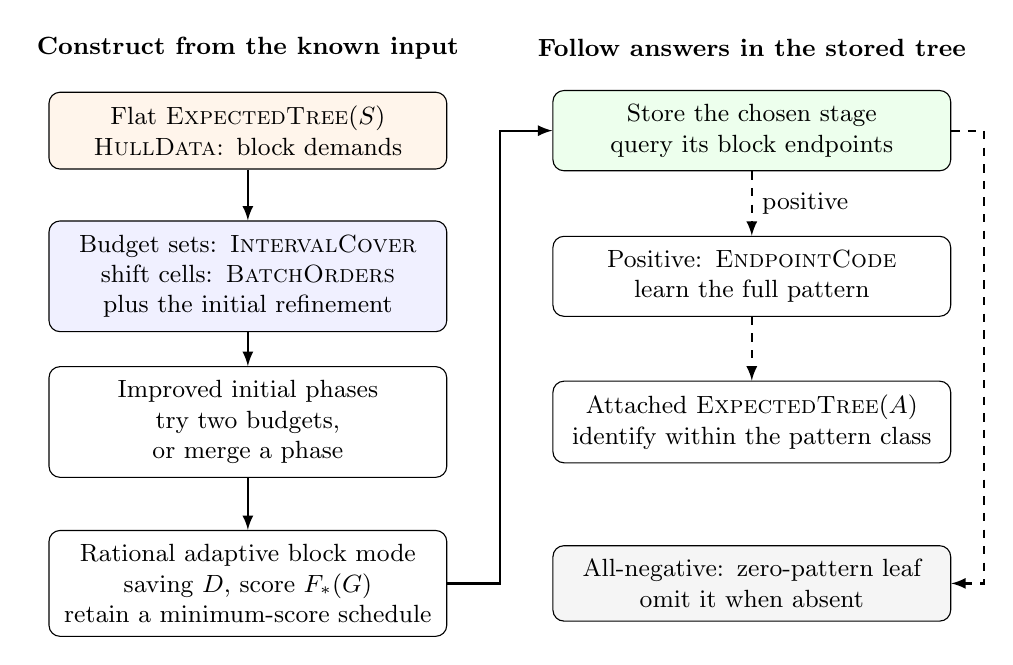
\begin{tikzpicture}[every node/.style={font=\small},
  box/.style={draw,rounded corners,align=center,inner sep=5pt,text width=4.7cm},
  arr/.style={-latex,thick},exec/.style={-latex,thick,dashed}]
  \node[font=\small\bfseries] at (-3.2,1.05) {Construct from the known input};
  \node[font=\small\bfseries] at (3.2,1.05) {Follow answers in the stored tree};
  \node[box,fill=orange!8] (hull) at (-3.2,0)
    {Flat \ExpectedTree$(S)$\\\HullData: block demands};
  \node[box,fill=blue!6] (covers) at (-3.2,-1.85)
    {Budget sets: \IntervalCover\\shift cells: \BatchOrders\\plus the initial refinement};
  \node[box] (variants) at (-3.2,-3.7)
    {Improved initial phases\\try two budgets, or merge a phase};
  \node[box] (score) at (-3.2,-5.75)
    {Rational adaptive block mode\\saving $D$, score $F_*(G)$\\retain a minimum-score schedule};
  \node[box,fill=green!7] (stored) at (3.2,0)
    {Store the chosen stage\\query its block endpoints};
  \node[box] (positive) at (3.2,-1.85)
    {Positive: \EndpointCode\\learn the full pattern};
  \node[box] (child) at (3.2,-3.7)
    {Attached \ExpectedTree$(A)$\\identify within the pattern class};
  \node[box,fill=gray!8] (zero) at (3.2,-5.75)
    {All-negative: zero-pattern leaf\\omit it when absent};
  \draw[arr] (hull) -- (covers);
  \draw[arr] (covers) -- (variants);
  \draw[arr] (variants) -- (score);
  \draw[arr] (score.east) -- (0,-5.75) -- (0,0) -- (stored.west);
  \draw[exec] (stored) -- node[right]{positive} (positive);
  \draw[exec] (positive) -- (child);
  \draw[exec] (stored.east) -- (6.15,0) -- (6.15,-5.75)
    -- (zero.east);
\end{tikzpicture}
\caption{The improved polynomial expected-depth procedure, including
the two-budget family of Algorithm~\ref{alg:two-phase-family}. The shift
cells include the refinement \eqref{eq:initial-shift-refinement}. Solid
arrows are construction-time data flow, computed from the supplied incidence
table and rational priors. Dashed arrows show how the unknown hypothesis
traverses the resulting tree; endpoint decoders and recursive children
are already constructed. Adaptive modes choose whether the first
positive block stops early or queries both endpoints. The certificate's
mixture is used in the proof of the bound, not to randomize execution.}
\label{fig:expected-procedure-flow}
\end{figure}



\subsection{One signed correction for each affected cost}

The unaveraged first-hit upper bound for the two-budget variant is
\[
 \begin{aligned}
 \phi_{u,q,r}(t)={}&\frac{q+1}{2}
  +\frac{q+r}{2}\mathbf1_{\{t>q\}}
  +\frac{r+k_2}{2}\mathbf1_{\{t>r\}}\\
 &+\frac12\sum_{j\ge2}(k_j+k_{j+1})\mathbf1_{\{t>k_j\}}.
 \end{aligned}
\]
For the one-budget variant, replace the two initial transition terms
by $(q+k_2)\mathbf1_{\{t>q\}}/2$.
Subtracting either bound from the old $\phi_u(t)$ gives the exact
doubled improvement
\begin{equation}\label{eq:two-phase-correction}
 \begin{aligned}
 d_{q,r}(u,t)={}&k_0-q+(k_0+k_1)\mathbf1_{\{t>k_0\}}
               +(k_1+k_2)\mathbf1_{\{t>k_1\}}\\
 &-(q+r)\mathbf1_{\{t>q\}}-(r+k_2)\mathbf1_{\{t>r\}},
       &&r>0,\\
 d_{q,0}(u,t)={}&k_0-q+(k_0+k_1)\mathbf1_{\{t>k_0\}}
               +(k_1+k_2)\mathbf1_{\{t>k_1\}}\\
 &-(q+k_2)\mathbf1_{\{t>q\}}.
 \end{aligned}
\end{equation}
The signs matter: changing a budget can delay some witness ranks.
Every modified budget sequence is strictly increasing, so its
first-hit upper bound is nondecreasing. An earlier actual comparison
hit therefore improves the bound. The within-batch proof of
Lemma~\ref{lem:mssc} applies to each sequence; early completion at
$Q_*$ only removes nonnegative residual terms.

The all-negative route has a different invoice. With $k=k_{\min}$,
its length change relative to the old unrolled budget sum is
\begin{equation}\label{eq:two-phase-zero-correction}
 z_{q,r}(u,k)=q\mathbf1_{\{q<k\}}+r\mathbf1_{\{r<k\}}
             -k_0\mathbf1_{\{k_0<k\}}
             -k_1\mathbf1_{\{k_1<k\}},
\end{equation}
where the $r$ term is zero for the one-budget variant.
This prices the complete negative route, rather than only the first
positive hit.

\subsection{A finite certificate and the common ledger}

Retain the witness masses $m_t$, prefix masses $M_q$, and discounts
$e_\beta(t)$ from Section~\ref{sec:polynomial-blocks}. Exact coverage
makes the first batch cover at least $M_q$ with at most $q$ blocks.
Its total adaptive-mode saving is therefore at least each of
\[
 \mathsf A_q=M_q-\delta wq,\qquad
 \mathsf C_q=c_*M_q-d_*\delta wq,\qquad 0,
\]
by Lemma~\ref{lem:affine-block-credit}. These remain valid if the first
batch completes the minimum cover. Later savings are nonnegative.

Section~\ref{sec:two-phase-certificate} gives a fixed rational
forty-three-row distribution of variants and first-batch minorants.
The shift is log-uniform, and each row has constant $k_0,k_1,k_2$.
For a row $[l,h)$ of probability $P=\ln(h/l)/\ln\beta$, an option
of conditional weight $v$ and minorant $sM_q-\rho\delta w$ contributes
\begin{equation}\label{eq:two-phase-coefficients}
 a_t\gets a_t+Pv\bigl[d_{q,r}(u,t)+s\mathbf1_{\{t\le q\}}\bigr],
 \qquad \mu\gets\mu+Pv\rho,
\end{equation}
starting with $a_t=e_\beta(t)$ and $\mu=0$.
This is a joint comparison of the actual schedule's signed first-hit
change and its actual saving:
\[
 \sum_t m_t e_\beta(t)+
 \mathbb E\left[\sum_t m_t d_{q,r}(u,t)
                     +\operatorname{Save}(G)\right]
 \ge\sum_t m_t a_t-\delta w\mu.
\]
No comparison rank is identified with an actual discovery rank, and
no saving is counted twice.

Take $\tau=2190079/10^6=2.190079$ and set
\begin{equation}\label{eq:two-phase-chi-B}
 \chi=\tau-2\delta(\tau-a_1)-\delta\mu,\qquad
 B=7-\frac{\ln6}{\ln\beta}-\chi.
\end{equation}
Exact outward logarithm enclosures give
\[
 \begin{aligned}
 1.276476788627&<a_1<1.276476788629<\tau,\\
 \min_{2\le t\le14}a_t&>2.1900797161>\tau,\\
 4.461183727318&<\mu<4.461183727321,\\
 1.199202587061&<\chi<1.199202587065,\\
 4.374727111309&<B<4.374727111314.
 \end{aligned}
\]
All saving cutoffs are at most six, $k_0\le3$, $k_1\le12$, and
$r\le13$. Hence every signed correction is constant for $t\ge14$.
For one constant $\kappa$, $a_t=e_\beta(t)+\kappa$ on that entire
tail; monotonicity of $e_\beta$ reduces it to the $a_{14}$ check.
Only $a_1$ lies below $\tau$.

Let $D_0(k)=\mathbb E[z_{q,r}(u,k)]$. The same certificate gives
$D_0(1)=0$ and, for $k=2,\ldots,14$ in that order,
\[
 \begin{split}
 D_0(k)<{}&-.24607,\ -.30801,\ -.33917,\ -.31328,
            \ -.26141,\ -.21949,\ -.18652,\\
          &-.15871,\ -.13510,\ -.11546,\ -.09779,
            \ -.08368,\ -.06992.
 \end{split}
\]
For $k\ge14$, $D_0(k)=D_0(14)$, since all affected budgets are at
most thirteen. Thus the full mean waiting length still satisfies
$\mathbb E[|G|]\le Z_\beta(k_{\min})$ for every cover size. The
supporting witness and $\lambda_\beta>\nu_\beta$ retain the original
zero-route credit $2p_0/\ln\beta$.

Finally, the certificate gives $\chi+2/\ln\beta>\tau$.
Lemma~\ref{lem:capped-rank-credit} applies with $E=\{1\}$ and
$\zeta=2/\ln\beta$, converting all these terms into the saving
$\chi b$. Choosing the minimum rational score costs at most averaging
that score over the fixed distribution. Substitution into
\eqref{eq:adaptive-stage} yields the same local ledger as before:
\begin{equation}\label{eq:two-phase-local}
 W_{\rm pat}(S)\le A\Delta+B b+\frac{I-J_*}{\ln2},
 \qquad A=\frac{\beta+1}{\ln\beta}.
\end{equation}
The degenerate hull also satisfies this bound because $A,B>2$.

\begin{theorem}[Two-initial-budget polynomial approximation]
\label{thm:two-phase-expected}
For general supplied binary unit-cost planar line queries and arbitrary
strictly positive rational priors, the two-initial-budget adaptive
algorithm runs in deterministic polynomial time and has factor
\[
 \boxed{\rho_{\rm two}=
 A+\max\{\ln2/h(\delta),\ B\ln2/\sigma(\delta)\}<5.182976.}
\]
Its running-time exponent has no dependence on the smallest prior.
\end{theorem}
\begin{proof}
Apply Lemma~\ref{lem:stage-conversion} to
\eqref{eq:two-phase-local} and \eqref{eq:coarse-discovery-cap}.
Here $6<1/\delta<7$, so
$\sigma(\delta)=-6\delta\ln\delta
 -(1-6\delta)\ln(1-6\delta)$.
The rational logarithm bounds \eqref{eq:rational-log-bounds} certify
all comparisons above and
\[
 A+\max\{\ln2/h(\delta),B\ln2/\sigma(\delta)\}
 <5.182975508794<5.182976.
\]
The reproducible certificate \texttt{expected-two-phase-check.py}
also verifies $\lambda_\beta>\nu_\beta$, the accepted entropy tent,
$9{,}900$ exact signed-phase identities, and $1{,}650$ finite modified
batch comparisons including early completion and negative-route
lengths. The proof uses the fixed rational data of
Section~\ref{sec:two-phase-certificate}; it has no floating-point
optimization assumption.

The family adds a constant number of candidates per polynomial shift
partition. Coverage DPs, mode scores, and all decisions remain
rational and polynomial; the full-pattern recursive classes remain
disjoint proper subsets. Every actual query is a supplied endpoint
line. The singleton and degenerate-hull procedures retain their
existing guarantees.
\end{proof}

\section{Quasipolynomial improvements}
\label{sec:quasipolynomial}

The construction has two steps. First, a dynamic program chooses one
block order satisfying a logarithmic number of nested deadlines, or
minimizing the corresponding weighted delay. Combined with the
supporting-prefix and endpoint lemmas, this gives a legal baseline tree
with cost $2\lambda\OPT$ plus a logarithmic or entropy penalty, where
$\lambda>1$ is the grade spacing. Second, exact optimization of a
logarithmic-depth initial tree removes that penalty. Together these
steps give $(2+\varepsilon)$ approximations for both objectives.
Every query remains a supplied line. Optimal witness paths occur only
in the analysis: the algorithms use interval demands, actual child
costs, and the supplied prior.

\subsection{Nested interval deadlines}

Algorithm~\ref{alg:grade-dp} gives the shared DP; Algorithm~\ref{alg:qp-baselines}
uses it in the two recursions, and Algorithm~\ref{alg:rollout} performs
the exact initial-tree optimization.

Let $M$ candidates be in linear spatial order, and suppose interval
demands have deadlines among $b_1<\cdots<b_r$. A selected candidate is
assigned a grade $i\in[r]$. Scan positions from left to right and store
for each grade prefix $j$ its selected count $c_j$ and last selected
position $p_j$ (zero if none). Selecting position $q$ at grade $i$
increments $c_j$ and sets $p_j=q$ for every $j\ge i$; skip is the
other transition. Reject if $c_j>b_j$. When $[l,q]$ of deadline
$b_j$ ends, require $p_j\ge l$. The invariant is that these are
exactly the count and rightmost selected position among scanned
candidates of grade at most $j$. Thus the interval check is equivalent
to having a qualifying selected point in that demand.

Listing selected candidates in grade order yields a schedule: each
deadline-$b_j$ demand is met in its grade prefix, whose length
$c_j\le b_j$. Conversely, give each query in any feasible schedule
the first deadline bucket at least its rank and discard queries after
all deadlines. This maps every feasible schedule to a DP witness, so
the test is exact. There are at most $(M+1)^r(B+1)^r$ states for
$B=\max b_j$, with $r+1$ transitions per position. For circular
demands, enumerate the first candidate $v$, remove demands containing
it, and cut there. Its forced rank-one query consumes one unit in
\emph{every} cumulative count, so residual capacities are $b_j-1$.

Independent coverage at each deadline need not be jointly feasible.
On candidates $1,2,3$, let $[1,2]$ and $[2,3]$ have deadline one,
and let $\{1\}$ and $\{3\}$ have deadline two. Each prefix is
separately coverable, but no ordering works: 2 must be first, and then
both 1 and 3 are needed by rank two. The grade-vector DP captures this
nesting constraint.

\begin{algorithm}[H]
\caption{\GradeDP: cumulative-grade interval feasibility or weighted delay}
\label{alg:grade-dp}
\KwIn{Ordinary intervals; capacities $b_0<\cdots<b_r$;
feasibility deadlines, or weights and delay levels $d_j=b_j-1$.}
\KwOut{A feasible graded selection, or a minimum surrogate-delay selection.}
Initialize the state $(c_0,\ldots,c_r;s_0,\ldots,s_r)$ to all zeros,
with cost zero; all other states are unreachable\;
\For{$q=1,\ldots,M$}{
  From each reachable state, try skipping $q$ or selecting it at grade $i$\;
  A grade-$i$ selection increments $c_j$ and sets $s_j=q$ for all $j\ge i$\;
  Reject any transition with $c_j>b_j$\;
  \ForEach{interval $I=[l,q]$ ending here}{
    \eIf{mode is feasibility}{
      Reject if $s_j<l$ for its deadline grade $j$\;
    }{
      Find the least $j$ with $s_j\ge l$; reject if none\;
      Add $2w(I)d_j$ to this transition's cost\;
    }
  }
  Keep one feasible witness, or the minimum cost, for each resulting state\;
}
In weighted mode add $2p_0c_r$ to each final state's cost\;
Reconstruct a winning selection and order it by grade\;
\KwRet the selection and schedule, or infeasible\;
\end{algorithm}

For circular demands enumerate the forced first candidate, remove
its demands, cut there, and reduce \emph{every} capacity by one.
Residual expected costs still use the original delay levels and add
$2p_0(1+c_r)$ at completion. In maximum-depth mode append a final
grade with the total-count cap if it is not already a capacity.
Section~\ref{sec:quasipolynomial} proves the state invariant and
the $(M+1)^{O(r)}(B+1)^{O(r)}$ bound.


\subsection{Adjacent support blocks and shifted delays}

Use the edges of the full normalized hull, including the origin if
it is a hull vertex, as candidate \emph{blocks}. Within a block,
query its real endpoints in a fixed order, skipping cached answers;
the origin is a free known-negative marker and is never queried.
A positive vertex interval meets a consecutive circular interval of
edges, obtained by including its incident edges. Thus the block-hit
demands are circular intervals too. A two-support original query
maps to its supporting edge; a singleton support maps to any incident
edge. This can only make a class get hit earlier. Repeated or
unproductive blocks may be deleted. In dimension at most one, the
at most two real vertices determine the pattern directly, and the
same upper bounds apply.

Write $k$ for the first hitting block's rank and
$z_A=\lfloor\log_2(\delta s/|A|)\rfloor$ in a count-flat state.
If the first queried endpoint is positive, discovery and endpoint
recovery cost at most $2k-1+z_A+4$.
If the second endpoint is the first positive answer, its adjacent
endpoint is known negative, so the cost is at most $2k+z_A+2$.
A block with just one real endpoint costs at most $2k-1+z_A+4$.
Consequently all routes obey
\begin{equation}\label{eq:qp-block-allowance}
 \text{discovery plus endpoint cost for }A\ \le 2(k-1)+z_A+5.
\end{equation}
For expected depth the same accounting gives an overhead of at most
five per unit of nonzero-pattern mass, in addition to the residual
pattern entropy. Pairing the queries preserves the saving from the
negative first endpoint on a second-endpoint exit.

\begin{algorithm}[H]
\caption{Graded adjacent-block recursion: the quasipolynomial baselines}
\label{alg:qp-baselines}
\KwIn{State $S$; objective $o$; rational $\lambda>1$ and the associated balance parameters.}
\KwOut{The baseline tree of Section~\ref{sec:quasipolynomial}.}
Stop at a singleton; at a balanced state query a balanced line and recurse\;
At a flat state compute $\HullData(S)$ and use full-hull edges as blocks\;
Handle a hull of dimension at most one by its direct extreme tests\;
\eIf{$o=\mathrm W$}{
  Build the pattern children once and record their heights $C_W(A)$\;
  \For{trial heights $H$ in increasing order}{
    Compute $B_A=\lfloor(H-C_W(A)-z_A-5)/2\rfloor$; reject negative budgets\;
    Round each down to the last level in $\{0\}\cup\{\lfloor\lambda^j\rfloor\}$ not exceeding it\;
    Use deadlines $\widehat B_A+1$ and total cap $\lfloor H/2\rfloor$
    in circular $\GradeDP$; stop at the first feasible trial\;
  }
}{
  Use distinct levels $d_0=0$, $d_j=\lfloor\lambda^j\rfloor$ through a level covering $n$\;
  Minimize the circular weighted-delay surrogate with capacities $d_j+1$
  by $\GradeDP$ and zero-pattern mass $w(A_0)$\;
}
Execute the selected blocks, use pointwise endpoint codes for $\mathrm W$
or expected endpoint codes for $\mathrm E$, and attach recursive pattern children\;
Identify the zero singleton after the negative cover if present; omit it otherwise\;
\KwRet the contracted tree\;
\end{algorithm}

The maximum-depth trial range is
$1\le H\le\lceil(2\lambda+\gamma)(|S|-1)\rceil$.
No optimum value or comparison witness is an algorithm input.


\subsection{Maximum depth}

Fix rational $\lambda>1$, $a=2\lambda$, and rational
$0<\delta<1/3$, $\gamma\ge1$ satisfying
\begin{equation}\label{eq:qp-max-parameters}
 \gamma\log_2\frac1{1-\delta}\ge1,\qquad
 \gamma\log_2\frac1\delta\ge5.
\end{equation}
The algorithm constructs a tree satisfying
\begin{equation}\label{eq:qp-max-induction}
 C_W(S)\le\left\lfloor a\OPT_W(S)+\gamma\log_2|S|\right\rfloor.
\end{equation}
At a flat state, first construct all pattern-child codes and record
their actual heights $C_W(A)$. Enumerate a trial height $H$ and a
forced first block. For each nonzero class set the integer delay budget
\[
 B_A=\left\lfloor\frac{H-C_W(A)-z_A-5}{2}\right\rfloor.
\]
Reject negative budgets. Round each $B_A$ down to the largest level
$\widehat B_A$ in $\{0\}\cup\{\lfloor\lambda^j\rfloor:j\ge0\}$
not exceeding it, and give the class the block-rank deadline
$\widehat B_A+1$. Demands hit by the first block are removed; its
rank consumes one unit of every prefix capacity, so remaining
capacities are $\widehat B_A$. Cut the circular block order there
and use the nested interval-deadline DP. Also cap the total selected
block count, including the forced block, at $\lfloor H/2\rfloor$.
Order the selected blocks by grade, execute them, and attach the
endpoint exits and child codes. The all-negative route stops after
all nonzero patterns are covered and identifies the zero singleton,
if present. Trials need only reach
$\lceil(a+\gamma)(|S|-1)\rceil$.

To prove the induction, put $s=|S|$, $D=\OPT_W(S)$,
$x=\log_2(s/|A|)$, $L=\log_2(1/\delta)$, and let $t=t_A$ be the
supporting-prefix index. Restriction gives
$\OPT_W(A)\le D-(t-1)$. At
$H^*=\lfloor aD+\gamma\log_2s\rfloor$, the integer
$E_A=H^*-C_W(A)-z_A-5$ satisfies
\begin{align*}
 E_A&\ge\lfloor a(t-1)+\gamma x\rfloor-\lfloor x-L\rfloor-5\\
 &\ge\lfloor a(t-1)+(\gamma-1)x+L\rfloor-5\\
 &\ge\lfloor a(t-1)+\gamma L\rfloor-5
 \ge\lfloor a(t-1)\rfloor.
\end{align*}
Here $x>L$, $\gamma\ge1$, and \eqref{eq:qp-max-parameters} were
used. It follows that
\[
 B_A\ge\left\lfloor\frac{\lfloor2\lambda(t-1)\rfloor}{2}\right\rfloor
 =\lfloor\lambda(t-1)\rfloor.
\]
For $t=1$ the zero delay level suffices. Otherwise, if
$\widehat B_A=\lfloor\lambda^j\rfloor$, choose $j$ as the last
exponent with $\lfloor\lambda^j\rfloor\le B_A$, including any
duplicate-floor plateau. Maximality then gives
$\lambda^{j+1}\ge B_A+1>\lambda(t-1)$, hence
$\widehat B_A\ge t-1$. This downward rounding retains the exact
integer credit; rounding a real expression first would not suffice.

Map the optimal witness path into its supporting blocks. Every
class is hit by block rank at most $t_A$, and therefore meets its
deadline. If the path terminates at an uncovered nonzero singleton,
append an incident block hitting it; its supporting-prefix index
is $q+1$. The block count is at most $D$ when the zero pattern is
present and at most $D+1$ otherwise. The constraints imply
$\gamma>2$: for $\delta\le1/4$ the first parameter inequality
gives $\gamma\ge1/\log_2(4/3)>2$, while for $\delta>1/4$
the second gives $\gamma>5/2$. Hence for $s\ge2$,
$\lfloor H^*/2\rfloor\ge D+1$. Thus the comparison fits the total
count cap. Enumerating its first block proves trial $H^*$ feasible.
Equation~\eqref{eq:qp-block-allowance} then bounds every positive
exit by $H^*$; the zero route costs at most $H^*$ as well.
Balanced states use the same one-query count-potential argument,
completing the induction.

Since $D\ge\log_2s$, the direct factor is at most $a+\gamma$.
Use the manuscript's rational maximum-depth parameters
$\delta=245122334/10^9$ and $\gamma=246496526/10^8$.
For $\lambda=10000001/10000000$ this gives
\[
 a+\gamma=4.46496546<4.464966.
\]
The less fine grading $\lambda=2001/2000$ gives a factor below $4.466$.
The limiting bound is approximately $4.46496526$, at the solution of
$\delta=(1-\delta)^5$. The rational inequalities are certified by
the logarithm series in \eqref{eq:rational-log-bounds}.
There are $O(\log n/(\lambda-1))$ grades, with polynomially bounded
counts and last positions. The state space and total running time
are $(mn)^{O(\log n/(\lambda-1))}$ for fixed parameters, with
rational arithmetic of polynomial bit length.

\subsection{Arbitrary-prior expected depth}

For positive block demands $I$ of weights $w(I)$ and zero-pattern
mass $p_0\ge0$, minimize over block orders $Q$
\[
 F(Q)=2\sum_I w(I)(\operatorname{first}_Q(I)-1)+2p_0|Q|.
\]
An optimum uses at most the number of demands, since unproductive
blocks can be deleted. Use delay level $d_0=0$ and distinct positive
levels $d_j=\lfloor\lambda^j\rfloor$ through a level covering $n$.
The spatial DP stores grade-prefix last positions $p_j$ and counts
$c_j\le d_j+1$. When interval $[l,q]$ ends,
let $\tau(I)$ be the least $j$ with $p_j\ge l$; reject if none exists
and charge $2w(I)d_{\tau(I)}$. Keep the least accumulated cost per
state and add $2p_0c_{\rm last}$ at completion. Each interval is
charged once at its right endpoint, and $\tau(I)$ is its earliest
selected grade. Ordering selected blocks by grade gives actual hit
delay at most $d_{\tau(I)}$ and length exactly $c_{\rm last}$.

Rank $k=1$ has delay zero and uses grade zero. For $k\ge2$, the
first positive level at least $k-1$ satisfies $d_j<\lambda(k-1)$.
Assigning comparison-order
blocks to these grades respects every capacity $d_j+1$. Thus the
minimum surrogate is at most $\lambda$ times the positive delay
cost plus the unchanged zero waiting cost, and hence at most
$\lambda F(Q)$ for any comparison $Q$. For circular demands
enumerate the first block, remove demands containing it at charge
zero, and cut there. Reduce every cumulative capacity by one and add
$2p_0(1+c_{\rm last})$. Enumerating the comparison's first block
and assigning its remaining blocks by their absolute ranks proves
the same guarantee.
This exact optimization DP has quasipolynomial
$(mn)^{O(\log n/(\lambda-1))}$ running time and polynomial-bit rational
arithmetic.

To bound the comparison ordering, let
$D_+=\sum_{A\ne A_0}w(A)(t_A-1)$ and
$b=\sum_{A\ne A_0}w(A)$. The supporting-block witness order hits
each class by block rank $t_A$. An uncovered terminal nonzero
singleton can be hit by appending an incident block. If $A_0$
exists, the number of blocks is at most the witness path length $q$;
the supporting-prefix lemma gives
$D_++w(A_0)q\le\Delta_{\mathrm E}(S,\Pi)$. The cover-order guarantee
therefore bounds the selected schedule's delay and zero waiting
cost by $2\lambda\Delta_{\mathrm E}$. If $A_0$ is absent, the
appended singleton is covered by its index $t=q+1$ and there is
no zero waiting term.

Write $I=I(S,\Pi)$ for full-pattern information and $J$ for the
discovery-transcript information. The first-endpoint exits have
discovery cost at most $2(k-1)+1$ and endpoint overhead four;
second-endpoint exits have discovery cost at most $2(k-1)+2$ and
overhead two because their neighbor is known negative. Thus
\[
 W_{\rm stage}\le2\lambda\Delta_{\mathrm E}
 +5b+(I-J)/\ln2.
\]
The actual vertex-answer transcript is used for $J$, so every
nonzero discovery cell still lies in one cap of mass below $\delta$,
even though a block can meet the union of two caps.
In a flat state, the capped-discovery lemma gives $J\ge b\sigma(\delta)$,
where
\[
 h(\delta)=-\delta\ln\delta-(1-\delta)\ln(1-\delta),\quad
 k=\lfloor1/\delta\rfloor,\quad r=1-k\delta,\quad
 \sigma(\delta)=-k\delta\ln\delta-r\ln r,
\]
and $0\ln0=0$. Put
\[
 c=\max\{1/h(\delta),\ 5/\sigma(\delta),\ 1/\ln2\}.
\]
Apply Lemma~\ref{lem:stage-conversion} with $A=2\lambda$ and
$B=5$. It pays for endpoint overhead from the discovery information,
then telescopes the remaining restriction and entropy terms. Thus
\begin{equation}\label{eq:qp-expected-ratio}
 C_{\mathrm E}(S)\le2\lambda\OPT_{\mathrm E}(S)+c\mathcal E(S),\qquad
 R\le2\lambda+\max\left\{\frac{\ln2}{h(\delta)},
 \frac{5\ln2}{\sigma(\delta)},1\right\}.
\end{equation}
There is no subtraction of one from the endpoint coefficient because
the remaining pattern entropy still has to be paid.

Take $\lambda=100001/100000$ and $\delta=139087/10^6$. For an exact
certificate use the rational logarithm bounds to verify
\[
 (42967/25000)h(\delta)>\ln2,\qquad
 (42967/25000)\sigma(\delta)>5\ln2.
\]
Thus both terms in the maximum are below $42967/25000=1.71868$, and
\begin{equation}\label{thm:qp-expected}
 C_{\mathrm E}(S)<\frac{37187}{10000}\OPT_{\mathrm E}(S)
 =3.7187\OPT_{\mathrm E}(S).
\end{equation}
As $\lambda\to1$, numerical optimization of this bound approaches
$3.71867512$ near $\delta=0.13908730$; the limit is numerical,
whereas $3.7187$ is the certified bound. The guarantee applies to
arbitrary strictly positive priors and is independent of the smallest
probability.

\subsection{Logarithmic-depth lookahead: factors approaching two}

Algorithm~\ref{alg:rollout} optimizes the first $k$ levels and then
attaches a baseline tree at each surviving state. Its guarantee uses
the same principle for both objectives: each level already paid for
at unit cost replaces a level charged at factor $a>1$ in the baseline.
For maximum depth this saving is pathwise; for expected depth it is
weighted by the mass still on the frontier.

Let $B_W(S)$ and $B_E(S)$ be the actual baseline costs, zero on
singletons. Set $F_0(S)=B_W(S)$ and $G_0(S)=B_E(S)$. For $j\ge1$,
the exact initial-tree recurrences are
\begin{align*}
 F_j(S)&=\min\left\{B_W(S),\;
 1+\min_{\ell\text{ splits }S}\max_{b\in\{0,1\}}F_{j-1}(S_{\ell,b})
 \right\},\\
 G_j(S)&=\min\left\{B_E(S),\;
 w(S)+\min_{\ell\text{ splits }S}
 \bigl(G_{j-1}(S_{\ell,0})+G_{j-1}(S_{\ell,1})\bigr)\right\}.
\end{align*}
The baseline option permits earlier stopping. Queries constant on
$S$ are omitted, and expected costs retain the original prior
weights. Memoizing $(S,j)$ and retaining minimizing choices gives
a legal tree attaining these values. The comparison tree in the
next lemma establishes an upper bound; it is never an input to the
recurrences.

\begin{lemma}[Lookahead removes bounded continuation penalties]
\label{lem:lookahead-completion}
Fix $a>1$ and integer $k\ge0$. Suppose that, on every restricted
state $S'$, a legal baseline obeys one of the following bounds:
\[
 B_W(S')\le a\OPT_W(S')+L_W,
 \qquad\text{or}\qquad
 B_E(S')\le a\OPT_E(S')+L_Ew(S').
\]
The exact $k$-level lookahead with that baseline is an
$a$-approximation if $k\ge L_W/(a-1)$ or, respectively,
$k\ge L_E/(a-1)$. Baseline costs at singletons are zero.
\end{lemma}
\begin{proof}
For maximum depth, truncate an optimal height-$D$ tree at depth
$k$. A leaf reached earlier has depth at most $D$. If $D<k$,
the whole optimal tree is a candidate. Otherwise each surviving
frontier state $S'$ satisfies $\OPT_W(S')\le D-k$, so its completed
branch has height at most
\[
 k+a(D-k)+L_W=aD-(a-1)k+L_W\le aD.
\]

For expected depth, truncate an optimal tree $T^*$ at depth $k$.
Let $P$ be its expected prefix cost and $R$ the sum of its continuation
costs. Optimality of the continuations gives
$P+R=\OPT_E(S)$. The surviving frontier states are disjoint; write
$M_k$ for their total mass. Every hypothesis in those states has
already paid for $k$ queries, so $P\ge kM_k$. Completing them with
the baseline therefore costs at most
\begin{align*}
 P+aR+L_EM_k
 & =a\OPT_E(S)-(a-1)P+L_EM_k\\
 &\le a\OPT_E(S)+\bigl(L_E-(a-1)k\bigr)M_k
 \le a\OPT_E(S).
\end{align*}
This argument uses expected prefix cost directly and makes no
assumption on $T^*$'s maximum depth or on the smallest prior mass.
Exact lookahead can only improve on either completed comparison tree.
\end{proof}

\begin{algorithm}[H]
\caption{\Rollout: exact initial-tree optimization with a baseline}
\label{alg:rollout}
\KwIn{State $S$, objective $o$, lookahead $j$, and legal baseline routine $B$.}
\KwOut{The cheapest initial tree of at most $j$ levels, completed by $B$.}
\If{$|S|\le1$}{\KwRet its leaf\;}
\If{$(S,o,j)$ is memoized}{\KwRet the stored tree and cost\;}
Compute the actual baseline tree $B(S)$ and retain it as the initial best choice\;
\If{$j>0$}{
  \ForEach{supplied line $\ell$ splitting $S$}{
    Recurse on $S_\ell^-,S_\ell^+$ with lookahead $j-1$\;
    Compare $1+\max\{v_-,v_+\}$ if $o=\mathrm W$,
    or $w(S)+v_-+v_+$ if $o=\mathrm E$, with the best cost\;
    Store a lower-cost choice and its two child trees\;
  }
}
Memoize and return the best choice\;
\end{algorithm}

For Theorem~\ref{thm:qp-two-plus-epsilon}, use Algorithm~\ref{alg:qp-baselines}
with $\lambda=1+\varepsilon/2$ and a lookahead at least
$\gamma\log_2 n/(2\lambda-1)$ for maximum depth or
$c\ln n/(2\lambda-1)$ for expected depth. Rational upper bounds and
$\lceil\log_2 n\rceil$ give implementable integer caps; cap at $n-1$.


\begin{figure}[htbp]
\centering
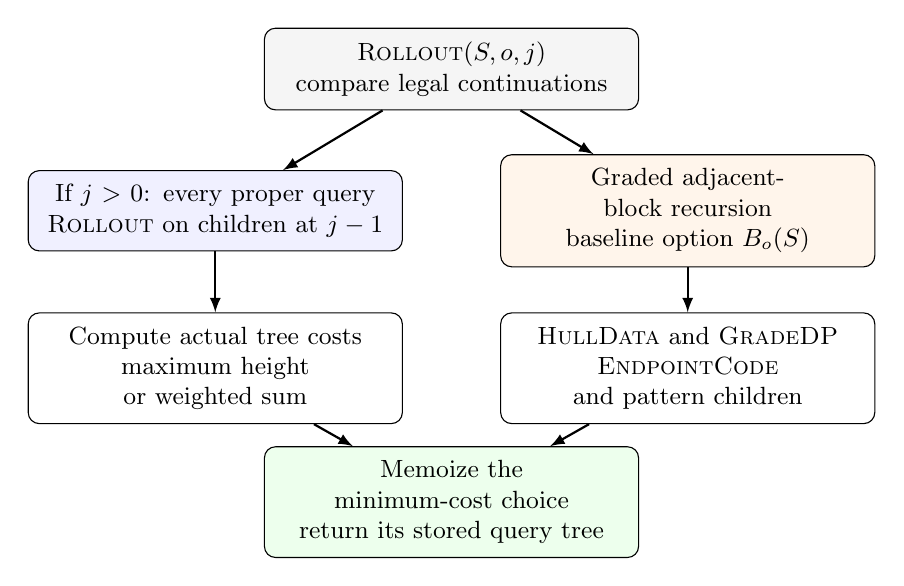
\begin{tikzpicture}[every node/.style={font=\small},
  box/.style={draw,rounded corners,align=center,inner sep=5pt,text width=4.4cm},
  arr/.style={-latex,thick}]
  \node[box,fill=gray!8] (rollout) at (0,0)
    {\Rollout$(S,o,j)$\\compare legal continuations};
  \node[box,fill=blue!6] (split) at (-3,-1.8)
    {If $j>0$: every proper query\\\Rollout\ on children at $j-1$};
  \node[box,fill=orange!8] (baseline) at (3,-1.8)
    {Graded adjacent-block recursion\\baseline option $B_o(S)$};
  \node[box] (grade) at (3,-3.8)
    {\HullData\ and \GradeDP\\\EndpointCode\ and pattern children};
  \node[box] (evaluate) at (-3,-3.8)
    {Compute actual tree costs\\maximum height or weighted sum};
  \node[box,fill=green!7] (best) at (0,-5.5)
    {Memoize the minimum-cost choice\\return its stored query tree};
  \draw[arr] (rollout) -- (split);
  \draw[arr] (rollout) -- (baseline);
  \draw[arr] (baseline) -- (grade);
  \draw[arr] (split) -- (evaluate);
  \draw[arr] (grade) -- (best);
  \draw[arr] (evaluate) -- (best);
\end{tikzpicture}
\caption{Exact lookahead wrapped around the quasipolynomial baseline.
The arrows denote calls and the returned trees or costs. The baseline
may end lookahead early at any reached state. The logarithmic cap on
$j$ bounds the number of reachable transcripts; it does not truncate
the completed identification tree. The proof compares this finite
search with an optimal tree, but the search evaluates only constructed
trees.}
\label{fig:qp-procedure-flow}
\end{figure}


\begin{theorem}\label{thm:qp-two-plus-epsilon}
For every fixed rational $\varepsilon>0$, both maximum depth and
arbitrary-prior expected depth admit quasipolynomial-time
$(2+\varepsilon)$ approximations using only supplied binary line
queries. For $0<\varepsilon\le1$, the running time is
$(mn)^{O(\varepsilon^{-1}\log n)}$ times a polynomial in the input
bit length. This scheme approaches factor two.
\end{theorem}
\begin{proof}
For $0<\varepsilon\le1$, take $\lambda=1+\varepsilon/2$ and
$a=2\lambda=2+\varepsilon$ in the two baseline constructions.
Their additive bounds imply the hypotheses of
Lemma~\ref{lem:lookahead-completion} with
\[
 L_W=\gamma\log_2n,\qquad L_E=c\ln n,
\]
because $\log_2|S'|\le\log_2n$ and
$\mathcal E(S')\le w(S')\ln n$. Choose the corresponding lookahead
length from that lemma. For $\varepsilon>1$, run the construction
with $\varepsilon=1$.

For implementation, choose fixed rational upper bounds on $\gamma$
and $c$, and replace logarithms in the lookahead lengths by
$\lceil\log_2 n\rceil$, which also upper-bounds $\ln n$.
Cap $k$ at $n-1$ if necessary; that permits every proper tree and
returns the exact optimum. The lookahead depth is $O(\log n)$
because $a-1\ge1$. At most $(2m)^{O(k)}$ states are reachable,
since each is determined by at most $k$ supplied query answers.
Each baseline call has $(mn)^{O(\varepsilon^{-1}\log n)}$ cost:
there are $O(\varepsilon^{-1}\log n)$ schedule grades, and their
counts and last positions have polynomial ranges. Multiplying the
two bounds gives the stated running time. Powers of rational
$\lambda$, count
capacities, and original prior weights have polynomial bit length
for fixed $\varepsilon$; the optimized objectives are rational
sums of actual tree costs. Thus no irrational comparisons are
required in the dynamic programs.
Every retained query properly splits its state, so the reconstructed
tree has at most $n$ leaves and $n-1$ internal nodes.
\end{proof}

\section{Polynomial maximum depth with rank-subset scheduling}
\label{sec:polynomial-slots}

The direct maximum-depth guarantee in
Section~\ref{sec:quasipolynomial} can be obtained in polynomial time.
The key is an exact interval-deadline algorithm exponential in the
\emph{total number of schedule slots}, rather than in the number of
distinct deadline grades. Restrict this algorithm to a logarithmic
number of slots and retain the priority schedule as a fallback.
Two simultaneous recursive bounds then cover all instances.
The algorithm checks schedules against the heights of its own stored
children. An optimal witness path is used only to prove that a passing
schedule exists; neither that path nor its optimum height is an input.

\subsection{Exact interval deadlines with a bounded number of ranks}

Algorithm~\ref{alg:slot-dp} specifies the rank-subset DP, and
Algorithm~\ref{alg:hybrid-tree} gives the capped recursion.
Candidates are the integers $1,\ldots,M$. A demand is an interval
$[a,b]$ with an integer deadline $d_{[a,b]}$: some selected candidate
in that interval must occur by rank $d_{[a,b]}$. Selected candidates
are distinct, and the total schedule length is at most $L$.

\begin{lemma}[Rank-subset interval scheduling]
\label{lem:rank-subset-scheduling}
Interval-deadline feasibility and a feasible schedule can be computed
in $O(M^3 3^L+NM^2)$ time with $O(M^2 2^L)$ dynamic-programming
states, where $N$ is the number of demands. For circular intervals,
enumerating the first candidate adds a factor $M$.
\end{lemma}
\begin{proof}
For a spatial region $[l,r]$, let $\mathcal I(l,r)$ contain precisely
the original demands wholly inside that region. These are exactly
the demands still unhit: a demand crossing an earlier separator was
hit there, whereas a contained demand contains no earlier separator.
A state
$F(l,r,T)$, with $T\subseteq\{1,\ldots,L\}$, asks whether those
demands can be hit using candidates in $[l,r]$ assigned distinct
absolute ranks from $T$. Ranks may remain unused.
Keeping their absolute values allows queries in the left and right
regions to be interleaved without losing either region's deadlines.

If $\mathcal I(l,r)$ is empty, the state is true. If it is nonempty
and $T$ is empty, the state is false. Otherwise put $t=\min T$;
reject if any contained demand has deadline less than $t$. Enumerate
a candidate $p\in[l,r]$ and a partition
$T\setminus\{t\}=T_L\mathbin{\dot\cup}T_R$. Accept if
\[
 F(l,p-1,T_L)\quad\hbox{and}\quad F(p+1,r,T_R)
\]
both accept. Candidate $p$ is queried at rank $t$. All demands
containing it are now hit; every remaining demand is wholly inside
exactly one child region.

The earliest available rank can always be used: move the first query
of any feasible state to $\min T$, which only accelerates hits.
The resulting recursion is the spatial Cartesian tree of a schedule,
whose root is its earliest query. Its left and right descendants
partition the remaining assigned ranks, giving a successful transition.
Conversely, a successful recurrence
assigns distinct ranks meeting every deadline. Reconstruction sorts
the selected points by rank and deletes unused slots, again only
accelerating hits.

The existence and minimum deadline of contained demands can be
precomputed in $O(NM^2)$ time. There are $O(M^2 2^L)$ states, and
the total number of rank partitions over all masks is bounded by
$\sum_T2^{|T|}=3^L$. Trying $M$ root candidates gives the stated time.
For a circular instance, enumerate its first selected candidate,
discard the demands it hits, and cut the circle there. All surviving
demands are ordinary intervals. Subtract one from their deadlines and
use $L-1$ slots. A surviving demand with deadline at most one rejects
that trial. Enumerating the first candidate is exact.
\end{proof}

\begin{algorithm}[H]
\caption{\SlotDP: exact interval deadlines with a rank subset}
\label{alg:slot-dp}
\KwIn{Ordinary interval demands and deadlines; region $[l,r]$;
available absolute ranks $T\subseteq[L]$.}
\KwOut{A feasible rank assignment, or infeasible.}
\If{no original demand is wholly contained in $[l,r]$}{\KwRet the empty assignment\;}
\If{$T=\varnothing$}{\KwRet infeasible\;}
\If{this state is memoized}{\KwRet its stored result\;}
$t\gets\min T$\;
\If{a wholly contained demand has deadline $<t$}{\KwRet infeasible\;}
\ForEach{$p\in[l,r]$ and $T_L\subseteq T\setminus\{t\}$}{
  $T_R\gets T\setminus(T_L\cup\{t\})$\;
  Recurse on $([l,p-1],T_L)$ and $([p+1,r],T_R)$\;
  \If{both assignments are feasible}{
    Memoize their union with $(p,t)$ and \KwRet it\;
  }
}
Memoize and return infeasible\;
\end{algorithm}

Sort selected candidates by their ranks and suppress unused ranks.
The circular wrapper forces the first candidate, cuts there, and
subtracts one from surviving deadlines and the slot cap.
For the optional complete-exit variant, precompute the two oriented
decoder costs by Algorithm~\ref{alg:endpoint-code}; replace the deadline
precheck by the two local height tests of
Section~\ref{sec:polynomial-slots}. The same rank partitions apply.


\subsection{The hybrid recursive algorithm}

Use the rational count parameters of Section~\ref{sec:worst},
\[
 \delta=\frac{245122334}{10^9},\qquad
 \gamma=\frac{246496526}{10^8}.
\]
Let $n$ be the size of the \emph{original} instance and fix
\begin{equation}\label{eq:global-slot-cap}
 q=\lceil\log_2n\rceil,\qquad
 R=\left\lfloor\frac{\gamma q}{\gamma-1}\right\rfloor,
 \qquad L=R+1.
\end{equation}
This cap is retained throughout the recursion; it is not recomputed
from a child's size. Singleton states stop, and count-balanced states
use the existing balanced-query rule.

At a count-flat state $S$, build each full hull-pattern child's
\emph{hybrid} code once and record its actual height $C_W(A)$.
For each trial height $H$, consider both the existing priority
construction and a capped exact adjacent-block construction. Choose
the least passing trial over the two alternatives. Both use the same
already-built child codes.
The priority alternative guarantees that some trial passes. The exact
alternative can improve that trial when a short comparison schedule
exists; the algorithm tries it without testing the unknown optimum.

For the exact alternative, candidate blocks are edges of the full
normalized hull, retaining the origin as a free negative marker when
it is a hull vertex. Every nonzero pattern induces a circular interval
of blocks that meet its positive vertex arc. Put $s=|S|$ and
\[
 z_A=\lfloor\log_2(\delta s/|A|)\rfloor,\qquad
 B_A=\left\lfloor\frac{H-C_W(A)-z_A-5}{2}\right\rfloor.
\]
Reject negative budgets, assign deadline $B_A+1$ to class $A$, and
cap the total number of blocks at
\begin{equation}\label{eq:hybrid-total-cap}
 \min\{L,\lfloor H/2\rfloor\}.
\end{equation}
Apply Lemma~\ref{lem:rank-subset-scheduling}, including enumeration
of the first block. There is no deadline rounding. Execute the
resulting blocks, omitting cached endpoint tests, and attach the
existing endpoint codes and child codes. The adjacent-block allowance
\eqref{eq:qp-block-allowance} is
\begin{equation}\label{eq:slot-block-allowance}
 2(k-1)+z_A+5+C_W(A)
\end{equation}
when $A$ first meets block $k$. Thus every passing positive exit fits
$H$, by the same route decomposition as
Lemma~\ref{lem:worst-local-height}. The total cap pays for at most
$2\lfloor H/2\rfloor\le H$
queries on the all-negative route, identifying the zero singleton
when present. An infeasible all-negative leaf is omitted otherwise.
The low-dimensional hull case uses its at most two real extreme tests
directly, as in the preceding constructions.

Trial heights need only reach $\lfloor(3+\gamma)(s-1)\rfloor$,
since the priority alternative will have a passing trial. Computing
$q$ and $z_A$ uses integer powers of two and rational comparisons;
$R$ is the floor of a fixed rational multiple of $q$.
All algorithmic decisions have polynomial bit complexity.

\begin{algorithm}[H]
\caption{\HybridTree: general polynomial maximum depth}
\label{alg:hybrid-tree}
\KwIn{State $S$, original size $n$, fixed global cap
$L=R+1$, where $q=\lceil\log_2 n\rceil$ and $R=\lfloor\gamma q/(\gamma-1)\rfloor$,
and the count parameters of Section~\ref{sec:worst}.}
\KwOut{A tree satisfying Theorem~\ref{thm:poly-slot-worst}.}
Stop at a singleton; at a count-balanced state query a balanced line and recurse\;
Compute $\HullData(S)$ and build each child's hybrid code once\;
Handle a low-dimensional hull directly; otherwise record child heights $h_A$\;
\For{$H=1,\ldots,\lfloor(3+\gamma)(|S|-1)\rfloor$}{
  Try $\PriorityTrial$ with these stored children\;
  Set $z_A=\lfloor\log_2(\delta|S|/|A|)\rfloor$ and
  $B_A=\lfloor(H-h_A-z_A-5)/2\rfloor$\;
  \If{all $B_A\ge0$}{
    Try circular $\SlotDP$ on full-hull-edge demands with deadlines $B_A+1$
    and slot cap $\min\{L,\lfloor H/2\rfloor\}$\;
    Optionally also try the complete-exit version of $\SlotDP$\;
  }
  \If{any alternative passes}{
    Attach its endpoint decoders and the stored child trees\;
    Terminate the negative cover at $A_0$ when present; omit that leaf otherwise\;
    \KwRet a passing tree, contracting constant queries\;
  }
}
\end{algorithm}

The global cap is inherited unchanged by every child. The priority
fallback proves that a trial always passes; the algorithm never tests
the unknown condition $\OPT_W(S)\le R$.


\begin{figure}[htbp]
\centering
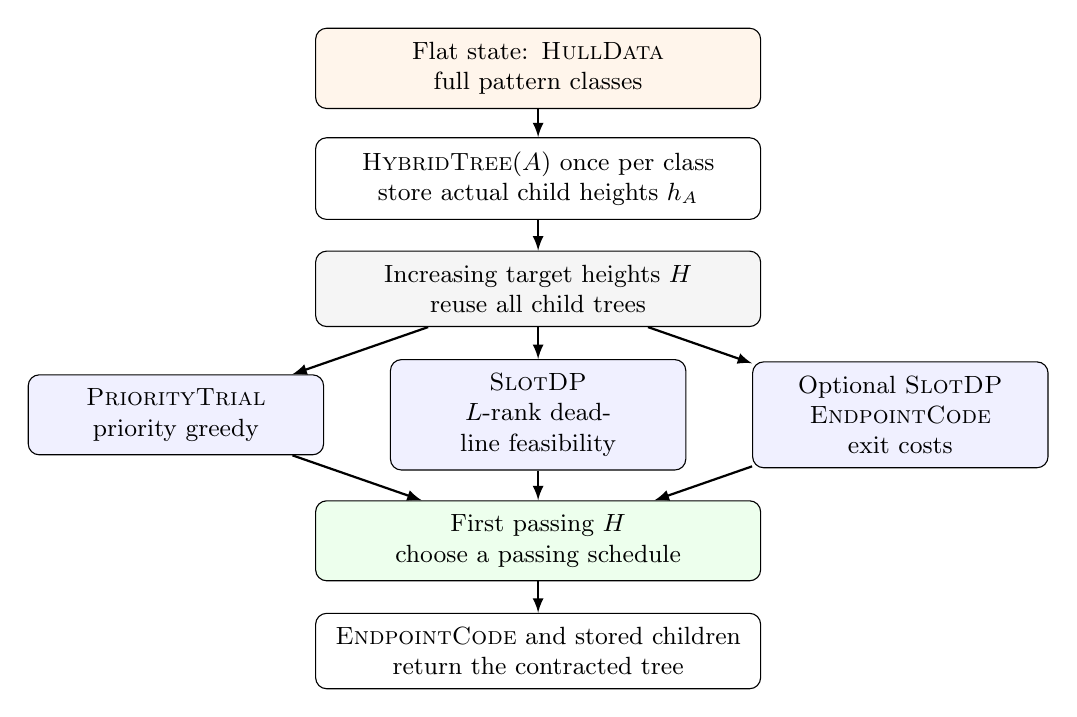
\begin{tikzpicture}[every node/.style={font=\small},
  box/.style={draw,rounded corners,align=center,inner sep=5pt,text width=3.4cm},
  wide/.style={box,text width=5.3cm},arr/.style={-latex,thick}]
  \node[wide,fill=orange!8] (hull) at (0,0)
    {Flat state: \HullData\\full pattern classes};
  \node[wide] (children) at (0,-1.4)
    {\HybridTree$(A)$ once per class\\store actual child heights $h_A$};
  \node[wide,fill=gray!8] (trial) at (0,-2.8)
    {Increasing target heights $H$\\reuse all child trees};
  \node[box,fill=blue!6] (priority) at (-4.6,-4.4)
    {\PriorityTrial\\priority greedy};
  \node[box,fill=blue!6] (slots) at (0,-4.4)
    {\SlotDP\\$L$-rank deadline feasibility};
  \node[box,fill=blue!6] (whole) at (4.6,-4.4)
    {Optional \SlotDP\\\EndpointCode\ exit costs};
  \node[wide,fill=green!7] (pass) at (0,-6)
    {First passing $H$\\choose a passing schedule};
  \node[wide] (attach) at (0,-7.4)
    {\EndpointCode\ and stored children\\return the contracted tree};
  \draw[arr] (hull) -- (children);
  \draw[arr] (children) -- (trial);
  \draw[arr] (trial) -- (priority);
  \draw[arr] (trial) -- (slots);
  \draw[arr] (trial) -- (whole);
  \draw[arr] (priority) -- (pass);
  \draw[arr] (slots) -- (pass);
  \draw[arr] (whole) -- (pass);
  \draw[arr] (pass) -- (attach);
\end{tikzpicture}
\caption{Construction of the polynomial maximum-depth tree at a flat
state. Arrows pass explicitly computed geometry, heights, or schedules.
The logarithmic cap $L$ is fixed at the original root. The priority
alternative guarantees that some height trial passes; the exact and
whole-exit alternatives can accept an earlier trial. The unknown optimum
is used only in the proof, never in this procedure.}
\label{fig:hybrid-procedure-flow}
\end{figure}



\subsection{Two simultaneous height invariants}

\begin{theorem}[General polynomial maximum-depth improvement]
\label{thm:poly-slot-worst}
For a separating supplied family of binary unit-cost planar line
queries, the hybrid algorithm runs in deterministic polynomial time
and returns a tree with
\[
 \boxed{C_W(\HH)\le(2+\gamma)\OPT_W(\HH)
       =4.46496526\,\OPT_W(\HH)<4.464966\,\OPT_W(\HH).}
\]
For a singleton input its cost is zero.
\end{theorem}
\begin{proof}
Prove simultaneously, for every recursive state of size $s$ with
$D=\OPT_W(S)$,
\begin{align}
 C_W(S)&\le3D+\lfloor\gamma\log_2s\rfloor,
                   \label{eq:slot-universal-invariant}\\
 D\le R\quad\Longrightarrow\quad
 C_W(S)&\le2D+\lfloor\gamma\log_2s\rfloor.
                   \label{eq:slot-restricted-invariant}
\end{align}
The first is the fallback guarantee; the second is stronger whenever
the exact scheduler's fixed global cap can contain the comparison
path. Both hold at singleton states.

The first follows from the proof of Theorem~\ref{thm:worst}:
its priority alternative remains available, and every hybrid child
obeys the same universal bound. Improved children only increase the
available budgets.

For the second invariant, restriction gives $\OPT_W(A)\le D$,
so every child of a state meeting $D\le R$ meets the same global
threshold. The stronger inductive bound is therefore available for
all its children. At a balanced state, both child sizes are at most
$(1-\delta)s$. Lemma~\ref{lem:worst-floor-credit} pays for the root
query, without needing the child's optimum to drop by one.

At a flat state, consider
$H^*=2D+\lfloor\gamma\log_2s\rfloor$. Write
$x=\log_2(s/|A|)$ and $\ell=\log_2(1/\delta)$.
Lemma~\ref{lem:height-prefix} gives
$\OPT_W(A)\le D-(t_A-1)$. The strong child bound implies
\begin{equation}\label{eq:slot-deadline-credit}
\begin{aligned}
 H^*-C_W(A)-z_A-5
 &\ge2(t_A-1)+\lfloor\gamma x\rfloor
                         -\lfloor x-\ell\rfloor-5\\
 &\ge2(t_A-1).
\end{aligned}
\end{equation}
The last step is the flat-state credit in
Lemma~\ref{lem:worst-floor-credit}.
Consequently $B_A+1\ge t_A$ for every nonzero class.
This is the link between restriction of an unknown optimal tree and
the deadlines computed from actual child heights.

Map each query on an optimal common-witness path to a full-hull
edge containing its one or two supporting vertices. Enlarging a
singleton support to an incident edge only accelerates hits. After
deleting repeated and unproductive blocks, every class is hit by
rank at most $t_A$. When the path terminates at an uncovered nonzero
singleton, append an incident edge; its supporting index is $q'+1$,
where $q'\le D$ is the witness-path length. This comparison has
at most $D$ blocks when the zero pattern exists and at most $D+1$
otherwise. Since $D\le R$, its length fits $L=R+1$.
For $s\ge2$, $\lfloor\gamma\log_2s\rfloor\ge2$, so also
$\lfloor H^*/2\rfloor\ge D+1$. The comparison meets both
caps in \eqref{eq:hybrid-total-cap} and every exact deadline.
Lemma~\ref{lem:rank-subset-scheduling} therefore finds a feasible
trial, and \eqref{eq:slot-block-allowance} bounds its height by $H^*$.
If the hull has dimension at most one, the at most two extreme tests
learn the pattern; the same count potential pays for them. This
proves both invariants by induction.

At the original root, if $D\le R$, use
$D\ge\log_2n$ in \eqref{eq:slot-restricted-invariant} to obtain
$C_W\le(2+\gamma)D$. If $D>R$, integrality gives
$D>\gamma q/(\gamma-1)$. Use
\eqref{eq:slot-universal-invariant} to obtain
\[
 \frac{C_W}{D}\le3+\frac{\gamma\log_2n}{D}
 <3+(\gamma-1)=2+\gamma.
\]
These cases cover all instances; the algorithm never needs $D$ as input.

Finally put $K=\gamma/(\gamma-1)=123248263/73248263$.
Since $q<\log_2n+1$, the smaller cap gives
\[
 3^L<3^{K+1}n^{K\log_2 3},\qquad
 2^L<2^{K+1}n^K,
\]
where $K<1.682611$ and $K\log_2 3<2.666874$, certified by
the rational logarithm bounds in \eqref{eq:rational-log-bounds}.
Each exact scheduling call is polynomial. There are polynomially many
trial heights and first blocks, and only $O(n)$ disjoint-child
recursive stages. Geometry, supplied-query incidence, endpoint codes,
and rational arithmetic all have polynomial cost. The final proper
tree has at most $n$ leaves and $n-1$ internal nodes.
\end{proof}

\subsection{Optimizing complete endpoint exits}

The capped scheduler can additionally optimize the actual endpoint
decoders, including their fixed recursive continuations. After a
positive answer, use the legal cut in
Section~\ref{sec:endpoint-geometry}. Each realized full pattern is
uniquely described by its left and right endpoint coordinates; supplied
hull tests are coordinate thresholds. For a rectangle $R$ of realized
endpoint pairs, give a single-class leaf $A$ value $C_W(A)$ and use
\[
 E(R)=\min_{\text{proper coordinate thresholds }\ell}
       \bigl(1+\max\{E(R\cap\ell^-),E(R\cap\ell^+)\}\bigr).
\]
Ignore empty outcomes. There are $O(M^4)$ rectangles and $O(M)$
threshold choices per rectangle. This is the exact minimum whole
height among such endpoint-comparison trees. A pinned endpoint is
its one-coordinate special case.

At a Cartesian state $([l,r],T)$, the unhit demands relevant to a
candidate block $p$ are precisely those contained in $[l,r]$.
For either block orientation, partition the classes hit by $p$
into first-endpoint-positive and second-endpoint-first-positive cells,
and precompute their complete decoder heights $E_1(l,r,p)$ and
$E_2(l,r,p)$. These cells depend only on the spatial region and the
block: an outside query cannot hit a contained interval, while an
interval crossing an ancestor was already hit. At rank $k=\min T$,
replace the fixed deadline check by
\[
 2(k-1)+1+E_1(l,r,p)\le H,\qquad
 2k+E_2(l,r,p)\le H,
\]
omitting empty-cell checks. Rank partitioning, the first circular
cut, and the total-cap test remain unchanged. For an origin or
cached endpoint these prefix bounds remain conservative.

This variant still runs in polynomial time under the same cap.
It accepts every schedule accepted by the fixed-allowance test:
the explicit dyadic endpoint codes are feasible comparison trees,
and optimal whole-height decoding only lowers their maximum height.
Thus it can be included as a third hybrid alternative without
weakening Theorem~\ref{thm:poly-slot-worst}. It improves individual
trees; a smaller universal factor is not established by this step.

\paragraph{Verification.}
The scheduler implementation compares this method with
independent exhaustive subset-permutation dynamic programs on 3,900
linear and 1,200 circular random and targeted instances. It also
rejects the fractional-only five-slot deadline example and verifies
its six-slot repair; see \texttt{further-worst-slot-}\allowbreak
\texttt{dp-check.py}. The endpoint checker compares rectangle decoding
with full subset decision-tree recursion on 1,200 weighted instances.
The theorem relies on the exact recurrence and
the two invariants above, rather than on these finite checks.
The earlier nonintegrality and forced-prefix greedy obstructions
still apply to their respective methods; they do not obstruct
rank-subset scheduling. A smaller constant from whole-exit optimization
would need a joint argument about anchors, compatible ranks, and child
heights. An endpoint-only aggregate bound is insufficient: a weighted
central cross can require four comparisons before its largest-height
continuation. Extending the cap-and-fallback argument to
arbitrary-prior expected depth needs an additional probability-weighted
tail argument: a small expected optimum can have a long witness path.

\section{Stronger algorithms for small caps}
\label{sec:small-caps}

Consider instances with a distinguished hypothesis $p$ and orient
each supplied query so that its \emph{cap} is the answer side missing
$p$. Let $P$ be the other $N$ hypotheses. These assumptions concern
the supplied queries themselves; a common external witness at a
recursive flat state is not automatically a distinguished hypothesis.
The restricted algorithms below clarify which small-cap constructions
can support approximation hardness.

\subsection{Exact maximum depth with bounded caps}

\begin{theorem}\label{thm:bounded-cap-height}
If every cap has size at most a fixed integer $b$, maximum depth is
exactly solvable in polynomial time. A running-time bound is
$m^{b-1}2^{O(b^2)}\operatorname{poly}(n,m,L)$, where $L$ is the
input bit length.
\end{theorem}
\begin{algorithm}[H]
\caption{Exact maximum depth with a distinguished miss hypothesis and bounded caps}
\label{alg:bounded-caps}
\KwIn{Distinguished hypothesis $p$; other hypotheses $P$; supplied caps of size at most fixed $b$.}
\KwOut{An exact minimum-height supplied-query tree.}
Compute the minimum supplied-halfplane cover size $K$ of $P$\;
\For{$D=K,\ldots,K+b-1$}{
  $d_0\gets\max\{0,D-b+1\}$\;
  \ForEach{ordered supplied-query suffix of length $q\le D-d_0$}{
    \ForEach{$R$ contained in the union of its caps}{
      \If{the suffix does not cover $R$}{\Continue\;}
      Find a minimum cover $Q$ of $P\setminus R$ using only caps disjoint from $R$\;
      \If{$|Q|>d_0$ or the cover is infeasible}{\Continue\;}
      Compute the suffix's first-hit groups $A_j$ on $R\cup\{p\}$\;
      \If{some $j+c_W(\ExactTree(A_j,\mathrm W))>D-d_0$}{\Continue\;}
      Execute $Q$ followed by the suffix on the all-miss spine\;
      Attach exact local supplied-query trees to all positive first-hit groups\;
      \KwRet this tree\;
    }
  }
}
\end{algorithm}

The empty suffix permits only $R=\varnothing$. Each suffix has at
most $b-1$ queries and at most $b(b-1)$ points in its union.
The minimum-cover oracle is the supplied-halfplane algorithm cited in
Theorem~\ref{thm:bounded-cap-height}; it is not the hull-interval oracle
unless that special representation is available.


\begin{proof}
Algorithm~\ref{alg:bounded-caps} gives the construction.
Let $K$ be the minimum number of supplied caps covering $P$.
Minimum planar halfplane cover is exactly solvable in polynomial
time~\cite{harpeledlee2012}. Separability ensures that the cover
exists. The path identifying $p$ in any tree must cover $P$, so
its height is at least $K$. Conversely, query a minimum cover along
the all-miss spine and identify each positive hit group locally.
A hit group has at most $b$ members and therefore admits a proper
identification tree of height at most $b-1$. This gives height at
most $K+b-1$. Only these $b$ target heights need to be tested.

For a target $D\in[K,K+b-1]$, put $d_0=\max\{0,D-b+1\}$.
Guess an ordered suffix of $q\le D-d_0\le b-1$ supplied queries
on the witness spine. Guess also the set $R\subseteq P$ remaining
just before that suffix. Require that the suffix caps cover $R$;
thus $R$ is a subset of their union and has size at most $b(b-1)$.
For each guess, compute a minimum cap cover of $P\setminus R$
using only supplied caps disjoint from $R$, and require size at
most $d_0$. An empty suffix permits $R=\varnothing$.

Execute the guessed suffix on $R\cup\{p\}$. For each nonempty
first-hit group $A_j$ at position $j$, compute its exact local
identification height $h(A_j)$ by subset Bellman DP on at most
$b$ hypotheses. Require $j+h(A_j)\le D-d_0$ and $q\le D-d_0$.
These tests verify the entire suffix tree, including the witness
leaf. The prefix cover takes at most $d_0$ queries, preserves $R$
on its all-miss route, and its positive exits cost at most $b-1$
additional queries. Thus its exits have height at most
$d_0+b-1=D$ when $d_0>0$; if $d_0=0$, the prefix is empty.
The suffix starts no later than depth $d_0$, so an accepted guess
constructs a tree of height at most $D$.

For completeness, take an optimal height-$D$ tree. If its witness
path ends before depth $d_0$, use an empty suffix and $R=\varnothing$;
its witness queries cover $P$ within $d_0$. Otherwise take the
remaining witness queries after depth $d_0$ as the suffix, and the
actual nonwitness state there as $R$. The prefix caps are disjoint
from $R$ and cover $P\setminus R$. The suffix has at most $b-1$
queries and covers $R$; its positive subtrees satisfy the exact
local-height tests. This guess is accepted. There are
$m^{O(b)}$ suffix descriptions and $2^{O(b^2)}$ candidate subsets
per suffix, and all remaining computations are polynomial for
fixed $b$. For $b=1$, a minimum cover itself is exact.
\end{proof}

\subsection{An EPTAS for weighted singleton and pair caps}

Assume every cap has size one or two, all singleton caps for $P$
are supplied, and the graph $G$ of two-point caps is a disjoint
union of paths and cycles. The latter condition follows for planar
instances with all singleton caps: every nonwitness point is a
convex-hull vertex, and a two-point cap joins consecutive vertices.
Let the positive raw weights be $w_0$ for $p$ and $w_v$ for $v\in P$,
and put $\Omega=w_0+\sum_v w_v$.

For a matching $M$, replace each matched pair by a group of mass
$w_u+w_v$ and leave unmatched vertices as singleton groups. Let
$J(M)$ be the group multiset, $k=N-|M|$, and
$P(M)=\sum_{uv\in M}(w_u+w_v)$. With group masses
$a_1\ge\cdots\ge a_k$, write $C(J)=\sum_j j a_j$. The exact
matching invoice is
\begin{equation}\label{eq:eptas-matching-invoice}
 G(M)=w_0k+C(J(M))+P(M).
\end{equation}
Indeed an arbitrary tree's first-hit groups on the witness spine
form a matching, sorted group order minimizes their weighted ranks,
and a pair exit needs one more query. Every matching is executable
using its pair tests and the supplied singleton tests. Hence
minimizing \eqref{eq:eptas-matching-invoice} gives the optimum.

\begin{theorem}\label{thm:pair-eptas}
For this weighted singleton/pair path-and-cycle class, expected
depth has a deterministic $(1+\varepsilon)$ approximation in time
$2^{O(\varepsilon^{-3})}\operatorname{poly}(n,L,\log(1/\varepsilon))$
for $0<\varepsilon\le1$. The polynomial exponent is independent
of $\varepsilon$; this is an EPTAS, not an FPTAS.
\end{theorem}
\begin{algorithm}[H]
\caption{Expected-depth EPTAS for weighted singleton/pair paths and cycles}
\label{alg:pair-eptas}
\KwIn{Distinguished miss hypothesis, supplied singleton tests and pair graph $G$;
positive raw weights; $0<\varepsilon\le1$.}
\KwOut{A deterministic $(1+\varepsilon)$ approximation.}
Set $K=\lceil3/\varepsilon\rceil$, $B=2K$,
$H=\lceil3B/\varepsilon\rceil$, and $\eta=\varepsilon/3$\;
Find the $H$ heaviest nonwitness vertices (or all of them if fewer exist)\;
\For{$r=0,\ldots,K-1$}{
  Delete edges numbered $r$ modulo $K$ on each path or cycle\;
  Enumerate each remaining component's matching configurations\;
  \ForEach{joint configuration on components meeting the heavy vertices}{
    Fix these heavy configurations\;
    Solve the light-component convex program \eqref{eq:pair-convex-relaxation}
    to raw additive accuracy $\eta\Omega$\;
    \ForEach{unfixed light component}{
      Fix a configuration minimizing the conditional expected invoice,
      using rational first and second count moments\;
    }
    Form the matched-pair and singleton groups; sort them by decreasing mass\;
    Query the supplied group tests on the miss spine,
    using one supplied singleton test to identify each pair hit\;
    Retain the resulting tree and its exact expected cost\;
  }
}
\KwRet the cheapest retained tree\;
\end{algorithm}

The component bound, heavy enumeration, convex relaxation, and
conditional-expectation guarantee are proved in
Theorem~\ref{thm:pair-eptas}. No fractional tree is output.


\begin{proof}
For $n=1$ the zero-query tree is exact, so assume $n\ge2$.
Algorithm~\ref{alg:pair-eptas} records the steps.
We work with raw weights; normalization preserves ratios. Write
$F^*=\min_M G(M)=\Omega\OPT_E$ for the optimum raw cost, where
$\OPT_E$ uses the normalized prior $w_h/\Omega$.
Set
\[
 K=\lceil3/\varepsilon\rceil,\quad B=2K,\quad
 H=\lceil3B/\varepsilon\rceil,\quad \eta=\varepsilon/3.
\]
Number edges consecutively on each path or cycle. For each common
residue $r\in\{0,\ldots,K-1\}$, delete edges numbered $r$ modulo
$K$. Each remaining component has at most $B$ vertices, allowing
the possibly longer wraparound component of a cycle.

Splitting a matched pair of weights $a\ge b$ at its original spine
position into two consecutive singleton queries changes the cost of
the temporary schedule, retaining the old group order, by exactly
$R_j-a$, where $R_j$ is the later group mass plus $w_0$.
These changes add for simultaneous splits; sorting afterward can
only decrease the cost. The sum of $R_j$ over
matched positions is at most the original tree's spine cost, hence
at most its full invoice. Every edge is deleted in exactly one
residue trial. Applying the splits to an optimal matching and then
sorting the new groups shows that some residue admits a surviving
matching of cost at most $(1+1/K)F^*$.

Order individual nonwitness weights as $w_{(1)}\ge\cdots\ge w_{(N)}$.
Because a first-hit group contains at most two vertices,
rearrangement gives
\[
 F^*\ge\sum_{i=1}^N\lceil i/2\rceil w_{(i)},\qquad
 \Omega_{\rm tail}:=\sum_{i>H}w_{(i)}
 \le\frac{2F^*}{H+1}.
\]
For each residue, enumerate all matching configurations in components
containing one of the $H$ heaviest vertices. There are at most $H$
such components and at most $2^{BH}$ joint choices. This enumeration
is independent of $n$ in its exponent. The remaining components'
total vertex mass is at most $\Omega_{\rm tail}$. If $H\ge N$,
all components are fixed and there is no rounding stage.

For a remaining component $i$, enumerate its matching configurations
$c$. A configuration supplies a group count $k_{ic}$, pair mass
$P_{ic}$, and count function $z_{ic}(t)$, the number of groups of
mass at least $t$. Choose fractional configuration weights
$x_{ic}\ge0$, $\sum_c x_{ic}=1$. For the fixed heavy components use
counts $Z_f(t)$, group count $k_f$, and pair mass $P_f$. Put
$\mu(t)=Z_f(t)+\sum_{ic}x_{ic}z_{ic}(t)$ and minimize
\begin{equation}\label{eq:pair-convex-relaxation}
 Q(x)=w_0\left(k_f+\sum_{ic}x_{ic}k_{ic}\right)
       +P_f+\sum_{ic}x_{ic}P_{ic}
       +\frac12\int_0^\infty(\mu(t)^2+\mu(t))\,dt.
\end{equation}
For any integral group multiset with count function $Z(t)$,
\[
 C(J)=\frac12\int_0^\infty(Z(t)^2+Z(t))\,dt,
\]
since the groups above each threshold occupy ranks $1$ through
$Z(t)$. Thus \eqref{eq:pair-convex-relaxation} is an exact invoice
on integral configurations and a lower-bounding convex relaxation.
Its quadratic part is a positive sum of squares of affine functions.
The only breakpoints are singleton and available-pair masses, at
most $N+|E(G)|=O(N)$ rational values. It is therefore a rational
convex quadratic program with $N2^{O(B)}$ variables over a product
of simplices. After normalizing by $\Omega$, solve it to additive
accuracy $\eta$ using polynomial-time convex quadratic
optimization~\cite{nestnem1994}. Equivalently the raw error is
$\eta\Omega$. The bounded simplices, rational coefficients, and
objective bound $O(n)$ give polynomial bit complexity and a feasible
rational approximate solution.

Independently round each light component according to its fractional
configuration distribution. Its random count $X_i(t)$ satisfies
$0\le X_i(t)\le B$ and
$\operatorname{Var}X_i(t)\le B\mathbb E X_i(t)$. Independence and
the rank integral give
\begin{align*}
 \mathbb E G(M)&=Q(x)+\frac12\int\sum_i\operatorname{Var}X_i(t)\,dt\\
 &\le Q(x)+\frac B2\Omega_{\rm tail}
 \le Q(x)+\frac{B}{H+1}F^*.
\end{align*}
The integral of a component's count function is its total group
mass, which equals its vertex mass for every configuration.
The witness and pair-continuation terms are linear, so they incur
no variance penalty. Derandomize by exposing one component at a
time and choosing a configuration with minimum conditional expected
invoice. These expectations are exact rational first and second
count moments at the same $O(n)$ breakpoints; each choice preserves
the upper bound. Sorting the final groups yields a supplied-query
tree.

For the good residue, the enumeration contains the heavy part of
an optimum surviving matching. Its fractional optimum is no greater
than that matching's invoice. Also $\Omega\le F^*$, since every
hypothesis needs at least one query in a nontrivial instance. The
returned cost is consequently at most
\[
 \left(1+\frac1K+\eta+\frac B{H+1}\right)F^*
 \le(1+\varepsilon)F^*.
\]
Dividing by $\Omega$ proves the normalized expected-depth guarantee.
Return the cheapest tree over all residues and heavy configurations.
Here $B=O(\varepsilon^{-1})$, $H=O(\varepsilon^{-2})$, so the
enumeration costs $2^{O(\varepsilon^{-3})}$; quadratic optimization
and derandomization have polynomial exponent independent of
$\varepsilon$. All-singleton availability is essential both for the
invoice's converse and for the splitting construction.
\end{proof}

The EPTAS includes the weighted pair-path instances in the
expected-depth hardness reduction below. Its exponential dependence
on $1/\varepsilon$ is compatible with strong NP-completeness.
It rules out using this subclass to
establish APX-hardness unless $\mathrm P=\mathrm{NP}$.

\section{A PTAS for uniform shallow caps in convex position}
\label{sec:uniform-cap-ptas}

The bounded-cap restriction also permits an approximation scheme for
uniform expected depth when the hypotheses are in convex position.
The construction first clears short gaps in their cyclic order.
Every remaining query then acts inside one bounded-size block.
A count-vector dynamic program retains all choices of how to interleave
queries from these blocks. Uniform weights make blocks with the same
local test family interchangeable.

\begin{theorem}\label{thm:uniform-cap-ptas}
Suppose $\HH=P\cup\{p\}$ is in strictly convex position, $p$ is a
distinguished hypothesis, and every supplied side missing $p$ contains
at most a fixed number $b\ge1$ of hypotheses. Under the uniform prior,
expected depth admits a polynomial-time approximation scheme. Every
query in the returned tree is supplied; singleton caps need not be
available.

More explicitly, for $0<\varepsilon\le1$, put
\[
 \ell=\max\left\{2b,\ b(b-1),\
                 \left\lceil\frac{8b^2}{\varepsilon}\right\rceil\right\},
 \qquad d_{b,\ell}=2^{(b+1)\ell}.
\]
One running-time bound is
$f(b,\ell)(n+1)^{d_{b,\ell}}\operatorname{poly}(n,m,L)$, where
$L$ is the input bit length and $f$ depends only on $b,\ell$.
The polynomial exponent depends on $b$ and $\varepsilon$; the
guarantee is a PTAS.
\end{theorem}

\begin{proof}
Write $N=|P|=n-1$ and work with the raw uniform cost
$G(T)=\sum_{h\in\HH}d_T(h)$; dividing by $n$ preserves ratios.
Write $\OPT_G=\min_TG(T)=n\OPT_E$.
When $N<\ell$, exact subset Bellman optimization is sufficient,
since the state size depends only on $b$ and $\varepsilon$.
Assume henceforth that $N\ge\ell$.

\paragraph{Clear gaps between small blocks.}
Each cap is a cyclic interval in the convex order of $P$: a line
crosses the boundary of its convex polygon at most twice. Partition
that order into consecutive pieces of length $\ell$, with a possibly
shorter last piece. Mark the first $b$ points of each piece, or the
whole piece when its size is at most $b$. Let $D$ be the marked set
and $r=|D|$. Then
\begin{equation}\label{eq:uniform-cap-deletion-count}
 r\le b\lceil N/\ell\rceil\le\frac{2bN}{\ell}.
\end{equation}
The unmarked portions are blocks of at most $\ell$ points. Between
neighboring nonempty blocks, including across the cyclic wraparound,
there are at least $b$ marked points. A cyclic cap of size at most $b$
cannot meet two such blocks, because it would also contain an entire
intervening gap and hence at least $b+2$ points.

While a marked point $x$ remains on the miss spine, query any supplied
cap containing $x$. Such a cap exists because the supplied tests
distinguish $x$ from $p$. Identify its first-hit group by a proper
local supplied-query tree, and continue on the miss side. Separation
gives a local height at most $|A|-1\le b-1$ for each hit group $A$:
repeatedly query a line separating two remaining hypotheses. Each
spine query clears a new marked point, so at most $r$ are used.
Additional unmarked points may leave through these exits. The
residual portions of the blocks still have size at most $\ell$, and
every residual cap lies in one block.

The prefix's spine nodes cost at most $r(N+1)$ in total. At most
$br$ points leave through its hit exits, each with at most $b-1$
additional local queries. Thus the complete prefix contribution is
\begin{equation}\label{eq:uniform-cap-prefix-cost}
 G_{\rm prefix}\le r(N+1)+b(b-1)r\le2r(N+1),
\end{equation}
using $N\ge\ell\ge b(b-1)$.

\paragraph{Optimize all block interleavings exactly.}
Relabel the points of each residual block by their positions. Its
type $T$ is its size together with the family $\mathcal F_T$ of all
distinct nonempty supplied-query masks on that block. No cap can
wrap around a block's ends, since it would contain an entire marked
gap. Deleting additional points preserves interval order. Thus every
mask is an ordinary interval of at most $b$ positions. Padding to
$\ell$ positions gives at most $b\ell$ possible masks, hence at most
$2^{b\ell}$ families. The union of a family's masks is its full block,
since every point is separated from $p$, so the family also determines
the block size. A local
state $(T,R)$ records a nonempty live mask $R$ in a block of type $T$.
There are at most $d_{b,\ell}$ local states. Let $c_{T,R}$ count the
blocks in each state, and let
\[
 W(c)=1+\sum_{T,R}c_{T,R}|R|
\]
be the total live mass, including $p$. Uniformity ensures that these
counts retain all information needed to optimize the continuation.

For each type, precompute by Algorithm~\ref{alg:exact-tree} the exact
raw local cost $g_T(A)$ of identifying every subset $A$ using its
supplied masks. Here the positive branch has no distinguished
witness, and $g_T(A)=0$ for $|A|\le1$. Let $e_{T,R}$ be a unit count
vector, with $e_{T,\varnothing}=0$. The exact miss-continuation
recurrence is
\begin{equation}\label{eq:uniform-cap-count-dp}
 \begin{aligned}
 F(0)&=0,\\
 F(c)&=W(c)+\min_{\substack{c_{T,R}>0,\ q\in\mathcal F_T\\
                          A=R\cap q\ne\varnothing}}
 \left\{g_T(A)+F\bigl(c-e_{T,R}+e_{T,R\setminus A}\bigr)\right\}.
 \end{aligned}
\end{equation}
Every transition removes a live point, so the recurrence is acyclic.
At any proper query, its hit group lies in one block and its miss
branch retains $p$ and the other blocks. The positive subtree can be
optimized locally, giving precisely the recurrence's lower bound
for every adaptive tree. Conversely, a transition chooses a physical
block of the specified type and live mask, and an original supplied
query realizing $q$. That query misses every other residual block.
Its stored local positive code and miss continuation realize the
recurrence. Backtracking therefore reconstructs a legal identifying
tree, including all choices of block interleaving.

Each count lies between zero and $N$, giving at most
$(N+1)^{d_{b,\ell}}$ states. Local Bellman tables and the transitions per
state depend only on $\ell$, and constructing the types takes
polynomial time in the input. All raw costs are integral and at most
$n(n-1)$, so their bit complexity is polynomial.

\paragraph{Charge the prefix against the optimum.}
Restrict an optimal full tree to the residual hypotheses, suppressing
constant-answer nodes. Restriction can only decrease depths, so the
exact residual cost from \eqref{eq:uniform-cap-count-dp} is at most
$\OPT_G$. On the other hand, the witness spine of any full tree has
first-hit groups of size at most $b$, and hence
\begin{equation}\label{eq:uniform-cap-rank-lower}
 \OPT_G\ge\sum_{i=1}^N\lceil i/b\rceil
          \ge\frac{N(N+1)}{2b}.
\end{equation}
Combining \eqref{eq:uniform-cap-prefix-cost},
\eqref{eq:uniform-cap-deletion-count}, and
\eqref{eq:uniform-cap-rank-lower} gives
\[
 \frac{G_{\rm alg}-\OPT_G}{\OPT_G}
 \le\frac{4br}{N}
 \le\frac{8b^2}{\ell}
 \le\varepsilon.
\]
Dividing by $n$ proves the expected-depth guarantee.
\end{proof}

\begin{algorithm}[H]
\caption{Uniform expected-depth PTAS for bounded convex-position caps}
\label{alg:uniform-cap-ptas}
\KwIn{Uniform hypotheses $P\cup\{p\}$ in convex position; supplied
caps missing $p$, each of size at most fixed $b$; $0<\varepsilon\le1$.}
\KwOut{A supplied-query tree of expected cost at most
$(1+\varepsilon)\OPT_E$.}
$N\gets|P|$;
$\ell\gets\max\{2b,b(b-1),\lceil8b^2/\varepsilon\rceil\}$\;
\If{$N<\ell$}{\KwRet $\ExactTree(P\cup\{p\},\mathrm E)$ with raw unit weights\;}
Partition the convex cyclic order of $P$ into pieces of length
$\ell$; mark their first $\min\{b,\text{piece size}\}$ points as $D$\;
$U\gets P$; start an empty miss-spine prefix\;
\While{$D\cap U\ne\varnothing$}{
 Choose $x\in D\cap U$ and a supplied cap $q$ containing $x$\;
 $A\gets U\cap q$\;
 Append $q$ to the prefix; attach a legal local code for $A$
 of height at most $|A|-1$ on its hit side\;
 $U\gets U\setminus A$; continue on the miss side\;
}
Intersect the unmarked pieces with $U$ to obtain the residual blocks\;
Store each physical block's map from its masks to realizing supplied
queries; group identical mask families as types $T$ and compute every
local cost $g_T(A)$ by \ExactTree\;
Compute the initial count vector $c$ of the full residual block masks\;
Evaluate \eqref{eq:uniform-cap-count-dp}, memoizing minimizing transitions\;
Backtrack from $c$: select a physical block in the chosen state,
query that block's stored realizing line, and translate the local
positive code using the same block's query map\;
Attach the reconstructed continuation to the prefix's miss leaf\;
\KwRet the resulting tree\;
\end{algorithm}

The proof uses only the cyclic-interval property of the caps. In
particular it also applies when the nonwitness points alone are in
convex position. For fixed $b$, a constant-factor hardness reduction
through uniform one-layer shallow-cap instances would contradict
this PTAS unless $\mathrm P=\mathrm{NP}$. A construction based on
bounded-size caps must therefore prove interactions beyond this
cyclic-interval subclass to establish such a gap.

\section{Allowing hypotheses on supplied lines}
\label{sec:boundaries}

Algorithm~\ref{alg:boundary} implements the reduction below.
In this section a supplied line returns one of three answers:
negative, zero, or positive. The \emph{zero}, or \emph{on-line},
answer means the hypothesis lies on the queried line, and its
answer class is $S_\ell^0=\{h\in S:f_\ell(h)=0\}$.
A \emph{ternary decision tree} has an outgoing edge for each
possible answer; a proper such tree retains only nonempty outcomes.
Leaf depths and the two cost objectives are defined exactly as
in the binary model.
Use the two virtual binary predicates
\[
 b_1(h)=\mathbf1[f_\ell(h)<0],\qquad
 b_2(h)=\mathbf1[f_\ell(h)\le0].
\]
Their pair of bits distinguishes the three outcomes.
Requesting either bit is implemented by querying the original line
once and storing its full sign. Both bits are then known. For analysis
we count each requested virtual bit as a separate binary query;
the actual number of supplied-line queries can only be smaller.

These binary labelings have planar off-boundary representations.
Any query whose answer is constant on the hypothesis set can be
discarded. For every remaining query, choose $\epsilon_\ell$ to be
half the minimum nonzero $|f_\ell(h)|$ on the finite hypothesis set.
This rational value is computable in polynomial time and has
polynomial encoding length. Then $b_1$ is represented
by $f_\ell(x)<-\epsilon_\ell$ and $b_2$ by
$f_\ell(x)<\epsilon_\ell$. Neither shifted boundary contains a
hypothesis. The shifts are used only for preprocessing;
their answers are obtained from the original supplied line.

\begin{symboltable}
$f_\ell(h)$ & Affine value whose sign is the answer for hypothesis $h$.\\
$b_1(h),\ b_2(h)$ & Virtual bits for $f_\ell(h)<0$ and $f_\ell(h)\le0$; together they encode the ternary sign.\\
$\epsilon_\ell$ & Positive shift smaller than every nonzero $|f_\ell(h)|$ for this finite state.
\end{symboltable}

\begin{algorithm}[H]
\caption{Transfer a binary algorithm to on-line outcomes}
\label{alg:boundary}
\KwIn{Finite hypotheses, supplied ternary lines, binary tree-construction routine $B$.}
\KwOut{An executable tree using the original supplied lines.}
\ForEach{nonconstant supplied line $\ell$}{
  $\epsilon_\ell\gets\frac12\min_{h:f_\ell(h)\ne0}|f_\ell(h)|$\;
  Represent virtual bits $b_1=\mathbf1[f_\ell(h)<0]$ and
  $b_2=\mathbf1[f_\ell(h)\le0]$ by the two shifted off-boundary lines\;
}
Construct a virtual binary tree with $B$\;
Execute a requested virtual bit by querying its original line,
caching the entire ternary sign; answer further requests from that cache\;
\KwRet the contracted original-line tree\;
\end{algorithm}

Lines constant on the whole hypothesis set are discarded before taking
the minimum nonzero affine value. Proposition~\ref{prop:boundary}
proves that the approximation ratio increases by at most two.


\begin{proposition}[Boundary reduction]\label{prop:boundary}
An $\alpha$-approximation for either binary objective gives a
$2\alpha$-approximation for the corresponding three-answer objective.
\end{proposition}
\begin{proof}
Simulate every query of an optimal original tree by its two virtual
bits. Each hypothesis uses at most twice as many binary queries,
so the virtual optimum is at most twice the original optimum
for either objective. Conversely, execute a constructed virtual
tree by original line queries and cached signs. Its actual depth
is no larger than its virtual depth on every hypothesis.
The two comparisons prove the factor-two transfer.
\end{proof}

\begin{corollary}[Constant approximations with on-line outcomes]
\label{cor:constant-boundaries}
With on-line answers, expected depth has a polynomial-time
approximation factor below $10.365952$ for arbitrary positive priors,
and deterministic maximum depth has a factor below $8.929931$.
\end{corollary}
\begin{proof}
Apply Proposition~\ref{prop:boundary} to
Theorems~\ref{thm:two-phase-expected} and~\ref{thm:poly-slot-worst}.
\end{proof}

\section{Strong NP-completeness}
\label{sec:hardness}

The approximation algorithms exploit planar structure, but exact
optimization remains hard. We first state the decision and source
problems and the graph terminology used by both reductions.

\begin{definition}[Complexity and reductions]\label{def:complexity}
A \emph{polynomial-time many-one reduction} maps instances of one
decision problem to another in polynomial time, so an input is a
yes-instance if and only if its image is a yes-instance.

A decision problem is in \emph{NP} if every yes-instance has a
certificate of polynomial encoding length whose validity is
checkable in polynomial time, and no certificate is accepted on a
no-instance. It is \emph{NP-hard} if every problem
in NP admits such a reduction to it, and \emph{NP-complete} if it
is both NP-hard and in NP.
A numerical problem is \emph{strongly NP-hard} if hardness persists
when its integer data are bounded by a fixed polynomial in the
combinatorial instance size; it is \emph{strongly NP-complete} if
it is also in NP. For rational data, our restricted instances
explicitly bound both numerators and denominators.
\end{definition}

\begin{definition}[3-Partition]\label{def:three-partition}
The input consists of positive integers $a_1,\ldots,a_m,B$, where
$m=3p$ for a positive integer $p$, satisfying
\[
 s=\sum_{i=1}^m a_i=pB,\qquad B/4<a_i<B/2.
\]
The question is whether $[m]$ can be partitioned into $p$ groups
$I_1,\ldots,I_p$ with $|I_b|=3$ and
$\sum_{i\in I_b}a_i=B$ for every $b$.
\end{definition}

\begin{symboltable}
$m=3p,\ [m]$ & Number of source items and their index set.\\
$a_i,\ B$ & Item size $i$ and target sum of each bin.\\
$s=pB=\sum_i a_i$ & Total item size and total capacity of the $p$ bins.\\
$I_b$ & Index set of the three items assigned to source bin $b$.\\
\end{symboltable}

Both reductions use the strong NP-completeness of this
problem~\cite{gj1979}.
We use the NP-hard restriction in which $B$ is polynomially bounded
in $m$. The case $p=1$ is a trivial yes-instance, so excluding it
preserves NP-hardness. In this restriction each $a_i$ is
polynomially bounded, so the explicit
repetitions in our constructions remain polynomial in the source
size. A partition into $p$ groups of sum $B$
then necessarily has three items per group: two items sum to less
than $B$, while four items sum to more than $B$.

\begin{definition}[Paths and matchings]\label{def:paths-and-matchings}
A \emph{path} is an undirected graph with distinct vertices
$v_0,\ldots,v_k$ and edges exactly
$\{v_{j-1},v_j\}$ for $1\le j\le k$.
A \emph{linear forest} is a disjoint union of paths, allowing
isolated vertices. In this paper an \emph{odd path} has an odd
number of vertices, not an odd number of edges.
Odd and even positions refer to local positions numbered from zero
along an item path, not to global hypothesis indices.

A \emph{matching} is a set of edges with no shared endpoint.
A vertex is \emph{unmatched} if it is incident to no chosen edge.
A \emph{maximum matching} has largest possible cardinality;
``maximum'' here always refers to the number of edges, not their
weights. A \emph{perfect matching} leaves no vertex unmatched.
\end{definition}

The two reductions share a combinatorial mechanism. They place each
item on an odd path and supply singleton and adjacent-pair membership
tests. A maximum matching leaves one even-position vertex unmatched;
its position chooses the item's bin. Moving that position changes
a short part of a histogram. The maximum-depth reduction counts
branch heights, while the expected-depth reduction counts pair weights.
In both cases these local changes add to the source bin loads.

\subsection{The geometric realization and the matching choice}

For integer abscissae, the line
\[
 I_{a,b}:\quad
 4y-4(a+b)x+(2a-1)(2b+1)=0
\]
has value $4(x-a+\tfrac12)(x-b-\tfrac12)$ on $(x,x^2)$.
Its negative answer selects exactly the integer abscissae
$a,\ldots,b$. This realizes interval membership using one line.
The line
\begin{equation}\label{eq:private-singleton}
 P_t:\quad 2y-4tx+2t^2-1=0
\end{equation}
has value $2(x-t)^2-1$, and its negative answer isolates exactly
the point of abscissa $t$. Both formulas are nonzero at all integer
abscissae, so every answer is binary.
The tangent $y=2tx-t^2$ exposes the point $(t,t^2)$, since every
other parabola point lies strictly above it. The constructed
hypotheses are therefore in strictly convex position.

In both reductions, membership sets are the negative answer classes
of the displayed lines. Thus a hit in
Definition~\ref{def:membership-spine} is the negative affine sign;
the distinguished hypothesis misses these sets. The query itself
is unchanged.



These formulas provide the two query types needed by the reduction:
an interval query selects a consecutive block, and a private
singleton query distinguishes one point from all the others.
Putting the points on a parabola gives both query types with integer
coefficients while keeping every hypothesis exposed on the convex
hull. For example, Figure~\ref{fig:parabola-queries} shows
$I_{2,5}$ and $P_4$ on the points with integer abscissae from $0$ to $8$.

\begin{figure}[tbp]
\centering
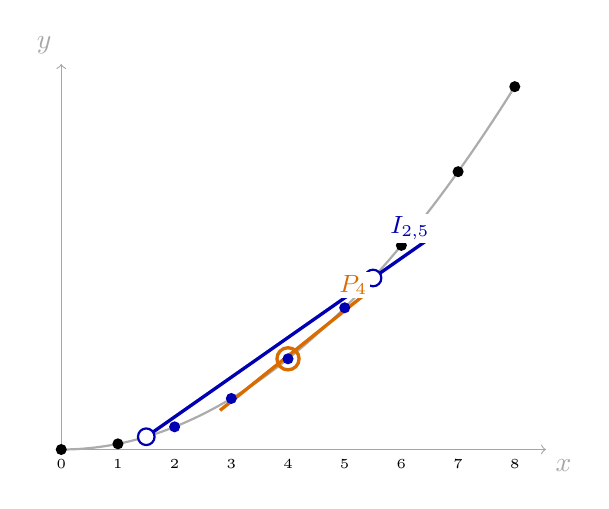
\begin{tikzpicture}[x=0.72cm,y=0.072cm]
  \draw[->,gray!70] (0,0)--(8.55,0) node[below right] {$x$};
  \draw[->,gray!70] (0,0)--(0,68) node[above left] {$y$};
  \foreach \x in {0,...,8} {
    \node[below,font=\tiny] at (\x,0) {\x};
  }
  \draw[thick,gray!65] plot[domain=0:8,samples=81] (\x,{(\x)^2});
  \draw[very thick,blue!70!black]
    plot[domain=1.5:6.5,samples=60] (\x,{7*\x-8.25});
  \draw[very thick,orange!85!black]
    plot[domain=2.8:5.4,samples=50] (\x,{8*\x-15.5});
  \draw[blue!70!black,fill=white,thick] (1.5,2.25) circle (3pt);
  \draw[blue!70!black,fill=white,thick] (5.5,30.25) circle (3pt);
  \foreach \x in {0,1,6,7,8} {
    \pgfmathsetmacro{\yy}{\x*\x}
    \fill[black] (\x,\yy) circle (2pt);
  }
  \foreach \x in {2,3,4,5} {
    \pgfmathsetmacro{\yy}{\x*\x}
    \fill[blue!70!black] (\x,\yy) circle (2pt);
  }
  \draw[orange!85!black,very thick] (4,16) circle (4pt);
  \node[font=\small,text=blue!70!black,fill=white,inner sep=1pt]
    at (6.15,39) {$I_{2,5}$};
  \node[font=\small,text=orange!85!black,fill=white,inner sep=1pt]
    at (5.15,29) {$P_4$};
\end{tikzpicture}
\caption{The integer points lie on $y=x^2$. The blue line
$I_{2,5}$ has negative answer exactly on the points with
$x\in\{2,3,4,5\}$; the orange line $P_4$ has negative answer only
at $x=4$, marked with an orange ring. The interval endpoints are
the half-integer intersections $x=1.5$ and $x=5.5$.}
\label{fig:parabola-queries}
\end{figure}

For maximum depth we also use \emph{clouds} of ordinary points.
They make a local identification problem take a chosen number of
queries without changing the objective. A cloud's size $w_i$ is
its number of points, not a prior weight.
Given positive integer cloud sizes $w_i$, put $Q=4\max_i w_i$
and represent cloud $i$ by
\[
 \{(Qi+j,(Qi+j)^2):0\le j<w_i\}.
\]
Its point with $j=0$ is its \emph{anchor}. Supply the cloud-interval line
\begin{equation}\label{eq:cloud-interval}
 4y-4Q(a+b)x+Q^2(2a-1)(2b+1)=0.
\end{equation}
For $a\ge1$ its negative answer selects exactly the clouds
$a,\ldots,b$, while excluding cloud $0$.
This follows by factoring its value as
$4(x-Q(a-\tfrac12))(x-Q(b+\tfrac12))$.
Each cloud lies within $Q/4$ of its anchor, so neither boundary,
halfway between consecutive anchors, contains a hypothesis.
We supply private lines \eqref{eq:private-singleton} for each
nonanchor point, but not for the anchors. An anchor and a point
in its own cloud agree on every cloud-interval test and on every
other private test. Their separation requires that point's
private query. Thus a cloud of size $w$ forces $w-1$ queries on
the anchor's local path, while the anchor itself remains available
to represent the cloud in the matching construction.

Clouds are ordered so that consecutive vertices of each path used
below have consecutive cloud indices. The only cloud-interval tests
are whole-cloud singleton tests and adjacent-pair tests specified
by those paths. Every point, including every anchor, must be identified.

\begin{lemma}[Identifying one or two clouds]\label{lem:cloud-heights}
For this supplied family, the minimum height on one cloud of size $w$
is $w-1$. On two clouds of sizes $u,v$, when their whole-cloud
singleton tests are supplied, the minimum height is $\max\{u,v\}$.
\end{lemma}
\begin{proof}
On a single cloud, old cloud-interval tests are constant and each
private test isolates one nonanchor point. The anchor answers the
same way as every nonanchor on all the other private tests, so its
path must ask all $w-1$ of them. Querying them sequentially achieves
that height.

On two clouds, the anchor of the larger cloud must use all its
private tests: each is the only query separating that cloud's anchor
from its corresponding nonanchor. It must also use at least one
cloud-interval test, since private tests give the same answer at
both anchors. The larger cloud therefore forces depth at least
$\max\{u,v\}$.
First separating the clouds and then performing their private
searches attains the bound.
\end{proof}

\begin{lemma}[One unmatched position]\label{lem:odd-path}
A maximum matching of the path
\[
 E_0,B_1,E_1,\ldots,B_t,E_t
\]
leaves exactly one vertex $E_k$ unmatched. It then uses pairs
$\{E_{j-1},B_j\}$ for $j\le k$ and
$\{B_j,E_j\}$ for $j>k$.
\end{lemma}
\begin{proof}
The maximum size is $t$, so exactly one vertex is unmatched.
Both sides of that vertex must have even length, forcing it
to be an $E_k$. Each remaining even path has a unique perfect
matching: its endpoint must match its only neighbor, and induction
fixes the rest. This gives the displayed pairs.
\end{proof}

Figure~\ref{fig:odd-path-matching} shows the smallest nontrivial
example of the matching pattern. Moving the unmatched even-position
cloud changes which segment represents the item's bin choice.
\begin{figure}[tbp]
\centering
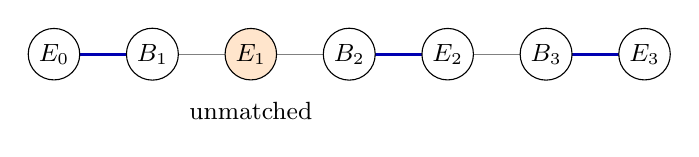
\begin{tikzpicture}[every node/.style={font=\small}]
  \draw[gray] (0,0)--(7.5,0);
  \draw[very thick,blue!70!black] (0,0)--(1.25,0);
  \draw[very thick,blue!70!black] (3.75,0)--(5,0);
  \draw[very thick,blue!70!black] (6.25,0)--(7.5,0);
  \node[draw,circle,fill=white,inner sep=2pt] at (0,0) {$E_0$};
  \node[draw,circle,fill=white,inner sep=2pt] at (1.25,0) {$B_1$};
  \node[draw,circle,fill=orange!20,inner sep=2pt] at (2.5,0) {$E_1$};
  \node[draw,circle,fill=white,inner sep=2pt] at (3.75,0) {$B_2$};
  \node[draw,circle,fill=white,inner sep=2pt] at (5,0) {$E_2$};
  \node[draw,circle,fill=white,inner sep=2pt] at (6.25,0) {$B_3$};
  \node[draw,circle,fill=white,inner sep=2pt] at (7.5,0) {$E_3$};
  \node[below=14pt] at (2.5,0) {unmatched};
\end{tikzpicture}
\caption{A maximum matching of
$E_0,B_1,E_1,B_2,E_2,B_3,E_3$ with $E_1$ left unmatched.
Blue edges are the selected adjacent pairs. In the reduction, the
unmatched even-position cloud selects the item's bin; the uniquely
forced pairs lie to its left and right.}
\label{fig:odd-path-matching}
\end{figure}

The item paths only organize the supplied membership queries. The
reduction uses singleton and adjacent-pair tests directly; no
underlying edge-query search tree is part of the instance.

\subsection{Maximum depth: bin loads become branch-height counts}

The construction has three jobs. A distinguished anchor forces the
spine to use a maximum matching. Only a few small even-position
clouds can be left unmatched, giving exactly $p$ bin choices per
item. Finally, the heights of the matched pairs record how much
load was assigned to each bin.

\begin{theorem}[Strong NP-completeness of maximum depth]
\label{thm:strong-worst}
Deciding whether $\OPT_{\mathrm W}(\HH)\le K$ is strongly NP-complete,
even for integer-coordinate points on a parabola, polynomially
bounded integer line coefficients, and $O(n)$ supplied binary
line queries.
\end{theorem}
\begin{proof}
For the source instance define
\[
 \begin{split}
 q&=(p-1)(4s+2m),\qquad M=m+2,\qquad K=q+M,\\
 T&=s-B,\qquad
 \lambda_1=M,\qquad
 \lambda_b=M+(2b-3)s\quad(2\le b\le p),\\
 H&=M+2s(p-1),\qquad C=H+1.
 \end{split}
\]
Here $q$ will be the total number of matched pairs and $K$ the
minimum length of the distinguished anchor's path.
The numbers $\lambda_b$ mark histogram levels for bins, and
$T$ is the width of each bin's window. The larger sizes $H,C$
keep the remaining pairs above those windows.

\begin{symboltable}
$q,\ K$ & Total number of matched pairs in a maximum matching and target maximum depth.\\
$M=m+2$ & Auxiliary-cloud size and offset used for the minimum bin level.\\
$T=s-B,\ \lambda_b$ & Width of each bin's histogram window and its lower level.\\
$H,\ C=H+1$ & Higher pair and connector exit heights, above every bin window.\\
$s_i=(p-1)(4a_i+2)$ & Number of odd-position clouds, and maximum matching size, in item $i$'s path.\\
\end{symboltable}

For item $i$, construct an odd path whose vertices represent clouds.
Starting with an even-position cloud of size $2$, append $p-1$
segments, indexed by $b=1,\ldots,p-1$. Each row below appends an
odd-position cloud and then the next even-position cloud.
Segment $b$ consists of one entry row, $a_i$ repetitions of the
four block rows, and one exit row:
\[
 \begin{array}{c|c|c}
 \text{part}&\text{odd-position size}&\text{next even size}\\ \hline
 \text{entry}&C&M\\
 \text{block step 1}&\lambda_b&H\\
 \text{block step 2}&\lambda_b+T&M\\
 \text{block step 3}&\lambda_{b+1}+T&H\\
 \text{block step 4}&\lambda_{b+1}&M\\
 \text{exit}&C&2
 \end{array}
\]
The repeated block is the only part depending on $a_i$.
It transfers $a_i$ units between neighboring histogram windows.
There are $4a_i+2$ odd-position vertices per segment, so the
whole item path has $2s_i+1$ vertices, where
$s_i=(p-1)(4a_i+2)$, and its maximum matching has size $s_i$.
Its $p$ even-position clouds of size $2$ are the segment boundaries.

Add one auxiliary cloud of size $M$ and cloud $0$ of size $2$.
Supply each nonzero cloud's whole-cloud singleton test, each
adjacent-pair test within an item path, and each nonanchor point's
private singleton test. Realize them by \eqref{eq:cloud-interval}
and \eqref{eq:private-singleton}.

\paragraph{Step 1: a tight distinguished path forces a matching.}
\begin{claim}[The distinguished path forces maximum matchings]
Every identifying tree has height at least $K$. If its height is at
most $K$, the first-covered pairs form a maximum matching in every
item path, and no nonzero-cloud private test is asked on the anchor
path.
\end{claim}
\begin{proof}
Follow the anchor of cloud $0$ through any complete tree. It needs the private
test for the other point of cloud $0$. Private tests of other
clouds do not distinguish their anchors from this anchor.
It therefore also needs cloud queries covering the $2q+m$ item-path
anchors and the auxiliary anchor.

Classify each anchor by its first hitting cloud query along this
all-miss path. A query first covers one anchor or two adjacent
anchors. The first-covered pairs are disjoint, hence form a
matching of size at most $\sum_i s_i=q$.
There are $2q+m+1$ nonzero anchors to cover. If $g$ first-covered
groups are pairs, the remaining groups are singletons, so the path
uses $(2q+m+1)-g$ cloud queries. Since $g\le q$, this is at least
$q+m+1$. It must also ask the private query separating the two
points of cloud $0$, giving the lower bound
$q+m+2=K$.

If a tree has height at most $K$, equality holds. No private test
of a nonzero cloud can occur on this path, and its pairs form a
maximum matching in every item path. Lemma~\ref{lem:odd-path}
therefore leaves exactly one even-position cloud unmatched per item.
\end{proof}

At this equality, all clouds are intact when first encountered:
none of their private points was removed earlier. A hit exit
contains one full cloud or two full clouds.
Replace any query first covering just one cloud by its supplied
whole-cloud singleton test. Put cloud $0$'s private query last;
this advances the other exits and leaves its two points within
depth $K$. Attach the optimal local codes of
Lemma~\ref{lem:cloud-heights}.

\paragraph{Step 2: summarize the remaining tree by a histogram.}
\begin{claim}[The sorted exit profile characterizes depth]
After the cloud-query groups are sorted by nonincreasing local
height, every target path has depth at most $K$ exactly when
$t+N(t)\le K$ at every exit-height level $t$.
\end{claim}
\begin{proof}
The cloud queries now act on disjoint singletons and pairs.
Their exit heights are $w-1$ for a singleton and $\max\{u,v\}$
for a pair. Include the final private query as an exit of height
zero. Sorting these heights in nonincreasing order cannot hurt:
exchanging consecutive heights $r<s$ replaces
$\max\{j+r,j+1+s\}$ by $\max\{j+s,j+1+r\}$.

Write $h_j$ for the local height of the exit at spine position $j$.
The \emph{tail histogram} of exit heights is
$N(t)=|\{j:h_j\ge t\}|$, the number of exits of height at least $t$.
In sorted order, the last such exit occurs at position $N(t)$.
An exit at position $j$ with local height $h_j$ has total depth
$j+h_j$. Because the heights are sorted, the maximum of these sums
is exactly the maximum of $t+N(t)$ over exit-height levels $t$:
an exit of height $t$ occurs no later
than position $N(t)$, and the last exit counted by $N(t)$ has height
at least $t$. Thus all target paths fit within $K$ exactly when
\begin{equation}\label{eq:height-profile}
 t+N(t)\le K
\end{equation}
for every exit-height level $t$.
This criterion is simply the maximum of ``spine position plus
remaining local depth.''
\end{proof}

\paragraph{Step 3: only boundaries are feasible unmatched positions.}
\begin{claim}[Height feasibility forces a bin boundary]
In any tree of height at most $K$, the unmatched even-position
cloud in each item path is one of its $p$ boundary clouds.
\end{claim}
\begin{proof}
Every matched pair has exit height at least $M$, because each odd
cloud has size at least $\lambda_1=M$. The auxiliary singleton has exit
height $M-1$. An unmatched internal even vertex has size $M$ or $H$,
and hence exit height at least $M-1$.
At $t=M-1$, these give
$N(t)\ge q+1+\text{number of such internal unmatched vertices}$.
Since $K=q+M$, \eqref{eq:height-profile} excludes all of them.
The unmatched vertex in each item path therefore chooses one of
its $p$ boundary positions, interpreted as a bin.
\end{proof}

\paragraph{Step 4: moving a boundary transfers the item's load.}
Let $L_b$ be the sum of the item numbers choosing bin $b$ and put
\[
 Q_{\mathrm{hi}}=2(p-1)(s+m),\qquad
 \beta_1=q-s,\qquad
 \beta_b=Q_{\mathrm{hi}}+2s(p-b)\quad(2\le b\le p).
\]
\begin{claim}[Histogram windows record the bin loads]
At the upper level $t_b=\lambda_b+T$ of bin window $b$,
\[
 N(t_b)=\beta_b+L_b,\qquad t_b+\beta_b=K-B.
\]
Thus the height profile requires $L_b\le B$ for every bin.
\end{claim}
\begin{proof}
To see the transfer, compare the two matchings on segment $b$.
When its unmatched vertex is before the segment, a repeated block
has heights
\[
 H,\ \lambda_b+T,\ H,\ \lambda_{b+1}.
\]
When that vertex is after the segment, the same block has heights
\[
 \lambda_b,\ H,\ \lambda_{b+1}+T,\ H.
\]
The two connector pairs have height $C$ in either case.
With $a_i$ repetitions, the change in $N(t)$ is exactly
\[
 -a_i\mathbf1_{(\lambda_b,\lambda_b+T]}(t)+
  a_i\mathbf1_{(\lambda_{b+1},\lambda_{b+1}+T]}(t).
\]
The windows are disjoint because $T<s$ and consecutive
$\lambda_b$ differ by at least $s$.
Moving across several segments cancels the intermediate transfers:
an item assigned to bin $b$ removes $a_i$ from window 1 and
adds $a_i$ to window $b$. Figure~\ref{fig:hardness-window-transfer}
illustrates this change relative to the reference matching.

In the reference matching assigning all items to bin 1,
$Q_{\mathrm{hi}}$ pairs have height $H$ or $C$.
For each segment $b$, the other pairs include $s$ of height
$\lambda_b+T$ and $s$ of height $\lambda_{b+1}$.
At thresholds in the first window, the reference tail count is
$q=\beta_1+s$. For a later window $b$, the reference tail count is
$Q_{\mathrm{hi}}+2s(p-b)=\beta_b$: the $Q_{\mathrm{hi}}$ high pairs
always count, and each later segment contributes $2s$ lower pairs.
At the upper window level $t_b=\lambda_b+T$, the transfer formula
therefore gives
\[
 N(t_b)=\beta_b+L_b,\qquad t_b+\beta_b=K-B.
\]
The profile condition at this level is
$t_b+N(t_b)\le K$, or equivalently $L_b\le B$.
Thus \eqref{eq:height-profile} requires $L_b\le B$ for every bin.
Since $\sum_b L_b=s=pB$, all these inequalities are equalities
and yield a source 3-partition.
\end{proof}

\paragraph{Step 5: a source partition gives a complete tree.}
\begin{claim}[A source partition gives height at most $K$]
If the source items are partitioned into bins of load $B$, there is
a complete identifying tree of height at most $K$.
\end{claim}
\begin{proof}
Choose the boundary matchings of a source partition, so $L_b=B$.
The window upper levels satisfy \eqref{eq:height-profile} with equality.
For completeness, the remaining levels have the following counts:
\[
 \begin{array}{c|c|c}
 t&N(t)&t+N(t)\\ \hline
 0&K&K\\
 1&K-1&K\\
 M-1&q+1&K\\
 \lambda_b&\beta_b+s&K\\
 H&Q_{\mathrm{hi}}&K\\
 C&2m(p-1)&K-2s(p-1)+1\le K
 \end{array}
\]
These are all possible exit heights, together with the already
checked $\lambda_b+T$. The count $N(t)$ is constant between
successive exit heights, so $t+N(t)$ increases there and its maximum
occurs at a listed exit height. Sort the corresponding queries, attach
their exact one- or two-cloud codes, and finish with cloud $0$'s
private query. This constructs a complete tree of height $K$.
\end{proof}

\paragraph{Size and encoding.}
There are $2q+m+2$ clouds, each of size at most
$C=O(ps+m)$. Their total number of hypotheses is polynomial in
the restricted source input. The realization has integer coordinates
and line coefficients bounded by $O(n^4)$, with $O(n)$ supplied
lines. Every proper identifying tree has $n-1$ internal nodes;
its answers and height can be checked in polynomial time.
This proves membership in NP and strong NP-hardness with
polynomially bounded numerical data.
\end{proof}

\begin{figure}[tbp]
\centering
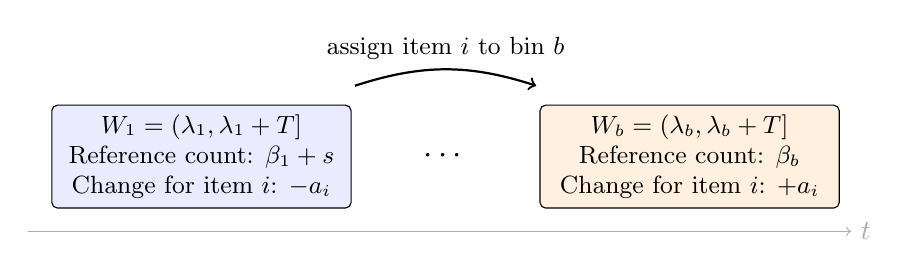
\begin{tikzpicture}[
  window/.style={draw,rounded corners=2pt,minimum width=3.8cm,
                 minimum height=1.15cm,align=center,font=\small}
]
  \node[window,fill=blue!8] (windowone) at (0,0)
    {$W_1=(\lambda_1,\lambda_1+T]$\\
     Reference count: $\beta_1+s$\\
     Change for item $i$: $-a_i$};
  \node[font=\large] at (3.1,0) {$\cdots$};
  \node[window,fill=orange!12] (windowb) at (6.2,0)
    {$W_b=(\lambda_b,\lambda_b+T]$\\
     Reference count: $\beta_b$\\
     Change for item $i$: $+a_i$};
  \draw[->,thick] (1.95,0.9) to[bend left=18]
    node[above,font=\small] {assign item $i$ to bin $b$}
    (4.25,0.9);
  \draw[->,gray!65] (-2.2,-0.95)--(8.25,-0.95)
    node[right] {$t$};
\end{tikzpicture}
\caption{Relative to the reference matching, assigning one item of
size $a_i$ from bin 1 to bin $b$ removes $a_i$ from the first
histogram window and adds $a_i$ to window $b$; intermediate windows
are unchanged. Superposing the item transfers gives
$N(t)=\beta_j+L_j$ throughout window
$W_j=(\lambda_j,\lambda_j+T]$.}
\label{fig:hardness-window-transfer}
\end{figure}

\subsection{Expected depth: an exact matching formula}

The expected-depth reduction needs no clouds. Each nonzero
hypothesis is one path vertex or one isolated vertex, and every
query isolates either a singleton or an adjacent pair.
The combinatorial choice is still a matching, but its objective
depends on how the resulting pairs are ordered.

For a finite positive weight vector $z$, keeping repeated values
as distinct entries, define the \emph{weighted completion sum} by
\[
 \mathcal C(z)=\sum_{j=1}^{|z|}jz_{(j)},
 \qquad z_{(1)}\ge\cdots\ge z_{(|z|)}.
\]
It equals the sum of the individual weights plus the smaller
weight for each unordered pair of entries: in decreasing order,
an earlier entry delays a later entry by one. Thus concatenating
vectors $u,v$ adds the cross contribution
$\sum_{i,j}\min\{u_i,v_j\}$.
Equivalently,
if $h_z(t)=|\{j:z_j\ge t\}|$, then
\begin{equation}\label{eq:completion-histogram}
 \mathcal C(z)=\int_0^\infty
                 \frac{h_z(t)(h_z(t)+1)}2\,dt.
\end{equation}
At height $t$, the first $h_z(t)$ ranks contribute
$1+\cdots+h_z(t)$; integrating those contributions proves the identity.

\begin{lemma}[Exact singleton/pair formula]\label{lem:pair-invoice}
Consider a \emph{linear forest}, meaning a disjoint union of paths
(isolated vertices are allowed), with vertices $1,\ldots,N$ ordered
component by component. Represent them and a distinguished hypothesis by
$(i,i^2)$, $0\le i\le N$. Supply $I_{i,i}$ for each nonzero vertex
and $I_{i,i+1}$ for each forest edge.
Give the distinguished hypothesis weight $\omega_0>0$ and the
others positive weights $\omega_v$.
For a matching $\mathcal M$, let $J(\mathcal M)$ be the vector
containing mass
$\omega_u+\omega_v$ for each matched pair and $\omega_v$ for each
unmatched vertex, retaining multiplicities when masses coincide.
The optimal unnormalized expected depth is
\begin{equation}\label{eq:pair-invoice}
 \min_{\mathcal M}
 \left\{\omega_0(N-|\mathcal M|)
       +\mathcal C(J(\mathcal M))
       +\sum_{\{u,v\}\in\mathcal M}(\omega_u+\omega_v)\right\}.
\end{equation}
If $\omega_0>N\sum_{v>0}\omega_v$, an optimal matching in this
formula has maximum cardinality.
\end{lemma}
\begin{proof}
Follow hypothesis $0$, which misses every supplied membership query.
The hypotheses first covered together are disjoint singletons
or adjacent pairs. The pairs form a matching $\mathcal M$,
and the spine has $N-|\mathcal M|$ queries.
A pair's hit branch requires exactly one additional query;
a singleton branch requires none.
This gives the first and third terms of \eqref{eq:pair-invoice}.

For the first-cover term, suppose masses $a<b$ occupy consecutive
positions $j,j+1$. Their contribution is
$ja+(j+1)b$ in that order and $jb+(j+1)a$ after swapping, a decrease
of $b-a$. Repeated exchanges show that nonincreasing mass is optimal.
Every such ordering is executable: query the selected pairs
and the singleton tests for the unmatched vertices in that order.
The groups are disjoint, so each query's hit branch exits only
to its own group. This proves the
formula both as a lower bound on arbitrary trees and as an
attainable value for each matching.

Every proper complete tree has depth at most $N$, so the total
weighted depth of all nonzero hypotheses is at most
$N\sum_{v>0}\omega_v$. One additional query on hypothesis $0$'s
path outweighs this entire budget under the stated inequality.
An optimal tree must consequently minimize that path's length,
which means choosing a maximum-cardinality matching.
\end{proof}

\subsection{Expected depth: bin loads become a quadratic penalty}

The formula above separates three effects: the distinguished
point's depth, first-cover positions, and one extra query for
each pair. We will force a maximum matching by making the
distinguished point sufficiently likely. Pair weights then
record the bin loads in disjoint histogram windows.
Small adjustments to the unmatched boundary weights cancel the
histogram's unwanted linear terms, leaving a quadratic penalty.

\begin{theorem}[Strong NP-completeness of expected depth]
\label{thm:strong-average}
Given supplied binary lines, a prior obtained by normalizing
strictly positive integer weights bounded by a fixed polynomial in
$n$, and a rational threshold $K$, deciding whether
$\OPT_{\mathrm E}(\HH)\le K$ is strongly NP-complete.
This holds for $\HH=\{(i,i^2):0\le i<n\}$, $O(n)$ supplied lines
with polynomially bounded integer coefficients, and even when each
query's negative class contains at most two hypotheses.
\end{theorem}
\begin{proof}
We again reduce from the restricted 3-Partition input.
In this proof put
\[
 q=2s(p-1),\qquad
 \beta_1=q-s,\qquad
 \beta_b=2s(p-b)\quad(2\le b\le p),\qquad
 a_{\max}=\max_i a_i.
\]
The integer $q$ is again the total matching size.
The $\beta_b$ will be the baseline pair counts in the bin windows.
Choose the explicit polynomial integers
\[
 \begin{split}
 r&=1000\bigl[(p+10)(q+m+1)^2
             +(qmp+2m+1)\beta_1a_{\max}+1\bigr],\\
 V&=2000m(r+q+m+1),\qquad Z=V/2,\qquad t_i=q+r+m-i,\\
 \delta_{ib}&=\left\lfloor
          \frac{V(\beta_1-\beta_b)a_i}{t_i}\right\rfloor,\qquad
 D=\max_{i,b}\delta_{ib},\qquad A_i=1+(2D+1)i,\\
 \lambda_b&=(10+2b)V\quad(1\le b\le p).
 \end{split}
\]
\begin{symboltable}
$q,\ \beta_b$ & Total matching size and baseline pair count in bin window $b$.\\
$r,\ V,\ Z=V/2$ & Number of medium-weight isolated hypotheses, window width, and isolated-hypothesis weight.\\
$t_i$ & Coefficient with which item $i$'s unmatched boundary weight contributes to the expected-depth objective.\\
$\delta_{ib},\ D$ & Boundary adjustment for item $i$ in bin $b$, and the largest such adjustment.\\
$A_i$ & Increasing base weight for item $i$'s unmatched boundary hypothesis.\\
$\lambda_b$ & Lower level of bin window $b$, separated from neighboring windows by $2V$.\\
$b_i,\ L_b$ & Bin assigned to item $i$ and total item size assigned to bin $b$.\\
$U_i,\ z,\ G$ & Unmatched item weights, matched-pair masses, and the resulting unnormalized weighted depth.\\
$G_{\mathrm{fix}},\ C_{\mathrm{ref}},\ e$ & Matching-independent cost, reference completion sum, and bounded rounding/perturbation error.\\
$E_+,\ E_-,\ k_0,\ k$ & Upper and lower error bounds, baseline threshold, and final decision threshold.\\
\end{symboltable}
For $b\ge2$,
$\beta_1-\beta_b=(2b-3)s>0$, so all $\delta_{ib}$ are
nonnegative; the formula gives $\delta_{i1}=0$.
The even-position vertices $E_{i,2a_i(b-1)}$ are the $p$ boundary
choices for item $i$; leaving boundary $b$ unmatched assigns that
item to bin $b$. Between consecutive boundaries are $2a_i$ steps,
with $a_i$ increases and $a_i$ decreases in the even weights.
The odd weights are chosen so the two possible pairings at an
increasing step have masses $\lambda_b$ and $\lambda_b+V$, while
those at a decreasing step have masses $\lambda_{b+1}+V$ and
$\lambda_{b+1}$. Moving the unmatched position across a segment
therefore transfers exactly $a_i$ pair masses from bin window $b$
to window $b+1$.

This transfer is the encoding invariant. The large window width $V$
makes a unit of load imbalance dominate all rounding errors. The
small boundary adjustments $\delta_{ib}$ will cancel the remaining
linear dependence on the chosen bins, leaving a quadratic penalty
that is zero exactly for a 3-partition.
The constants $1000$ and $2000$ provide slack in the scale
estimates below. The combinatorial information is carried by
the item lengths and the bin windows, not by those constants.

\paragraph{Step 1: construct the weighted item paths.}
For item $i$, form an odd path
\[
 E_{i0},\,B_{i1},\,E_{i1},\,\ldots,\,
 B_{is_i},\,E_{is_i},\qquad s_i=2a_i(p-1),
\]
where each displayed symbol also denotes that vertex's weight.
First define unperturbed even weights
\[
 E^0_{ij}=
 \begin{cases}
 A_i,&j\equiv0\pmod{2a_i},\\
 A_i+V,&j\text{ odd},\\
 A_i+2V,&\text{otherwise}.
 \end{cases}
\]
Each consecutive difference is $+V$ or $-V$.
Between two boundary positions there are $2a_i$ steps,
of which $a_i$ go up and $a_i$ go down.
For $1\le j\le s_i$ let $b=\lceil j/(2a_i)\rceil$ and put
\[
 B_{ij}=
 \begin{cases}
 \lambda_b-E^0_{i,j-1},&E^0_{ij}-E^0_{i,j-1}=V,\\
 \lambda_{b+1}-E^0_{ij},&E^0_{ij}-E^0_{i,j-1}=-V.
 \end{cases}
\]
Finally set
$E_{i,2a_i(b-1)}=A_i+\delta_{ib}$ at each of the $p$ boundaries
and leave all other even weights unperturbed.
The odd weights do not change when this adjustment is made.

Add $r$ isolated forest vertices of weight $Z$.
The nonzero forest has $N=2q+m+r$ vertices, with maximum matching
size $q$. Let $P$ be the total weight of its item-path vertices,
$W=P+rZ$, and give hypothesis $0$ weight
$\omega_0=(N+1)W+1$.
Use precisely the lines of Lemma~\ref{lem:pair-invoice}.
Normalize the weights only after the construction.

\paragraph{Step 2: verify the separation between weight scales.}
\begin{claim}[The chosen parameters separate the weight scales]
\begin{equation}\label{eq:expected-scale-bounds}
 \begin{split}
 \max_{i,b}(A_i+\delta_{ib})&<V/100,\\
 E_+ :=q\sum_{i,b}\delta_{ib}&\le V/1000,\\
 E_- :=\sum_i(t_i-1)&<V/2000.
 \end{split}
\end{equation}
\end{claim}
\begin{proof}
Indeed, $t_i\ge r$ gives $D\le V\beta_1a_{\max}/r$.
Consequently,
\[
 E_+\le qmpD\le V/1000,
 \qquad
 \max_{i,b}(A_i+\delta_{ib})
 \le(2m+1)D+m+1
 \le V/1000+V/2000<V/100.
\]
The bound $m+1\le V/2000$ follows directly from
$V=2000m(r+q+m+1)$.
Also $t_i-1<r+q+m+1$, giving
$E_-<m(r+q+m+1)=V/2000$.
\end{proof}
The first bound keeps every boundary singleton below $Z$ and fixes
the order of the unmatched item weights. The second limits the total
change in pair-mass completion cost caused by the perturbations; the
third bounds the accumulated error from the floors. The large $r$
is chosen to make all three estimates hold with room to spare.

Every even weight is positive. By the first bound in
\eqref{eq:expected-scale-bounds}, $A_i+\delta_{ib}<V/100$, so
$A_i+2V<2.01V$ and every unmatched even weight is below $3V$.
For an upward step, the two possible pair masses are
$\lambda_b$ and $\lambda_b+V$; for a downward step they are
$\lambda_{b+1}+V$ and $\lambda_{b+1}$. Since
$\lambda_b\ge12V$ and $\lambda_{b+1}\ge14V$, all these masses are
at least $12V$. Boundary adjustments are nonnegative and can only
increase a matched pair's mass. The odd weights are also positive:
each is either $\lambda_b-E^0_{i,j-1}$ or
$\lambda_{b+1}-E^0_{ij}$, and every unperturbed even weight is
less than $2.01V$. Hence every pair mass exceeds $Z=V/2$ and every
unmatched even weight.
Lemma~\ref{lem:pair-invoice} restricts the optimum to maximum
matchings. By Lemma~\ref{lem:odd-path}, each item then leaves
one even vertex unmatched.

\paragraph{Step 3: isolate the matching-dependent terms.}
Write $U=(U_1,\ldots,U_m)$ for the unmatched weights and $z$ for
the $q$ pair masses. Their exact weighted depth is
\begin{claim}[Expected-depth invoice for a fixed matching]
\begin{equation}\label{eq:expected-remaining-invoice}
 G=G_{\mathrm{fix}}+\mathcal C(z)+\mathcal C(U)
       +(q-1)\sum_i U_i+r\sum_i\min\{U_i,Z\},
\end{equation}
where
\[
 G_{\mathrm{fix}}=
 \omega_0(q+m+r)+\frac{Zr(r+1)}2+qrZ+P.
\]
\end{claim}
\begin{proof}
To derive this expression, split the completion sum into the
three groups $z,U$, and the $r$ isolated weights $Z$.
Since every pair mass is larger than the other weights, their
cross terms are $qrZ$ and $q\sum_iU_i$.
The remaining cross term is $r\sum_i\min\{U_i,Z\}$.
Identifying the pairs adds their total weight
$P-\sum_iU_i$, which changes the coefficient $q$ to $q-1$.
The distinguished path contributes $\omega_0(q+m+r)$.
Everything not depending on the matching is collected in
$G_{\mathrm{fix}}$.
\end{proof}

\paragraph{Step 4: compute what a boundary choice changes.}
\begin{claim}[Pair-mass windows encode the bin loads]
Let $b_i$ be the bin chosen by item $i$ and
$L_b=\sum_{i:b_i=b}a_i$. Let $z^0$ be the unperturbed pair-mass
vector for these choices, and let $C_{\mathrm{ref}}$ be the
completion sum of the reference vector in which every item chooses
bin $1$. Then
\begin{equation}\label{eq:expected-bin-identity}
 \mathcal C(z^0)=C_{\mathrm{ref}}+
 V\left[\sum_b\beta_bL_b-\beta_1s+
             \frac{\sum_bL_b^2-s^2}{2}\right].
\end{equation}
\end{claim}
\begin{proof}
Unmatching boundary $2a_i(b-1)$ assigns item $i$ to bin $b$.
Temporarily omit the boundary perturbations and denote the
resulting pair-mass vector by $z^0$.
For an upward step in segment $b$, pairing its odd vertex
to the even vertex on the left gives mass $\lambda_b$,
while pairing right gives $\lambda_b+V$.
For a downward step, those masses are
$\lambda_{b+1}+V$ and $\lambda_{b+1}$.
Moving the unmatched vertex across a whole segment consequently
changes the pair-mass histogram by
\[
 -a_i\mathbf1_{(\lambda_b,\lambda_b+V]}+
  a_i\mathbf1_{(\lambda_{b+1},\lambda_{b+1}+V]}.
\]
There are exactly $a_i$ steps of each type.
As in the maximum-depth construction, transfers across consecutive
segments cancel except at the starting and chosen bins.
In the reference matching, all odd vertices are paired to their
right. Segment $b$ contributes $s$ masses $\lambda_b+V$ and
$s$ masses $\lambda_{b+1}$ after summing over items.
For thresholds $t$ in the first window, the reference tail count
is $q=\beta_1+s$; for later window $b$ it is
$2s(p-b)=\beta_b$. Assigning items according to loads $L_b$
changes the tail count throughout window $b$ to
$\beta_b+L_b$: the first window loses $s-L_1$ pair masses from its
reference count $q$, while each later window gains $L_b$.
Outside these disjoint windows the tail histogram is unchanged.

Let $C_{\mathrm{ref}}$ be the completion sum of the unperturbed
pair masses when every first boundary is unmatched. It is explicitly
computable by sorting those $q$ masses.
Within a window the integrand of
\eqref{eq:completion-histogram} is the triangular polynomial
$h(h+1)/2$. Substituting $h=\beta_b+L_b$ and subtracting the
reference loads $(s,0,\ldots,0)$ gives the following expression.
For a baseline count $\beta_b$, the change in the triangular
polynomial is
$\beta_bL_b+(L_b^2+L_b)/2$. The reference has load $s$ in the first
window, so its change is
$\beta_1s+(s^2+s)/2$. Subtracting this reference change cancels the
linear $L_b/2$ terms because $\sum_bL_b=s$.
The remaining expression has a useful quadratic term, but also
the unwanted linear term $\sum_b\beta_bL_b$.
\end{proof}

\paragraph{Step 5: cancel the linear term and bound rounding.}
\begin{claim}[Boundary adjustments leave only a bounded error]
For every boundary matching, there is an error $e$ with
$-E_-\le e\le E_+$ such that
\begin{equation}\label{eq:expected-quadratic-gap}
 G=G_{\mathrm{fix}}+\sum_i t_iA_i+C_{\mathrm{ref}}+
       \frac V2\left(\sum_bL_b^2-s^2\right)+e.
\end{equation}
\end{claim}
\begin{proof}
Boundary perturbations increase pair masses by at most the total
added boundary weight. For a vector $z$ of $q$ pair masses,
$\mathcal C(z)=\min_\sigma\sum_{j=1}^q jz_{\sigma(j)}$, by the
adjacent-swap ordering argument in Lemma~\ref{lem:pair-invoice}.
If coordinates increase by a total
amount $\Delta$, this representation shows that $\mathcal C$ is
nondecreasing and increases by at most $q\Delta$: evaluate the new
vector in an ordering optimal for the old one. Here
$\Delta\le\sum_{i,b}\delta_{ib}$, so the increase is at most
$q\sum_{i,b}\delta_{ib}=E_+$.
All boundary unmatched weights are below $Z$, and their order is
the fixed decreasing item order. Indeed,
$A_{i+1}-(A_i+D)=D+1>0$, so even the largest perturbation of item
$i$ leaves it below the unperturbed weight of item $i+1$.
Thus their terms in \eqref{eq:expected-remaining-invoice} are
$\sum_i t_i(A_i+\delta_{ib_i})$.
Indeed, item $i$ has rank $m-i+1$ in $\mathcal C(U)$, plus
coefficient $q-1+r$ from the other terms, giving $t_i=q+r+m-i$.
The floor definition gives
\[
 -E_-\le
 \sum_i t_i\delta_{ib_i}
       -V\sum_i(\beta_1-\beta_{b_i})a_i
 \le0.
\]
For each item, the difference is minus the remainder when the
integer $V(\beta_1-\beta_{b_i})a_i$ is divided by $t_i$; its
magnitude is therefore at most $t_i-1$.
Its intended contribution
$V\sum_i(\beta_1-\beta_{b_i})a_i$ cancels the unwanted linear
term in \eqref{eq:expected-bin-identity}.
Each floor loses an integer between zero and $t_i-1$.
Combining that loss with the pair-mass increase gives
the claimed error interval.
\end{proof}

\paragraph{Step 6: distinguish exact balance by a quadratic gap.}
\begin{claim}[The quadratic gap detects a 3-partition]
For boundary choices, the threshold $k$ is met exactly when every
bin load is $B$.
\end{claim}
\begin{proof}
Define the integer threshold
\[
 k_0=G_{\mathrm{fix}}+\sum_i t_iA_i+C_{\mathrm{ref}}+
              \frac V2(pB^2-s^2),\qquad k=k_0+E_+.
\]
Because $\sum_bL_b=pB$,
\[
 \sum_bL_b^2-pB^2=\sum_b(L_b-B)^2.
\]
A source partition makes this sum zero and gives weighted depth
at most $k$. Otherwise the integral deviations sum to zero and
include at least one positive and one negative entry. Their
squares sum to at least two.
The weighted depth is then at least $k_0+V-E_-$.
The scale bounds give
$V-E_->1999V/2000>V/1000\ge E_+$, so this depth exceeds
$k=k_0+E_+$.
\end{proof}

\paragraph{Step 7: exclude internal unmatched vertices.}
\begin{claim}[An internal unmatched vertex exceeds the threshold]
Every maximum matching that leaves an internal even-position item
vertex unmatched has weighted depth greater than $k$.
\end{claim}
\begin{proof}
The preceding calculation concerned boundary choices. To complete
soundness, a maximum matching leaving an internal even vertex
unmatched must also exceed $k$.
Such a vertex has weight $A_i+V$ or $A_i+2V$, exceeding $Z$.
Every other unmatched weight is at least its $A_i$.
Its interactions with the $r$ isolated vertices contribute $rZ$
instead of at least $rA_i$. The other matching-dependent terms
in \eqref{eq:expected-remaining-invoice} are nonnegative, so
\[
 G\ge G_{\mathrm{fix}}+r\sum_i A_i+
                   r\bigl(Z-\max_i A_i\bigr).
\]
On the other hand, $pB^2-s^2\le0$ gives
\[
 k\le G_{\mathrm{fix}}+r\sum_i A_i+
           C_{\mathrm{ref}}+(q+m)\sum_i A_i+E_+.
\]
The reference masses are at most $(11+2p)V$, so
$C_{\mathrm{ref}}\le(p+6)(q+1)^2V$.
Using $A_i<V/100$, the last three terms are less than
$(p+8)(q+m+1)^2V$.
But $Z-\max_i A_i>V/3$ and
$r\ge1000(p+10)(q+m+1)^2$.
The lower bound for an internal unmatched vertex is therefore
strictly larger than $k$.
\end{proof}
Thus the medium-weight isolated hypotheses exclude all internal
choices. Soundness now covers every maximum matching, and
Lemma~\ref{lem:pair-invoice} makes this sufficient for arbitrary
adaptive trees.

\paragraph{Size, positive priors, and membership in NP.}
Normalize the positive weights by their total $\Omega$ and use
the expected-depth threshold $k/\Omega$.
The construction has polynomial size on the restricted source input.
With $n=N+1$, we have $V=O(n^2)$, all nonzero vertex weights are
$O(n^3)$, and $\omega_0=O(n^5)$.
Coordinates and supplied-line coefficients are $O(n^2)$ and there
are $O(n)$ queries. Membership in NP follows by evaluating a
proper complete tree with $n-1$ internal nodes.
Both the normalized priors and the threshold have polynomially
bounded integer numerators and denominators. This establishes
strong NP-completeness with strictly positive polynomially bounded
hypothesis weights.
\end{proof}


\section{Uniform expected-depth hardness}
\label{sec:uniform-hardness}

The weighted reduction of Section~\ref{sec:hardness} also yields
uniform-prior hardness, but a direct replacement of a weight by
ordinary points requires a normalization argument. We prove an exact
replacement theorem. It preserves the weighted optimum up to a
computable additive term, despite the additional private queries.
Throughout this section, raw uniform cost means the sum of the leaf
depths, before division by the number of hypotheses.

\subsection{A rotation for a private singleton}

\begin{lemma}[Uniform singleton rotation]\label{lem:uniform-singleton-rotation}
Suppose a proper identifying tree on a uniformly weighted state $S$
first asks a supplied query isolating $x\in S$, and the other child
first asks a query $r$ that is proper on $S\setminus\{x\}$.
These two queries can be exchanged, placing the singleton query
in the answer branch of $r$ containing $x$, without increasing
the raw cost.
\end{lemma}
\begin{proof}
Let $A,B$ be the two nonempty answer classes of $r$ on
$S\setminus\{x\}$, and choose their names so that $x$ has the
answer of $A$. In the original tree, $x$ has relative depth one
and every hypothesis in $A\cup B$ passes through both queries.
Ask $r$ first, put the private singleton query in its
$A\cup\{x\}$ branch, and attach the original subtrees on $A$ and
$B$. The depth of $x$ increases by one, the depth of every point
of $B$ decreases by one, and all other depths are unchanged.
The change in raw cost is $1-|B|\le0$. The resulting queries are
proper and are members of the original supplied family.
\end{proof}

If the two queries isolate different singleton points, the same
rotation has zero cost. The lemma concerns equal weights; it
does not assert the corresponding inequality for unequal priors.

\subsection{An exact geometric cloud replacement}

Consider the weighted singleton/pair linear forest instance of
Lemma~\ref{lem:pair-invoice}, with vertices $0,1,\ldots,N$ and
positive integer weights $w_0,\ldots,w_N$. Vertex $0$ is
distinguished. Order the nonzero vertices along each path and
component by component, so every edge joins consecutive indices. Define
\[
 n=\sum_{i=0}^N w_i,\qquad Q=4\max_i w_i,\qquad
 C_i=\{(Qi+j,(Qi+j)^2):0\le j<w_i\}.
\]
The point with $j=0$ is the anchor of cloud $C_i$.
For every nonzero vertex supply its whole-cloud singleton query;
for every linear forest edge supply its whole-cloud pair query.
For consecutive cloud indices $a,\ldots,b$, these are the negative
answers of
\begin{equation}\label{eq:uniform-cloud-membership}
 4y-4Q(a+b)x+Q^2(2a-1)(2b+1)=0.
\end{equation}
The value on the parabola factors as
$4(x-Q(a-\tfrac12))(x-Q(b+\tfrac12))$.
Every cloud has width less than $Q/4$, so the negative answer
selects exactly those clouds and excludes cloud $0$.

For every nonanchor point of abscissa $t$, including those of
cloud $0$, supply the private line
\[
 2y-4tx+2t^2-1=0.
\]
Its value on $(x,x^2)$ is $2(x-t)^2-1$; its negative answer
isolates precisely that point. No private line is supplied for
an anchor. All answers are strict and binary.
The whole-cloud singleton queries separate the anchors, and
the private lines distinguish every nonanchor, so the family
identifies every hypothesis. All hypotheses have uniform prior $1/n$.

Put
\begin{equation}\label{eq:uniform-cloud-offset}
 D(w)=\frac{(w-1)(w+2)}2,\qquad
 \Delta=\sum_{i=0}^N D(w_i).
\end{equation}
Algorithm~\ref{alg:uniform-cloud-lift} gives the construction and
the threshold conversion.

\begin{algorithm}[H]
\caption{Uniform cloud replacement of a weighted linear forest instance}
\label{alg:uniform-cloud-lift}
\KwIn{Vertices $0,\ldots,N$ with each path in order, component by component,
positive integer weights $w_i$, and a raw weighted threshold $k$}
\KwOut{Supplied-line instance with uniform prior and threshold
$(k+\Delta)/n$}
$Q\gets4\max_i w_i$; $n\gets\sum_iw_i$;
$\HH\gets\varnothing$; $\LL\gets\varnothing$\;
\For{$i=0,\ldots,N$}{
  \For{$j=0,\ldots,w_i-1$}{
    $t\gets Qi+j$; add $(t,t^2)$ to $\HH$\;
    \If{$j>0$}{
      Add $2y-4tx+2t^2-1=0$ to $\LL$\;
    }
  }
}
For each $i>0$, add \eqref{eq:uniform-cloud-membership}
with $(a,b)=(i,i)$ to $\LL$\;
For each linear forest edge $\{i,i+1\}$, add
\eqref{eq:uniform-cloud-membership} with $(a,b)=(i,i+1)$ to $\LL$\;
$\Delta\gets\sum_{i=0}^N(w_i-1)(w_i+2)/2$\;
\KwRet $(\HH,\LL)$, prior $1/n$, and threshold $(k+\Delta)/n$\;
\end{algorithm}

\begin{lemma}[Local uniform cloud costs]\label{lem:uniform-cloud-local}
The optimal raw local cost on one intact cloud of size $w$ is
$D(w)$. On two intact clouds of sizes $u,v$, it is
\[
 D(u)+D(v)+u+v.
\]
\end{lemma}
\begin{proof}
Within one cloud, every whole-cloud query is constant, and every
nonconstant query isolates one of its nonanchors. The only possible
proper code is a chain, whose sum of depths is
$1+2+\cdots+(w-1)+(w-1)=D(w)$; for $w=1$ the sum is zero.

On two clouds a nonconstant whole-cloud query separates the
clouds, attaining the displayed formula. Every other nonconstant
query isolates one nonanchor. Induct on $u+v$.
If a private point of the $u$ cloud is queried first, the
remaining two-cloud state has sizes $u-1,v$ and still has its
anchors and whole-cloud separator. Using induction, this choice
costs
\[
 u+v+D(u-1)+D(v)+(u-1)+v.
\]
Subtracting $D(u)+D(v)+u+v$ gives $v-1\ge0$, because
$D(u)-D(u-1)=u$.
The analogous difference for a private point of the $v$ cloud
is $u-1\ge0$. The base case $u=v=1$ has raw cost two.
When one size is one it has no private point, and the same
induction applies to the other cloud. Queries selecting other
clouds are constant or separate these two whole clouds, so the
argument covers the entire supplied family.
\end{proof}

\begin{theorem}[Exact uniform cloud transfer]\label{thm:uniform-cloud-transfer}
Let $\OPT_{\mathrm{raw}}^{\mathrm{weighted}}$ be the minimum
raw weighted cost of the singleton/pair linear forest instance.
For its uniform cloud replacement,
\begin{equation}\label{eq:uniform-cloud-transfer}
 n\OPT_{\mathrm E}^{\mathrm{cloud}}
   =\OPT_{\mathrm{raw}}^{\mathrm{weighted}}+\Delta.
\end{equation}
Equivalently, if $J(\mathcal M)$ has the pair and singleton masses
from Lemma~\ref{lem:pair-invoice}, the raw uniform optimum is
\[
 \Delta+\min_{\mathcal M}
 \left\{w_0(N-|\mathcal M|)
   +\mathcal C(J(\mathcal M))
   +\sum_{\{u,v\}\in\mathcal M}(w_u+w_v)\right\}.
\]
\end{theorem}
\begin{proof}
Start with a proper optimal uniform tree and follow the anchor
of cloud $0$. Suppose a private query for a nonanchor $x$ of a
nonzero cloud occurs on this path. Its own cloud anchor is still
on the path, since no private query isolates an anchor.
Repeatedly apply Lemma~\ref{lem:uniform-singleton-rotation} to
move this private query past the next query on the anchor-$0$
path. The next query is proper on the remaining state; constant
queries have already been removed. Private queries commute
at zero cost. Eventually a whole-cloud query separates $x$'s
anchor from the anchor of cloud $0$: otherwise the tree would
not identify both anchors. The point $x$ has the answer of its
own anchor to that query. After the rotation its private query
is in the hit branch, off the anchor-$0$ path.

Each such operation removes one external private query from
that path, introduces none, and moves it through only finitely
many existing path queries. Repetition therefore terminates.
Next commute each cloud-$0$ private query past all remaining
whole-cloud queries. Its point always has the answer of the
anchor of cloud $0$, so it stays on that path but moves after
the last whole-cloud query. This second process also terminates,
by decreasing the number of private/whole-cloud inversions.
Every rotation is cost nonincreasing.

Consequently all newly hit clouds are intact at their first
whole-cloud query: no private query for any of their points
has occurred on the path earlier. First-hit groups are whole
singleton clouds or whole adjacent pairs, and the pairs form
a matching $\mathcal M$. A query first hitting just one cloud
can be replaced by its supplied whole-cloud singleton query,
which has the same split on the current state. There are
$N-|\mathcal M|$ whole-cloud spine queries. Cloud $0$ contributes
$w_0(N-|\mathcal M|)$ to the spine cost and $D(w_0)$ afterwards.
Every other cloud contributes $D(w_i)$ by
Lemma~\ref{lem:uniform-cloud-local}; every pair also contributes
$w_u+w_v$. The first-hit positions charge their cloud masses.
Sorting these disjoint group masses nonincreasingly minimizes
that contribution, giving $\mathcal C(J(\mathcal M))$.
This is the asserted lower bound.

Conversely, for any matching, query its disjoint pairs and
unmatched singleton clouds in decreasing total cloud size.
Attach the optimal local codes of
Lemma~\ref{lem:uniform-cloud-local} and identify cloud $0$ by
its private chain at the end. This attains the matching invoice
plus $\Delta$. Taking the minimum proves equality.
\end{proof}

\subsection{Uniform-prior strong NP-completeness}

\begin{theorem}\label{thm:strong-uniform-average}
Deciding whether the optimal expected depth is at most a rational
threshold is strongly NP-complete under a uniform prior, even for
integer-coordinate points on a parabola, polynomially bounded
integer line coefficients, and $O(n)$ supplied strict binary lines.
\end{theorem}
\begin{proof}
Apply Algorithm~\ref{alg:uniform-cloud-lift} to the hard weighted
linear forest instances of Theorem~\ref{thm:strong-average}.
If the original number of hypotheses is $n_0=N+1$, that
construction has nonzero weights $O(n_0^3)$ and distinguished
weight $O(n_0^5)$. Thus the replicated point count
$n=\sum_iw_i=O(n_0^5)$ is polynomial in the restricted source size.
For a raw weighted threshold $k$, use the expected threshold
$(k+\Delta)/n$. Theorem~\ref{thm:uniform-cloud-transfer} gives
the yes/no equivalence for arbitrary adaptive trees.

The construction has $n-(N+1)$ private lines and at most
$2N$ whole-cloud lines, hence $O(n)$ supplied queries.
Since $Q\le4n$ and $N\le n$, its abscissae are $O(n^2)$,
and its ordinates and line coefficients are $O(n^4)$.
All are integers, and all answers are strict.
Both $k$ and $\Delta$ are bounded by fixed polynomials in $n$,
so the rational threshold has polynomially bounded numerator
and denominator. A proper identifying tree has $n-1$ internal
nodes and is a polynomial certificate; its raw uniform cost
is evaluated by summing leaf depths. This proves strong
NP-completeness.

\end{proof}

\begin{remark}[Limits of the reduction]
The cloud identity preserves exact hardness but adds the same
nonnegative internal cost $\Delta$ to every matching. An EPTAS for
the compressed weighted path family, such as
Theorem~\ref{thm:pair-eptas}, remains an EPTAS for these explicit
cloud instances: its additive error is at most
$\varepsilon\OPT_{\rm raw}^{\rm weighted}\le
\varepsilon(\OPT_{\rm raw}^{\rm weighted}+\Delta)$.
Thus this reduction does not establish constant-factor
inapproximability. That question requires a different construction.
\end{remark}

\section{Conclusion}

\begin{center}
\begin{tabular}{p{0.37\textwidth}p{0.24\textwidth}p{0.27\textwidth}}
\hline
Objective & Polynomial time & Quasipolynomial time\\
\hline
Maximum depth, binary answers &
$2+\gamma=4.46496526$ & $2+\varepsilon$\\[3pt]
Maximum depth, on-line answers &
$4+2\gamma=8.92993052$ & $4+\varepsilon$\\[3pt]
Expected depth, binary answers and arbitrary priors &
$\rho_{\rm two}<5.182976$ & $2+\varepsilon$\\[3pt]
Expected depth, on-line answers and arbitrary priors &
$2\rho_{\rm two}<10.365952$ & $4+\varepsilon$\\
\hline
\end{tabular}
\end{center}

The common-witness normalization is the structural step shared by
both algorithms. In a flat state, it turns each supplied test into
an opposite cap and represents that cap by at most two adjacent
vertices of a convex hull. For each hypothesis, the positive hull
answers form a circular interval. This representation does not
enlarge the query family: it supplies an interval view of the tests
that were already given.

The two objectives then use that structure differently. For maximum
depth, the algorithm schedules discovery around the actual heights
of its recursively built children. The comparison path in an
optimal tree supplies the deadline credits, while adjacent support
blocks control discovery delay; route-specific endpoint searches
preserve those credits. Exact Cartesian-tree scheduling with rank
subsets handles logarithmically many discovery slots in polynomial
time. A global slot cap and the priority fallback support simultaneous
small-optimum and universal bounds, yielding factor $4.464966$.
For expected depth, the algorithm
learns each full hull pattern before recursing. Queries that become
unnecessary after restriction pay for discovery, and the entropy
still remaining after discovery pays for endpoint information.
Exact integer-budget coverage applied to adjacent hull blocks,
joint discovery and endpoint accounting, and the zero-pattern waiting
time sharpen the polynomial factor. Retaining an orientation credit
through the first two batches' coverage guarantees lowers it to $5.283310$.
Rational choices between stopping and querying both endpoints retain
the second answer's conditional information and lower it further to
$5.272565$. Coarsening the transcript preserves the individual cap
bound without charging the information twice. Changing the initial
coverage budget and merging selected first phases lowers the factor to
$5.197569$. Modifying both initial budgets lowers it further to
$5.182976$. Signed first-cover corrections and a separate all-negative
waiting calculation account for every effect of these changed schedules.
In both analyses, the local credits
are decreases of quantities that telescope over the recursive tree.

The quasipolynomial algorithms retain a logarithmic number of schedule
grades, giving direct factors below $4.464966$ and $3.7187$.
Their additive bounds have leading coefficient arbitrarily close to
two. A logarithmic-depth lookahead dynamic program then removes the
count and entropy surcharge from the ratio, proving factors
$2+\varepsilon$ for every fixed $\varepsilon>0$.
The on-line-answer entries follow from the same factor-two simulation,
using the binary guarantee with parameter $\varepsilon/2$.
These results have quasipolynomial running time.

The small-cap results place additional limits on potential hardness
constructions. With a distinguished all-miss hypothesis and fixed
cap size, maximum depth is exactly solvable in polynomial time.
The weighted singleton/pair path-and-cycle subclass with all
singleton tests has an EPTAS for expected depth. Thus the current
weighted pair-path reduction cannot yield APX-hardness unless
$\mathrm P=\mathrm{NP}$.
Uniform fixed-size caps in convex position with an all-miss hypothesis
also admit a PTAS, without requiring singleton tests. Clearing short
gaps permits exact optimization of the residual block interleavings;
the prefix cost is a small fraction of the full optimum. Constant-factor
hardness must therefore escape this additional restricted class.

The hardness reductions show that this geometry does not make exact
optimization easy: even points on a parabola with only supplied
binary line queries encode strongly NP-complete 3-Partition
instances. The expected-depth result holds for both arbitrary positive
priors and uniform priors: a uniform cloud lift adds a fixed internal
cost to the weighted optimum. Constant-factor inapproximability
remains open. Whether the polynomial factors can be lowered or
the quasipolynomial factors can be brought below two remains open.

\appendix
\section{Fixed certificate for the two initial batches}
\label{sec:two-phase-certificate}

This table specifies the proof distribution in
Theorem~\ref{thm:two-phase-expected}. It is independent of the input;
the algorithm simply minimizes its rational score over all candidate
schedules. The shift has density $1/(u\ln\beta)$ on $[1,\beta)$.
An entry $(q,r;\mathsf L)$ selects that initial-budget variant and
one first-batch saving minorant. Here $r=0$ means budgets
$q,k_2,k_3,\ldots$, and $r>0$ means
$q,r,k_2,k_3,\ldots$. All entries use
\[
 \mathsf A_q=M_q-\delta wq,\qquad
 \mathsf C_q=c_*M_q-d_*\delta wq.
\]
A mixture $\theta(q,r;\mathsf L)+(1-\theta)(q',r';\mathsf L')$
is conditional on that row's shift range. It compares two actual
variants; it never adds two savings from the same schedule.

The twelve rational mixing weights are listed as integer numerators
with common denominator $10^9$:
\begin{center}
\small
\begin{tabular}{r|rrrrrr}
$i$ &1&2&3&4&5&6\\\hline
$10^9\theta_i$ &
363738471&165441165&467444028&619060535&88721951&689586436\\
$i$ &7&8&9&10&11&12\\\hline
$10^9\theta_i$ &751593847&874972087&599476351&160123414&234739978&835733626\\
\end{tabular}
\end{center}
The shift ranges also split at the integer breakpoints of $k_2$.
Thus each $k_j=\lfloor\beta^j u\rfloor$, $j=0,1,2$, is constant
inside each listed range, and the signed correction of
\eqref{eq:two-phase-correction} is constant there.

\begin{center}\small
\begin{tabular}{rll}
\hline Row&Shift range&Variant and saving minorant\\\hline
1&$[1,13/\beta^2)$&$(3,0;\mathsf C_{3})$\\
2&$[13/\beta^2,14/\beta^2)$&$\theta_{1}(3,0;\mathsf C_{3})+(1-\theta_{1})(4,0;\mathsf A_{4})$\\
3&$[14/\beta^2,4/\beta)$&$(4,0;\mathsf A_{4})$\\
4&$[4/\beta,15/\beta^2)$&$(4,0;\mathsf A_{4})$\\
5&$[15/\beta^2,16/\beta^2)$&$(4,0;\mathsf A_{4})$\\
6&$[16/\beta^2,17/\beta^2)$&$\theta_{2}(1,5;\mathsf C_{1})+(1-\theta_{2})(4,0;\mathsf A_{4})$\\
7&$[17/\beta^2,5/\beta)$&$(1,5;\mathsf C_{1})$\\
8&$[5/\beta,18/\beta^2)$&$(1,5;\mathsf C_{1})$\\
9&$[18/\beta^2,19/\beta^2)$&$(1,5;\mathsf C_{1})$\\
10&$[19/\beta^2,20/\beta^2)$&$(1,5;\mathsf C_{1})$\\
11&$[20/\beta^2,21/\beta^2)$&$\theta_{3}(1,5;\mathsf C_{1})+(1-\theta_{3})(1,6;\mathsf C_{1})$\\
12&$[21/\beta^2,6/\beta)$&$(1,6;\mathsf C_{1})$\\
13&$[6/\beta,22/\beta^2)$&$(1,6;\mathsf C_{1})$\\
14&$[22/\beta^2,23/\beta^2)$&$(1,6;\mathsf C_{1})$\\
15&$[23/\beta^2,24/\beta^2)$&$(1,6;\mathsf C_{1})$\\
16&$[24/\beta^2,7/\beta)$&$(1,7;\mathsf C_{1})$\\
17&$[7/\beta,2)$&$\theta_{4}(1,6;\mathsf C_{1})+(1-\theta_{4})(1,7;\mathsf C_{1})$\\
18&$[2,25/\beta^2)$&$\theta_{5}(1,6;\mathsf C_{1})+(1-\theta_{5})(2,7;\mathsf C_{2})$\\
19&$[25/\beta^2,26/\beta^2)$&$(2,7;\mathsf C_{2})$\\
20&$[26/\beta^2,27/\beta^2)$&$(2,7;\mathsf C_{2})$\\
21&$[27/\beta^2,28/\beta^2)$&$\theta_{6}(2,7;\mathsf C_{2})+(1-\theta_{6})(2,8;\mathsf C_{2})$\\
\hline\end{tabular}\end{center}
\begin{center}\small
\begin{tabular}{rll}
\hline Row&Shift range&Variant and saving minorant\\\hline
22&$[28/\beta^2,8/\beta)$&$(2,8;\mathsf C_{2})$\\
23&$[8/\beta,29/\beta^2)$&$(2,8;\mathsf C_{2})$\\
24&$[29/\beta^2,30/\beta^2)$&$(2,8;\mathsf C_{2})$\\
25&$[30/\beta^2,31/\beta^2)$&$(2,8;\mathsf C_{2})$\\
26&$[31/\beta^2,9/\beta)$&$(2,9;\mathsf C_{2})$\\
27&$[9/\beta,32/\beta^2)$&$\theta_{7}(2,8;\mathsf C_{2})+(1-\theta_{7})(2,9;\mathsf C_{2})$\\
28&$[32/\beta^2,33/\beta^2)$&$(2,9;\mathsf C_{2})$\\
29&$[33/\beta^2,34/\beta^2)$&$(2,9;\mathsf C_{2})$\\
30&$[34/\beta^2,35/\beta^2)$&$\theta_{8}(2,9;\mathsf C_{2})+(1-\theta_{8})(2,10;\mathsf C_{2})$\\
31&$[35/\beta^2,10/\beta)$&$(2,10;\mathsf C_{2})$\\
32&$[10/\beta,36/\beta^2)$&$\theta_{9}(2,10;\mathsf C_{2})+(1-\theta_{9})(3,10;\mathsf C_{3})$\\
33&$[36/\beta^2,37/\beta^2)$&$(3,10;\mathsf C_{3})$\\
34&$[37/\beta^2,3)$&$(3,10;\mathsf C_{3})$\\
35&$[3,38/\beta^2)$&$(3,10;\mathsf C_{3})$\\
36&$[38/\beta^2,11/\beta)$&$\theta_{10}(3,10;\mathsf C_{3})+(1-\theta_{10})(3,11;\mathsf C_{3})$\\
37&$[11/\beta,39/\beta^2)$&$(3,10;\mathsf C_{3})$\\
38&$[39/\beta^2,40/\beta^2)$&$(3,11;\mathsf C_{3})$\\
39&$[40/\beta^2,41/\beta^2)$&$(3,11;\mathsf C_{3})$\\
40&$[41/\beta^2,42/\beta^2)$&$(3,11;\mathsf C_{3})$\\
41&$[42/\beta^2,12/\beta)$&$\theta_{11}(3,11;\mathsf C_{3})+(1-\theta_{11})(3,12;\mathsf C_{3})$\\
42&$[12/\beta,43/\beta^2)$&$(3,12;\mathsf C_{3})$\\
43&$[43/\beta^2,\beta)$&$\theta_{12}(3,12;\mathsf C_{3})+(1-\theta_{12})(3,13;\mathsf C_{3})$\\
\hline\end{tabular}\end{center}

For each row $[l,h)$ and option of conditional weight $v$, compute
$P=\ln(h/l)/\ln\beta$. Starting with $a_t=e_\beta(t)$ and $\mu=0$,
add $Pv[d(u,t)+s\mathbf1_{\{t\le q\}}]$ to $a_t$ and
$Pv\rho$ to $\mu$, where the saving minorant is
$sM_q-\rho\delta w$. The main text gives the complete finite-rank,
zero-length, and tail checks. The file
\texttt{expected-two-phase-}\allowbreak\texttt{check.py}, using the same rational data in
\texttt{expected-two-phase-}\allowbreak\texttt{certificate.json}, reproduces them with
outward logarithm enclosures.

\clearpage
\begingroup
\small
\begin{thebibliography}{9}
\setlength{\itemsep}{2pt}
\bibitem{flt2004}
Uriel Feige, L\'aszl\'o Lov\'asz, and Prasad Tetali.
\newblock \emph{Approximating Min-sum Set Cover}.
\newblock Algorithmica, 2004.
\newblock Primary journal manuscript:
\url{https://tetali.math.gatech.edu/PUBLIS/mssc_final.pdf}.
\newblock The generic greedy guarantee is mentioned only as
background; the interval-specific ordering used here is proved
in Lemma~\ref{lem:mssc}.

\bibitem{ct2006}
Thomas M. Cover and Joy A. Thomas.
\newblock \emph{Elements of Information Theory}, 2nd edition.
\newblock Wiley-Interscience, 2006.
\newblock Chapters 2 and 5 cover the entropy chain rule, the
log-sum inequality, Kraft's inequality, and binary prefix coding.

\bibitem{matousek2002}
Ji\v{r}\'i Matou\v{s}ek.
\newblock \emph{Lectures on Discrete Geometry}.
\newblock Graduate Texts in Mathematics 212, Springer, 2002.
\newblock Standard convex-hull terminology and the planar form
of Helly's theorem.

\bibitem{deberg2008}
Mark de Berg, Otfried Cheong, Marc van Kreveld, and Mark Overmars.
\newblock \emph{Computational Geometry: Algorithms and Applications},
3rd edition.
\newblock Springer, 2008.
\newblock Planar convex-hull algorithms and their running times.

\bibitem{khachiyan1979}
L. G. Khachiyan.
\newblock A polynomial algorithm in linear programming.
\newblock \emph{Soviet Mathematics Doklady}, 20:191--194, 1979.

\bibitem{gj1979}
Michael R. Garey and David S. Johnson.
\newblock \emph{Computers and Intractability:
A Guide to the Theory of NP-Completeness}.
\newblock W. H. Freeman, 1979.
\newblock Problem SP15 supplies strong NP-completeness of 3-Partition,
including the restriction $B/4<a_i<B/2$.

\bibitem{harpeledlee2012}
Sariel Har-Peled and Mira Lee.
\newblock Weighted geometric set cover problems revisited.
\newblock \emph{Journal of Computational Geometry}, 3(1):65--85, 2012.
\newblock Exact minimum-weight planar halfplane cover:
\url{https://doi.org/10.20382/jocg.v3i1a4}.

\bibitem{nestnem1994}
Yurii Nesterov and Arkadii Nemirovskii.
\newblock \emph{Interior-Point Polynomial Algorithms in Convex Programming}.
\newblock SIAM, 1994.
\newblock Polynomial-time convex quadratic optimization; author lecture notes:
\url{https://www2.isye.gatech.edu/~nemirovs/Lect_IPM.pdf}.
\end{thebibliography}
\endgroup


\end{document}
